%FOR DESKTOP READING 
%\documentclass[12pt,a4paper, english]{article}
% FOR PRINTING 
\documentclass[12pt,a4paper, english,twoside]{article}
% Language setting
\usepackage[english]{babel}
\usepackage{csquotes}
\usepackage[iso]{isodate}
\usepackage{textcomp, gensymb}
\usepackage[T1]{fontenc}
\usepackage{todonotes}
\usepackage{tablefootnote} % for table footnotes

\usepackage[automark, autooneside=true]{scrlayer-scrpage}
\KOMAoptions{%
   headsepline = true,
   footsepline = true,
   plainheadsepline = true,
   plainfootsepline = true,
} 

%\renewcommand*{\sfdefault}{Calibri}
%\renewcommand*{\rmdefault}{Times New Roman}
%\setsansfont{Calibri}
%\setmainfont{Times New Roman}
\addtokomafont{disposition}{\rmfamily}

% Font configuration according to uni specs 
%% Calibri or Arial 11pt or Times New Roman 12pt
%\usepackage{fontspec}
%\defaultfontfeatures{Ligatures=TeX}
%\setsansfont{Calibri}
%\setmainfont{Times New Roman}
\renewcommand\sectionmark[1]{\markright{\MakeUppercase {\thesection\hskip .5em\relax#1}}}
\ihead*{}%\leftmark}
\ohead*{\rightmark}
\chead{}

\cfoot[]{}
\ifoot[]{}
\ofoot[\thepage]{\thepage}%\ of \pageref*{LastPage}]{\thepage \ of \pageref*{LastPage}}


% Set page size and margins
\usepackage[top=2.5cm,
            bottom=2.2cm,
            left=3.5cm,
            right=2cm,
            %headsep=18pt,
            %headheight= 2cm,
            ]{geometry}
%% images
\usepackage{graphicx}
\usepackage{wrapfig}
\usepackage{pdflscape}
\usepackage[inkscapeformat=png]{svg}
\usepackage{pdfpages}
%% captions 
\usepackage{caption}
\usepackage{subcaption}
%% tables 
\usepackage{tabularx, makecell}
\usepackage{booktabs}
\usepackage{siunitx}
%% maths
\usepackage{amsmath}
%% colors
\usepackage{xcolor}
%% links and refs and citations 
\usepackage{setspace}
\usepackage[colorlinks=true, allcolors=black]{hyperref}
\usepackage[nameinlink]{cleveref}
% make figures always uppercase
\crefname{figure}{Figure}{Figures}
\usepackage[backend=biber, style=authoryear-comp]{biblatex} %% alphabetic
\setlength\bibitemsep{1.5\itemsep}


\DeclareCiteCommand{\cite}[\mkbibemph]
  {\usebibmacro{cite:init}%
   \usebibmacro{prenote}}
  {\usebibmacro{citeindex}%
   \usebibmacro{cite}}
  {}
  {\usebibmacro{postnote}}

\DeclareCiteCommand*{\cite}[\mkbibemph]
  {\usebibmacro{cite:init}%
   \usebibmacro{prenote}}
  {\usebibmacro{citeindex}%
   \usebibmacro{citeyear}}
  {}
  {\usebibmacro{postnote}}

\newcommand*{\mkbibemphparens}[1]{\mkbibparens{\mkbibemph{#1}}}

\DeclareCiteCommand{\parencite}[\mkbibemphparens]
  {\usebibmacro{cite:init}%
   \usebibmacro{prenote}}
  {\usebibmacro{citeindex}%
   \usebibmacro{cite}}
  {}
  {\usebibmacro{postnote}}

\DeclareCiteCommand*{\parencite}[\mkbibemphparens]
  {\usebibmacro{cite:init}%
   \usebibmacro{prenote}}
  {\usebibmacro{citeindex}%
   \usebibmacro{citeyear}}
  {}
  {\usebibmacro{postnote}}

%% acronyms and glossary 
%\usepackage[acronym,]{glossaries} 
\usepackage[automake,acronym,postdot,stylemods,translate=babel]{glossaries-extra}
% varwidth
\usepackage{varwidth}
%% include code snippets
\usepackage{listings}
%% Kerning
\usepackage[protrusion=true,expansion]{microtype}
%% Tikz
\usepackage{tikz}
\usetikzlibrary{shapes.geometric, arrows, backgrounds, automata, positioning}
%% Some diagram definitions
  %
\tikzstyle{startstop} = [rectangle, rounded corners, minimum width=3cm, minimum height=1cm,text centered, draw=black, fill=red!30]
\tikzstyle{io} = [trapezium, trapezium left angle=70, trapezium right angle=110, minimum width=3cm, minimum height=1cm, text centered, draw=black, fill=blue!30]
\tikzstyle{process} = [rectangle, minimum width=3cm, minimum height=1cm, text centered, draw=black, fill=orange!30]
\tikzstyle{decision} = [diamond, minimum width=3cm, minimum height=1cm, text centered, draw=black, fill=green!30]
\tikzstyle{arrow} = [thick,->, > = stealth]

\usepackage[version=4]{mhchem} % for chemical reaction formulas
%% title page
\usepackage{titling} % for cooler titlepages 
% configuration 
\bibliography{refs.bib} % Entries are in the refs.bib file
% configure python code snippets
\lstdefinestyle{PyStyle}{%
    commentstyle=\color{olive},
    keywordstyle=\color{magenta},
    numberstyle=\tiny\color{gray},
    stringstyle=\color{purple},
    basicstyle=\footnotesize,
    breakatwhitespace=false,         
    breaklines=true,                 
    captionpos=b,                    
    keepspaces=true,                 
    numbers=left,                    
    numbersep=5pt,                  
    showspaces=false,                
    showstringspaces=false,
    showtabs=false,                  
    tabsize=2,
    language=python
}
 % all the packets and such

% setup title 
\date{\today}
\title{\textbf{\huge Impact of Climate and \\Land Cover Change \\in Urban Heat Islands}}
\author{%
\begin{tabular}{ll}
Supervisor: &Prof.\ Dr.\ Annette Ladstätter-Weißenmayer\\
Secondary Supervisor: &Dr.\ Adrian Fessel\\ 
Submission Date:\ &28.05.2024\\ % Deadline?
\ &\ \\
\ &\ \\
\ &\ \\
\ &\ \\
Linus Andrae &  \\%
Hegelstraße 24& \\ 
28201 Bremen&  \\
Matriculation Number: & 6015384 \hfill\\
Current Date:&\thedate\\
\end{tabular}
}%

\makeglossaries%
\setabbreviationstyle[acronym]{long-short}
% Acros
\newacronym{USGS} {USGS} {United States Geological Survey}
\newacronym{LST}  {LST}  {Land Surface Temperature}
\newacronym{LULC} {LULC} {Land Use/ Land Cover}
\newacronym{UHI}  {UHI}  {Urban Heat Island}
\newacronym{SUHI} {SUHI} {Surface Urban Heat Island}
\newacronym{NDVI} {NDVI} {Normalized Differential Vegetation Index}
\newacronym{HI}   {HI}   {Heat Index}
\newacronym{NIR}  {NIR}  {Near Infrared}
\newacronym{OSM}  {OSM}  {Open Street Map}
\newacronym{TOA}  {TOA}  {Top of Atmosphere}
\newacronym{VOC}  {VOC}  {Volatile Organic Compounds}
\newacronym{ML}   {ML}   {Machine Learning}
\newacronym{SVM}  {SVM}  {Support Vector Machine}
\newacronym{ECMWF}{ECMWF}{European Center for Medium-Range Weather Forcasts}
\newacronym{WBGT} {WBGT} {Wet Bulb Globe Temperature}


\newglossaryentry{WilMannWhitTe}%
{%
  name={Mann-Whitney-U-Test},
  description={A statistical test of a null hypothesis for non normal distributed data for two datasets}
}
\newglossaryentry{dilated}%
{%
  name={Dilation},
  description={An image processing operation that extends objects by adding pixel to the outside of an object}
}
\newglossaryentry{eroded}%
{%
  name={Erosion},
  description={An image processing operation that reduces the size of objects by removing pixels at the border of the object}
}
\newglossaryentry{lib}%
{%
  name={Library},
  description={a bundled collection of resources (e.g.\ algorithm) to be ease software development}
}

\newglossaryentry{DWD}%
{%
  name = {Deutscher Wetter Dienst (DWD)},
  description= {German Meterological Service, the german meterological society}
}

\newglossaryentry{sentinel3}%
{%
  name={Sentinel-3},
  description={A Pair of Satellites, that are part of the Copernicus constellation. Using 21 spectral channels with a resolution of 300~m per pixel}
}
\begin{document}
  \begin{titlingpage} %This starts the title page
\pagenumbering{Alph}
\thispagestyle{empty} 
\begin{center}
\begin{large}
  \textit{University Bremen}\\
\end{large}
\vspace{4cm} %You can control the vertical distance
\begin{large} 
\textbf{\thetitle} 
\end{large}
\theauthor\\
\thedate\\
\vspace{13cm} %Put the distance you need.


\includegraphics[width=0.3\textwidth]{img/res/uniLogoIUP.png}
\hspace{4cm}

\includegraphics[width=0.3\textwidth]{img/res/logo_ohb_digital.png}

\end{center}
\end{titlingpage}
\pagenumbering{arabic}

  \newpage
  \setcounter{page}{1}
  \pagenumbering{roman}
  \begin{abstract}
\noindent
Urban Heat Islands (\acp{UHI}) pose a growing health risk by exacerbating heat stress for residents of urban areas. 
Due to the increased prevalence of extreme weather events and heat waves and as a cause for higher energy consumption, \acp{UHI} become more relevant as a topic for city planners and policy makers to consider.
Identification of areas most impacted or at risk require a data backed tool set to aid urban planning. 
This study presents a comprehensive pipeline developed using Python to automate the processing and analysis of Landsat 7,8 and 9 remote sensing imagery.
The pipeline facilitates the generation of Normalized Difference Vegetation Index (NDVI) and heat maps, running statistical analysis of factors known to create \acp{UHI} of a provided area of interest, serving as a robust toolset for the investigation and detection of \acp{UHI}.
The methodology employed leverages the spectral characteristics of Landsat data to provide high-resolution insights into temperature variations within urban areas as well as statistical analysis of the composition of the identified Urban Heat Islands.
The ultimate aim is to offer actionable guidance to city planners and developers for the mitigation of \acp{UHI}, by classification of \acp{UHI} on different scales.
At the current implementation level the pipeline is able to detect \acp{UHI} from level one brightness temperature and the statistical analysis indicate a strong correlation between land cover types and heat island intensity, affirming the utility of the pipeline in urban climate studies.
%To analyse and identify Urban Heat Islands using remote sensing imagery
\end{abstract}

  \newpage

  \tableofcontents
  \newpage
  \listoffigures
  \newpage
  \listoftables
  \newpage
  % Abbreviations first
  %\printglossary[title=Abbreviations, type=abbreviations]
  \printglossary[title=Acronyms, type=acronym]
  %then the main glossary
  \printglossary%
\newpage
\onehalfspacing%
\setcounter{page}{1}
\pagenumbering{arabic}
\setcounter{figure}{0}
%\section*{Acknowledgements}
\section{Introduction}\label{sec:intro}
\subsection{An historical overview of urban heat research}
  The scientific investigation of the urban climate and the influence of human settlements and activity on the local atmosphere and temperature has been studied for more then 200 years.%
  \cite{Howard1833}~investigated the climate of London in a study from 1819 to 1827 and a similar study was conducted in Paris in the 1850s by~\cite{renou1862differences}.~%
  The first mobile measurement campaigns around the topic of urban climate were conducted by~\cite{peppler1929auto} and~\cite{tollner1932untersuchungen} and investigated the spacial distribution of temperatures within urban areas  in the 1920s in Germany and Austria. 
  This type of measurement were repeated in multiple cities around the globe at the time.\\
  The term \gls{UHI} was coined in the 1960s in publications regarding case studies in London~\autocite{Chandler1961} and Montreal~\autocite{Oke1968}.
  During this time the influences and understanding of the interaction between the human industrial activity, the land change by urbanisation and industrialization and the influence thereof on temperatures and pollution was investigated by numerous case studies using fixed or mobile weather stations.
  Often health problems within industrial areas or incidence like the 1930 meuse valley fog catastrophe, in which exhaust gases, including fluorine gas, combined with an inversion weather condition, forming a cloud over the area causing the death of at least 60 people.
  The \textit{great smog} in 1952 in London and the Meuse valley fog triggered an scientific interest in the interaction between human settlement, pollution and metrological phenomena on human health and the environment, shaping the idea of an urban climate.\\ \\ 
  To understand the urban meteorology the first use of helicopters and air planes to measure vertical temperature profiles were documented in the 1950s.
  These studies focused on the atmospheric heat distribution over urban areas and resulted in the development of physical energy transport models for these atmospheric urban heat islands.
  These models required a deeper understanding of the surface properties and the temperature distribution within the urban area.\\ \\
  % 
  Then newly available remote sensing devices such as infrared imagers made it possible to observe the urban environment from above and detect temperature hot spots using airborne and satellite images.  
  %  
  First investigations regarding the feasibility of this approach were proposed in the late 70s (\cite{Watson1975},~\cite{Carlson1977} and~\cite{Block1978}) but the resolution of satellite images insufficient for detailed investigations of \glspl{UHI}.\\
  A first study using satellite infrared imagery were conducted in 1978 using the NOAA 5 Satellite (with a spacial resolution of 1km~\autocite{Matson1978}).\\
  Multiple studies in the 70s and 80s used images taken from planes or helicopters to aid the investigation of smaller scale effects within the urban surface temperature distribution (e.g.~\cite{Landsberg1979},~\cite{ljungberg1980use} and~\cite{Foster1981}).
  With advances in satellite technology the resolution and data availability increased. 
  The Landsat program stared in 1975 and since \textit{Landsat 4} was launched in 1982 the Landsat program continuously provides thermal infrared data of the whole planet. 
  The increased resolution that allows pixel sizes between 60 m (\textit{Landsat 7}) and 120 m (\textit{Landsat 4} and \textit{Landsat 5}), allows investigation of smaller patterns within urban areas.\\
  Increased revisit frequency of roughly two weeks made remote satellite data a more useful and widely used tool in the research of urban meteorology and urban heat islands. 
  % Add the 2008 - 2010
  Over the past 30 years, the amount of available remote sensing data skyrocketed, Landsat 8 and 9 produced over 6 million images since the start of operation in 2013. \Cref{fig:landsatproductsovertime} shows the number of scenes taken by the Landsat satellites per year.
  \begin{figure}[!htbp]
    \centering
    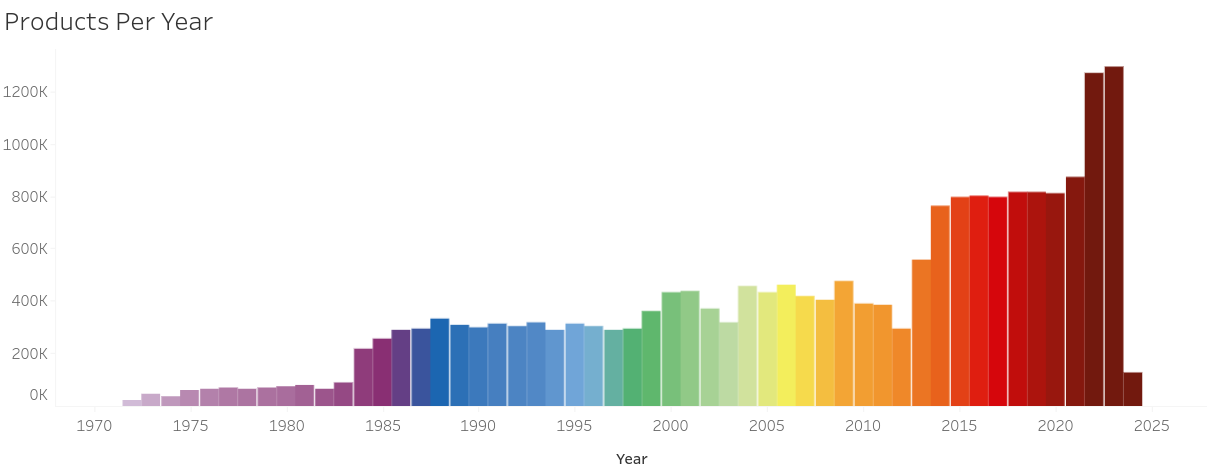
\includegraphics[width=\textwidth]{img/LandsatDataArchiveStatsProductsPerYear.png}
  \caption{Number of Landsat Products per year over time (as of Feb. 2024) by the USGS~\autocite{landsatstats}\label{fig:landsatproductsovertime}}
  \end{figure}
  The rise in availability on the one hand makes it easier for researchers and companies to use the data, but requires increased computing and storage availability, to manage the increased data amount.
  This offers the possibility of creating scientific studies covering a wide range of cities over time, using the same sensor and tools. 
  In~\cite{Sobrino2020} a methodology to compare \glspl{UHI} using \gls{sentinel3} images and conducted a broad study of \glspl{UHI} severity in cities around the world is suggested.
  Over the past years the number of scientific papers investigating the issue from multiple angles increased significantly (ct.~\cite[P. 3]{Piracha2022b}).\\
  In conclusion, the advancement of remote sensing technology, particularly the availability of infrared imagers and satellite imagery, has revolutionized the study of \gls{UHI}. 
  From the early investigations and roots of the field in meteorology and public health the research field expanded touching urban development, climate science, atmospheric chemistry and medicine as well as social sciences.
  The scope of studies from case studies conducted in the 70s to the current abundance of data provided by satellites like Landsat 8 and 9, researchers now have the tools to analyse urban surface temperature distribution with unprecedented detail and accuracy.
  The increase in data availability has not only facilitated research on urban meteorology and heat islands but has also presented new challenges in terms of data management and analysis.
  Despite these challenges, the potential for conducting comprehensive studies across various cities using consistent sensor data and combining multiple sensor sources allows a deep understanding and continuous monitoring of the urban environment.
  %As demonstrated by studies such as the one conducted by \autocite{Sobrino2020} using Sentinel-3 images, the future of \gls{UHI} research holds promise for gaining deeper insights into the impacts of urbanization on local climate patterns worldwide.
  % TODO more and finish
  The next step in advancing the comprehension of \glspl{UHI} involves gaining a deeper understanding of how various parameters contribute to the formation and intensity of \glspl{UHI}.
  With the widespread introduction of countermeasures to \glspl{UHI} and climate change resilience techniques in different cities, continuous monitoring of statistical parameters and indices becomes more relevant in order to assess the effectiveness of the mitigation strategies. 

 \subsection{Research Question}
  In this thesis, the impacts of land cover changes, such as urbanisation, and rising average temperatures on the \gls{UHI} phenomena are investigated.
  The specific questions posed are:
  \begin{enumerate}
    \item What definition can be used to define \glspl{UHI} comparably?\label{q1}
    \item What is the influence of \gls{LULC} change on the size of urban heat islands?\label{q2}
    \item How significant is the impact of urbanisation on \glspl{UHI}, both in terms of absolute and relative temperature changes?\label{q3}
    \item What is the effect of rising average temperatures on the \glspl{UHI} effect?\label{q4}
    \item Is it feasible to model \glspl{UHI} using the identified impacts of temperature and land use change?\label{q5}
    \item What indices can be used or created to categorize and rate \gls{UHI} intensity?\label{q6}
  \end{enumerate}
  The first question tackles the problem that \gls{UHI} definitions changed over time and there are different types of \glspl{UHI} that can be measured. The goal is to find a definition that describes \glspl{UHI} in a comparable way, to allow global measurement and comparison between cities and regions.\\ 
  The second and third question investigates the impact urbanisation and surface sealing on the intensity and size of urban heat islands. This can help in urban planning and mitigation of \glspl{UHI} in affected urban areas.\\ %TODO this sentence 
  The fourth questions goal is to answer how much the rise of global temperatures due to climate change is affecting the intensity of \gls{UHI} effect in cities.% 
  The fifth question aims to provide a methodology and quantify if the \gls{UHI} effect can be modelled and predict the intensity when surface or air temperatures are given. 
  The sixth and last question shall answer what indices that are already given can be used to describe heat islands or if there is the need to create a new index for measuring intensity and human impact of \gls{UHI} effects within cities.

 \subsection{Methodology}\label{sec:methodology}
  To address the outlined research questions, multispectral satellite images are used to extract temperature and surface information. 
  This data is used and processed and urban areas are extracted. 
  The data is compared with measurements from ground based stations and statistical analysis is conducted to answer the questions posed above.

  \subsubsection{Data Sources}\label{ssec:datasources} 
    Multi-spectral visible and thermal infrared satellite images are used to measure and identify \glspl{SUHI} and analyse land surface temperature.
    The used satellite data product is described in \cref{sec:landsat}.
    The \gls{LULC} data is referenced against a \gls{LULC} product for validation.\\ 
    For air temperature data the data of weather stations within the area of interest are used, more details can be found in the \cref{sec:landcoverAnalysis} and \cref{sec:tempanalysis}. 

    \subsubsection{Procedure}\label{ssec:procedure} 
    The satellite data (s.~\cref{sec:landsat}) is selected using filters and manual selection to find cloud free images of the area of interest in the time period that was selected for analysis. 
    The dataset is downloaded and the area of interest is extracted and saved to reduce the data footprint.
    This data set is also used to classify the land cover to allow short term land cover analysis using machine learning algorithms for classification.
    For the further analysis a time series of \gls{LULC} is created for selected cities. 
    From the dataset a longitudinal analysis of \glspl{UHI} intensity over time is created.
    For the select days where satellite cover is available, temperature data and other sources are used to create indices to measure heat stress and other parameters for assessing \glspl{UHI} intensity at the different days.
    This data can then be used to create projections of \glspl{UHI} development based on the findings from \gls{SUHI} measurements and \gls{LULC} analysis.
  \subsection{Structure of the Thesis}\label{ssec:structure} 
    In the introduction as well as \cref{sec:background}, previous work and an overview of the current understanding of the \gls{UHI} effect and research in this area is given. 
    %comparable definition
    \Cref{sec:definition} explains the used adaptation of the proposed methodology by~\cite{Sobrino2020} to create a definition of \glspl{SUHI} that is usable for comparing \glspl{UHI} in different cities.  
    \Cref{sec:LULC} explains how the measurements  and investigations of the impact of \gls{LULC} changes by build up where done.
    In \Cref{sec:UHITempImp} the impact of changing temperatures an increase of extreme weather phenomena on the intensity and seasonal variety of \glspl{UHI} was investigated. 
    After these the \cref{sec:conclusion} combines the findings of the previous chapters, shows what other investigations should be investigated further and where the research could be improved. 
%
\newpage
\section{Background}\label{sec:background}
  \subsection{Urban Heat Islands}
    \glspl{UHI} are areas with increased temperature in urban areas
    Due to increase in global temperature as well as increased occurrence of extreme weather and longer periods of heat waves, this phenomenon will likely increase in intensity and will also occur in cities at higher latitudes (\cite{Sachindra2016},~\cite[p.~904]{Wilby2008}).
    \glspl{UHI} are a spacial phenomenon that occurs on different scales and intensities, this makes observation using remote sensing data a good and widely used approach~\autocite{Weng2003}.\\
    \glspl{UHI} are distinguished into surface and atmospheric \glspl{UHI} as discussed in the sections below. 
    Since the phenomenon is known for a long time, mitigation strategies have been proposed to reduce the impact on well-being and intensity of the \glspl{UHI}.
%
    \subsubsection{Atmospheric Urban Heat Islands}\label{sec:at_uhi}
      Atmospheric \glspl{UHI} is the increased air temperature within an urban area. 
      This are more dependent on weather and local topology and are in part caused by the slower cooling rate of build up land causing responsible for \glspl{SUHI}.
      %Under certain conditions the increased temperature will form a hot air pocket, that will trap the head and reduce airflow from and to the area. \\
      The main factors in forming \glspl{UHI} is the thermal storage capacity of materials used in urban areas like concrete, asphalt and steel, that have a high heat capacity and heat up quickly during the day and emit the stored thermal energy as sensible heat with a delay (eg.~during the night~\autocite{Ramamurthy2014}).
      High surface sealing and lack of vegetation reduce surface water availability and diminish evaporation and the cooling effect of latent heat causing more thermal energy to be available as sensible heat. %todo source (sailor?  or first source)
      Another factor is the heat produced by human activity such as industrial processes and combustion engines.
      As a consequence of higher temperatures, active cooling devices (such as air conditioners) are more frequently used for buildings and vehicles. 
      The emitted thermal energy of these heat pumps further increases the surrounding temperature, reinforcing the effect.
      \\
      There are multiple adverse effects and possible mitigation techniques for the reduction of atmospheric \glspl{UHI} (e.g.~\cite{Nichol1994} and~\cite{Stewart2011}). % list studies.  . 
      %The city climate has been studied extensively since the 1870s
      Advective cooling can be observed when the temperature gradient generated airflow from the cooler surrounding areas towards the hot areas within the city, cooling it down~\autocite{HaegerEugensson1999}. \\
      Urban areas with no close water body (generating sea breezes as well as latent heat transport) and with lower average wind speed are more likely to be affected by urban heat islands~\autocite{Ramamurthy2017}. 
      Higher temperatures due to \glspl{UHI} cause stress to animals and humans increasing health risk due to heat stroke and increased surface level ozone concentration~(see~\cite{Santamouris2020}).%
    \subsubsection{Surface Urban Heat Islands}\label{sec:suhi}
       \glspl{SUHI} are areas of higher surface temperatures within urban areas compared to rural areas due to the materials used and heat from mobility, electrical appliances, heating and cooling as well as less vegetation and higher sealed surfaces that reduce surface water availability~\autocite[pp. 7--12]{EPA2008}. 
       The \glspl{SUHI} are a small scale phenomenon that has a high seasonal variability and is most intense in summer.
       Since atmospheric \glspl{UHI} can not be directly observed using remote sensing data, the terms \gls{UHI} and \glspl{SUHI} are used interchangeably in this document. 
  %
    \newpage
    \subsubsection{Air pollution and Urban Heat Islands}
       \begin{wrapfigure}{r}{0.5\textwidth}
         \begin{center}
         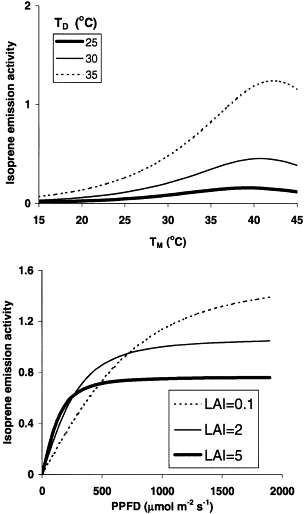
\includegraphics[width=0.48\textwidth]{img/VOCsGraphs}
       \end{center}
       \caption{Temperature dependence of isoprene emission of 15 minute ($T_M$) and 15 day ($T_D$) mean temperature, with permission from~\cite{Guenther2000}}\label{fig:tempVOC}
      \end{wrapfigure}
      Air pollution has been a documented problem for the quality of life since the start of the industrialisation. 
      While in the 19th and first halve of the 20th century the major problem came from unfiltered exhaust of the burning of coal and wood for heating and heavy industry.
      The major pollutants in urban areas in the 21st come from car exhaust and by-products of industrial Agricultural. %TODO sources 
      Especially large urbanized areas are susceptible to air pollution due to increased concentration of combustion and industrial activity on a small area \autocite{Kanakidou2011}.
      One major pollutant with a significant health impact is tropospheric ozone, that is produced in larger quantities within environments with elevated temperature (see~\cite{Ebi2008}). 
      Ozone in the troposphere is mainly produced when (anthropogenic) NO\textsubscript{x} emissions from fossil fuel burning and \glspl{VOC} from anthropogenic or natural sources react with oxygen under UV influence in a photochemical reaction.  
      The creation of ozone is dependent on UV intensity (and therefore insolation) and temperature, increasing between 2.2 and 3.2 ppbv/°C depending on NO\textsubscript{x} and \glspl{VOC} availability. \\
      Recent studies found that reducing NO\textsubscript{x} and \glspl{VOC} reduces O\textsubscript{3} temperature dependence (\cite{Otero2021}).
      Sources of \glspl{VOC} are mainly of natural origin~\autocite{Kansal2009}, anthropogenic sources are vapours and fumes from solvents and mainly originate from industrial processes while the main natural source of \glsps{VOC} are Trees.
      Trees and other plants release VOCs like isoprene and terpenes as a protective mechanism against temperature stress and to protect from insects and pests. 
      The use of these \glspl{VOC} for trees varies over the year and this gives the \gls{VOC} and the resulting O\textsubscript{3} emission a high seasonal variability. 
      The resulting tropospheric ozone, that is major health concern that is directly toxic to humans and is shown to cause lung damage by oxidative stress in the lung lining tissue (see~\cite{Mudway2000}). 
      With rising global temperatures the number of days with temperatures causing heat stress in trees (e.g.\ with a temperature above 30 °C shown in \cref{fig:tempVOC}) has been increasing even at higher altitudes (for the city area of Bremen this ~\cref{fig:ubaTemp}).
      Due to the effect of Urban heat islands that causes a further increase in temperature within urban areas, there is an expected increase of tropospheric ozone due to higher \glspl{VOC} emission from urban and sub urban trees and higher reaction rates in densely populated areas with higher mortality and other health consequences (shown in~\cite{Ebi2008}).\\ 

      \begin{figure}[!htbp]
        \begin{center}
          \includesvg[width=\textwidth]{img/hotdaysbremen}
          \caption{Number of cold and hot days over time in Bremen, Germany\label{fig:ubaTemp}}
        \end{center}
      \end{figure}
      %
    \subsubsection{Mitigation techniques for Urban Heat Islands}\label{ssec:mitigation}
      The attempt to reduce urban heat build-up and the associated heat related health problems in cities is older then scientific work on this field of study. 
      In hot areas around the globe different methods where used to create spaces with cooler temperatures for rest and work. 
      All over the Mediterranean houses are painted white to increase reflection of sunlight. 
      In newer studies this traditional painting pattern has shown to be an efficient counter to high solar intensities \autocite{Fayad2021}.
      % Many cultures use passive cooling  roofs TODO find paper also passive ventilation and such 
      Another method of larger scale cooling is the increase of vegetation to increase latent heat transport and water availability.
      Green roof concepts, green facades, parks or street trees all show effective in reducing temperatures within the urban environment (see~\cite{Ramamurthy2014, Feyisa2014, Dimoudi2003, Gartland2008}).
      Adding water bodies inside the city as well as ``sponge-city''-concepts are also promising approaches to mitigate heat islands (\cite{He2019}).
    \subsubsection{Used Satellites}\label{sec:landsat}
      \begin{figure}[htbp]
       \begin{center}
         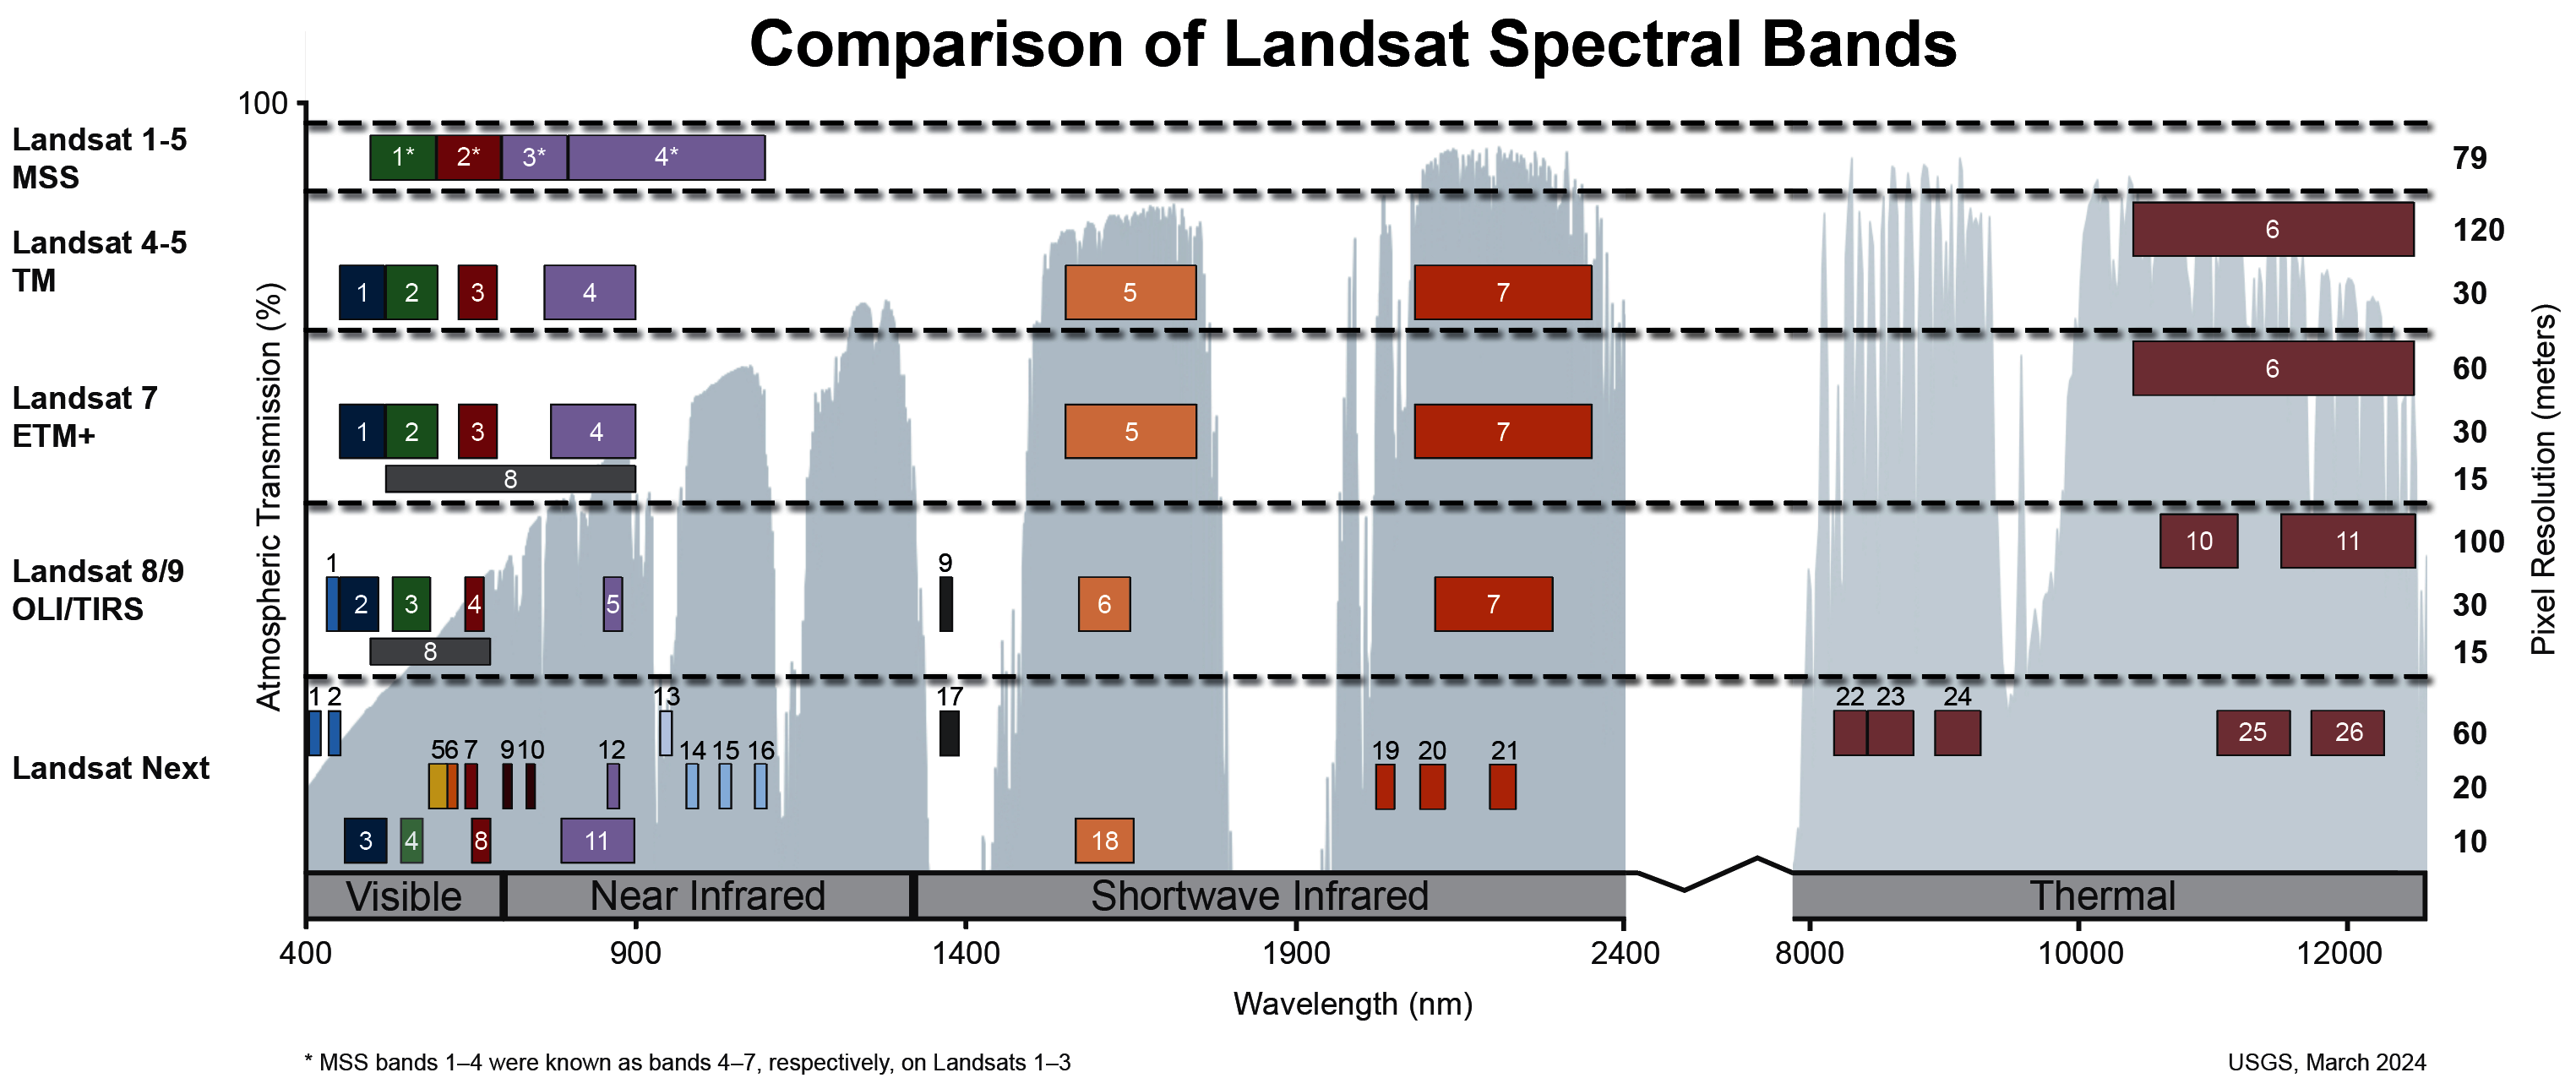
\includegraphics[width=\textwidth]{img/LandsatSpectralBands.png}
       \end{center}
       \caption{Landsat 8 and 9 instrument spectral bands (second to last row) compared to other Landsat missions\autocite{USGSWebsite}\label{fig:lsspectral}}
      \end{figure}
      \noindent
      Using remote sensing data to detect and analyse \gls{SUHI} requires devices that are able to detect thermal infrared radiation. 
      Satellites that are equipped with thermal infrared sensors that are able to detect upwelling emission from the surface temperature within the $ 8\mu m < \lambda < 12\ \mu m $ range. 
      Instruments that were previously used for measuring \glspl{UHI} are Landsat, MODIS, ASTER and Sentinel-3. 
      In the following steps data from the Landsat 8 and Landsat 9 satellites was used.%, as well as Landsat 7 satellites images for historical data from before the launch of Landsat 8. 
      Landsat 8 and Landsat 9 both have a TIRS (Thermal Infrared Sensor) and an OLI (Operational Lands Imager) instrument on board that measure in two and 9 bands respectively.
      Since the start of Landsat 9 the availability of scenes increased and the shorter revisit times allow a denser mapping and reduced risk of cloud cover. \\ 
      The OLI covers a wavelength of 0.43 $\mu m$ to 1.83 $\mu m$ separated into 9 bands with a resolution of 30 m per Pixel (see \cref{fig:lsspectral}). 
      For the calculation of thermal infrared emission of the Earth's surface the TIRS instrument contains two bands within the thermal infrared covering wavelength between 10.6 $\mu m$ and 12.51 $\mu m$ with a resolution of 100 m.
      Both satellites have a revisit time of roughly 14 days. 
  %
  \subsection{Land Surface Temperature}\label{ssec:lst}
    Land surface temperature is the temperature at which an object emits infrared radiation according to plank's law~\autocite{Liang2020}.
    Using remote sensing methods this quantity can not be directly observed since the satellite is observing \gls{TOA} brightness temperature.
    This temperature can be transformed to a \gls{LST} using atmospheric correction and correction for the emissivity of the ground.
    The conversion factor is data source dependent and can be found in \cref{sec:lstcalc}.
%
  \subsection{Air Temperature}\label{ssec:airtemperature}
    Urban heat islands that directly impact human health are the atmospheric \glspl{UHI} in the urban canopy layer. 
    These are defined by the air temperature from street level up to roof height. 
    The air temperature within the urban area is warmed differently from the air temperature outside the urban area, due to higher thermal mass that buildings and sealed surfaces have and less latent heat transport.
    %
    During the day the air temperature is lower then the surface temperature~\autocite{EPA2008}, during the night the hot surfaces radiate off the energy heating the surrounding air.\\
    %
    There are multiple additional factors impacting urban air temperature. 
    Combustion from traffic and industrial processes produce heat as a by-product that heats the surrounding air. 
    HVAC systems also produce heat, when cooling buildings. 
    This further increases the air temperature increasing cooling need within the urban area, creating a positive feedback loop. 
    \newpage
    \subsection{Indices}
Many different indices are used for analysis of images or parameters in remote sensing, atmospheric physics and meteorology.
The following sections introduce the indices that where used to analyse the \glspl{UHI} within this work. 
\subsubsection{NDVI}
\textit{The following section is a slightly reworked version of a section from the pre-thesis master project~\cite{andrae2023}}\\ 
%
\noindent
\begin{figure}[!htbp]
    \centering
    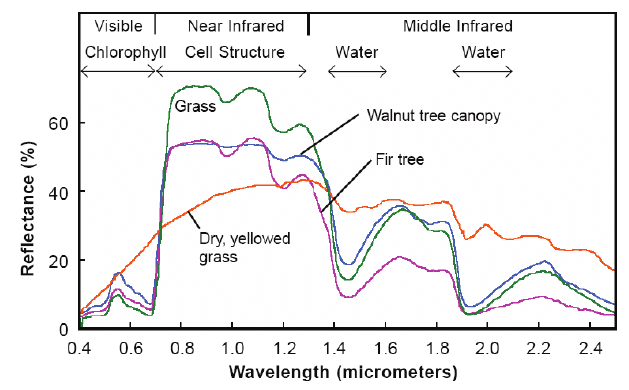
\includegraphics[width=0.5\textwidth]{img/Reflectance-spectra-of-different-types-of-green-vegetation-compared-to-a-spectral.png}
    \caption{Absorption spectrum of green vegetation \autocite[P. 5]{Smith2012}\label{fig:absorbtionVeg}}
\end{figure}
The \gls{NDVI} is an widely used index using the difference of the red and near infrared bands to determine the amount of green vegetation. 
\begin{equation}
    NDVI = \frac{Red-NIR}{Red+NIR}
    \label{equ:ndvi}
\end{equation}
For Landsat 8 and 9 data, channel 4 (red $640\ \text{nm} - 670\ \text{nm}$) and channel 5 (near infrared $850\ \text{nm} - 880\ \text{nm}$) where used.
As shown in \cref{fig:absorbtionVeg} healthy plants reflect near infrared and there is a sharp rise in reflectance between the two used channels at around $700\ \text{nm}$. 
%
This index is used for emissivity estimation for Land Surface Temperature calculation see \cref{equ:toa}, correlation with heat islands (since there is a negative correlation between those two values, due to the latent heat of evaporation reducing surface temperature at higher vegetation areas).
\begin{figure}[!htbp]
    \centering
    \begin{subfigure}{0.45\textwidth}
    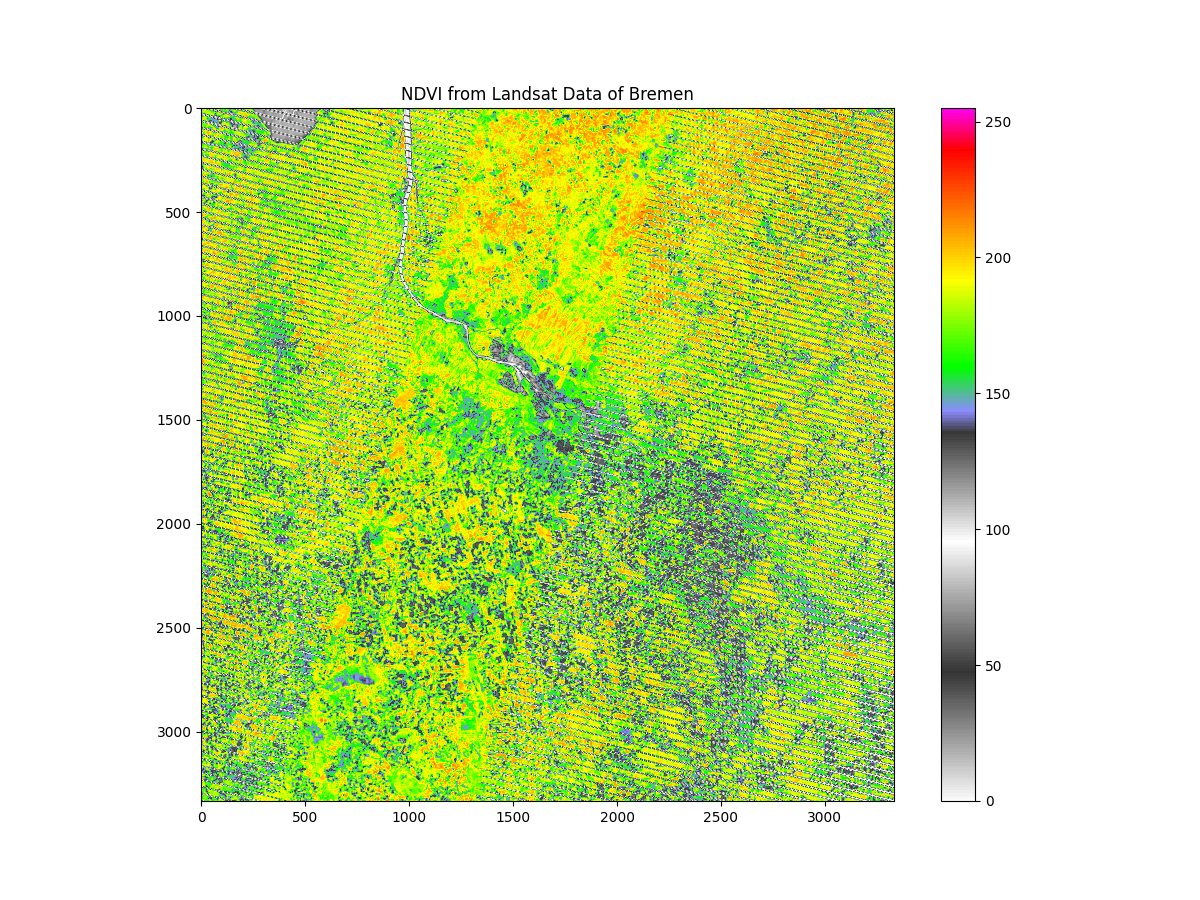
\includegraphics[width=\textwidth]{img/NDVI_LE07_L1TP_196023_20190723_20200825_02_T1__Bremen.png}
    \subcaption{NDVI of Bremen (Bands 5 and 6) using Landsat 7 data on 2019--07--23}
    \end{subfigure}
    \begin{subfigure}{0.45\textwidth}
    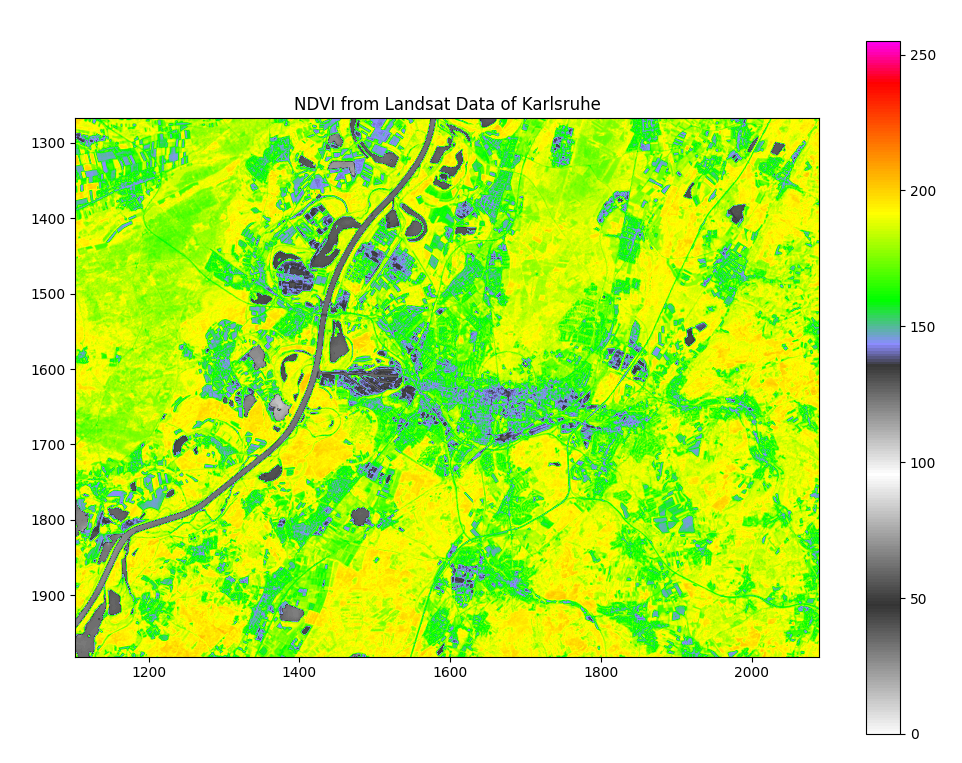
\includegraphics[width=\textwidth]{img/KarlsruheNDVI_Landsat8.png} 
    \subcaption{NDVI of Karlruhe (Bands 4 and 5) using Landsat 8 data on 2023--06--07}
    \end{subfigure}
    \caption{NDVI Images from the different satellites\label{fig:ndvi}}
\end{figure}
%\subsubsection{NDVI Colormap}\label{sec:colormap}
%When using a classical heat map with a color gradient from colder to warmer colors or a diverging color map (see \cref{fig:ndviPhoenixAzBad}), details of the image get lost and it is hard to distinguish plant heath, build up and vegetated areas and the difference between small \gls{NDVI} changes.
%To aid an intuitive understanding a specially created colormap can be used. 
%The color map was adapted for use in python from work of \texttt{public lab}\cite{ndviCmap} where it was developed in an attempt to create color-blind friendly \gls{NDVI} color maps.
%Values below 0.2 are areas with no vegetation.
%The color map used in \cref{fig:ndviPhoenixAz} uses a gradient of gray with a ``black-white-black
%white'' transition to allow higher dynamic range for non vegetation areas.
%For areas with an \gls{NDVI} $<$ 0.2 blue is used. Green values are low or unhealthy green vegetation or mixed use pixels. 
%Orange and red values correspond to thicker vegetation e.g.~forests, parks or green fields. 
%%
%Comparing \cref{fig:ndviPhoenixAz}  and \cref{fig:ndviPhoenixAzBad} where most of the desert surrounding the city has no green vegetation and the parts covered in vegetation can be clearly distinguished from the arid desert regions.
%Still the surface roughness can be seen quite well due to the gray scale gradient in the $<$ 0.2 \gls{NDVI} range.  
%%
%\begin{figure}[htbp]
% \centering
%    \begin{subfigure}{0.46\textwidth}
%    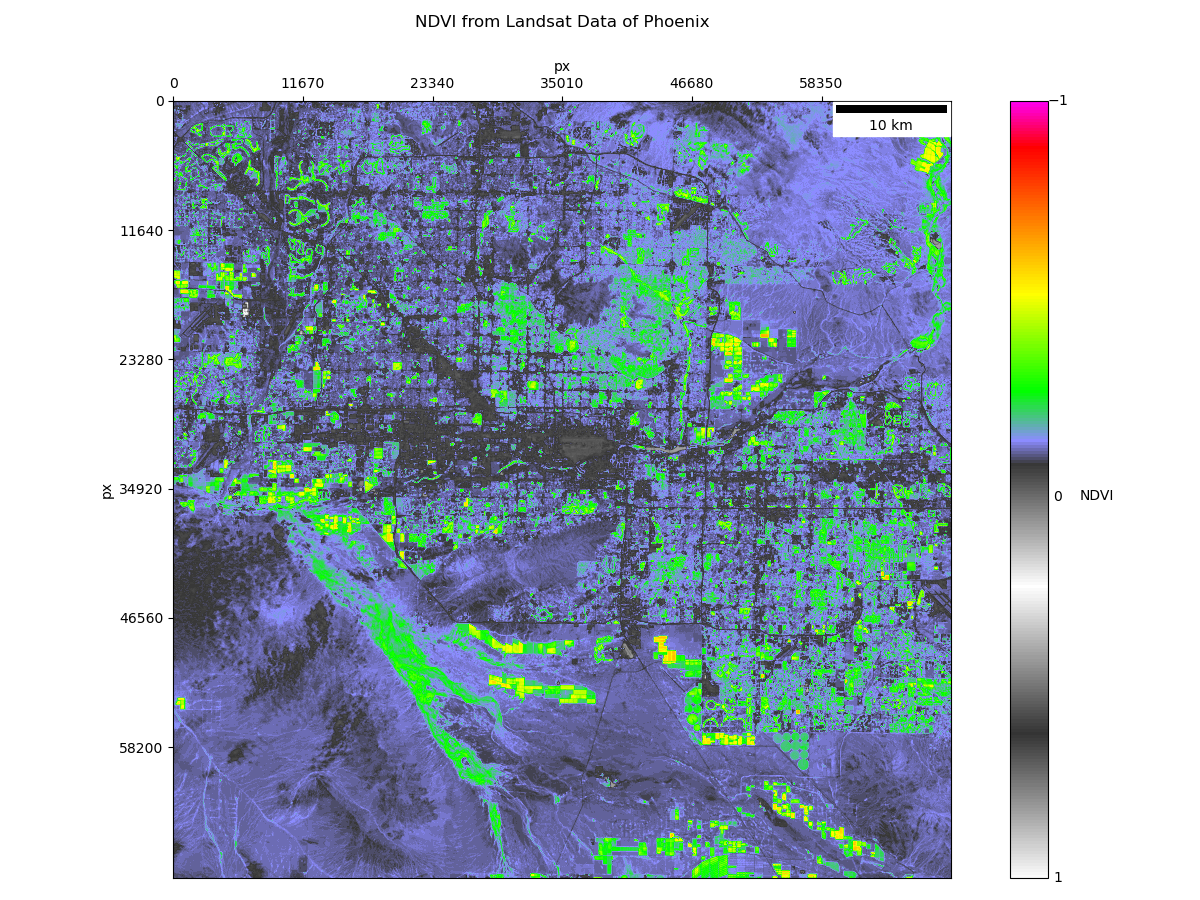
\includegraphics[width=\textwidth]{img/NDVI from Landsat Data of Phoenix.png} 
%    \subcaption{NDVI Image of Phoenix with the  VGYRM color map\label{fig:ndviPhoenixAz}}
%    \end{subfigure}
%    \begin{subfigure}{0.46\textwidth}
%    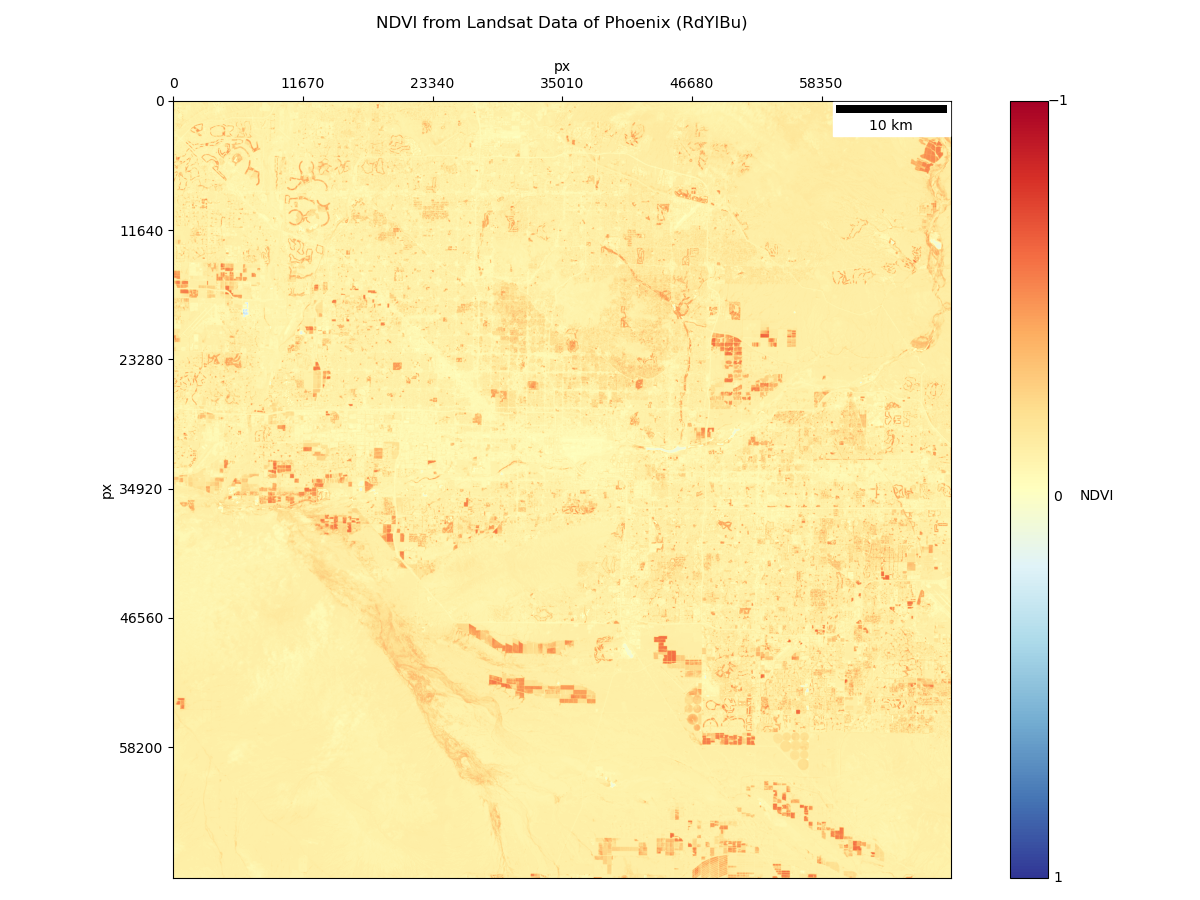
\includegraphics[width=\textwidth]{img/NDVI from Landsat Data of Phoenix (RdYlBu).png} 
%    \subcaption{NDVI Image of Phoenix with a RdYlBu gradient color map\label{fig:ndviPhoenixAzBad}}
%    \end{subfigure}
%    \caption{Different color maps used show the better ability to differentiate between green vegetation and desert and buildings within Phoenix\label{fig:ndvicomp}}
%\end{figure}

    \subsubsection{Heat Index}
    The \gls{HI}is a temperature index that takes sultriness into account and rates the impact of temperature and air humidity of the human body. 
    The output of this temperature scale (given in °C) is the apparent temperature, depending on relative air humidity. 
    The defined range is between 20 °C and 50°C dry bulb temperature and up to 90\% relative humidity~\autocite[p. 862]{Steadman1979}. 
    The proposed heat index is based on a model human and takes wind chill and clothing into account, to produce a apparent temperature of human. 
    The heat index can be used as a good reference for non-extreme conditions. 
    Its biggest downside is the missing account for direct insolation on body temperature and comfort.
    The Heat Index later is used to compare different \glspl{UHI} with each other.
%%
  \subsection{Wet Bulb Globe Temperature}
    To account the impact of insolation on the human body and how it reacts to heat stress differently in different environmental condition s, the Wet Bulb Globe Temperature was developed. 
    Working under heat stress poses a serious health issue, for this the \gls{WBGT} was defined as EN ISO 7243:2017 (\cite{Iso7243_2017}), calculating the thermal load on the human body.
    Heat exchange between the human body and the environment is dominated by evaporation of secreted sweat.
    The efficiency of this process is determined by the vapor pressure, that is influenced by temperature difference and the humidity difference. %TODO ref paper with caves
    The Heat Index is a simple way of calculating this efficiency that does not take radiant heat into account, the WBGT does incorporated this effect in the calculation.
    %#The WTGB is not used on the analysis later, since the insolation in northern europe is significantly low TODO add or rm?
      \newpage
\section{Image Processing}\label{sec:imgProcessing}
    Using remote sensing data for scientific purposes requires a 
    \begin{itemize} 
      \item[a] systematic
      \item[b] reproducible
      \item[c] verifiable 
    \end{itemize}%
    way of detecting patterns and information within the data. \\
    The field of image processing and machine learning has developed a wide range of tools that are used in many different fields over the past decades. % TODO might want to add examples here ?

    \subsection{Machine Learning}\label{sec:ml}
      The term machine learning describes a set of algorithms that use a set of training data, detect statistical correlations using different weights to approximate this data. %TODO external source 
      These approximations can be stored and be used to detect the same features within new but similar data.
      Different machine learning techniques are used for for different use cases and areas.
      %In total 
%
      In the next sections the image processing steps are described from a technical perspective and the underlying mathematical frameworks are discussed.
    \subsection{Data Processing Pipeline}
      An image or data processing pipeline is a chained list of processing steps, that allows to feed different data through the same algorithm. 
      Many different data processing and machine learning \glspl{lib} use these to allow flexibility and modularity of the steps in data processing (e.g.\ the used~\cite{scikit-learn},~\cite{keras} or~\cite{gluon}). 
      The data processing was done using a \textit{scikit-learn} pipeline for data analysis as well as multiple other \glspl{lib}. 
      In \cref{fig:pipeline} the overview of the different steps within the data processing can be seen.
      \begin{figure}[!htbp]
         \begin{subfigure}[b]{0.40\textwidth}
           \begin{tikzpicture}[node distance=2cm, auto, scale=.5, on grid]
  \node (start) [startstop, text width=0.7\textwidth] {Start};
  \node (input) [io, below of=start, text width=0.6\textwidth]{Landsat 8\ \& 9 Image};
  \node (cut) [process, below of=input, text width=0.9\textwidth]{Cut to AOI};
  \node (features) [process, below of=cut, text width=0.9\textwidth]{Gabor Feature Extraction};
  \node (kmeans) [process, below of=features, text width=0.9\textwidth]{KMeans clustering};
  \node (stat1) [process, below of=kmeans, text width=0.9\textwidth]{Statistical analysis of different classes};
  \node (stat2) [process, below of=stat1, text width=0.9\textwidth]{manual class name assignment};
  \node (verif) [process, below of=stat2, text width=0.9\textwidth]{verification of classification};
  \node (diff) [process, below of=verif, text width=0.9\textwidth]{diff analysis of LU/LC classes};
  \node (stop) [startstop, below of=diff,text width=0.7\textwidth] {Stop};

  \draw[arrow] (start) -- (input);
  \draw[arrow] (input) -- (cut);
  \draw[arrow] (cut) -- (features);
  \draw[arrow] (features) -- (kmeans);
  \draw[arrow] (kmeans) -- (stat1);%(randomforest);
  %\draw[arrow] (randomforest) -- (stat1);
  \draw[arrow] (stat1) -- (stat2);
  \draw[arrow] (stat2) -- (verif);
  \draw[arrow] (verif) -- (diff);
  \draw[arrow] (diff) -- (stop);
\end{tikzpicture}

           \subcaption{Processing pipeline for developing the model}\label{fig:pipelineTraining}
         \end{subfigure}
         \begin{subfigure}[b]{0.40\textwidth}
           \begin{tikzpicture}[node distance=2cm, auto, scale=.5, on grid]
  \node (start) [startstop, text width =0.7\textwidth] {Start};
  \node (input) [io, below of=start, text width =0.6\textwidth]{Landsat 7\& 8 Image};
  \node (cut) [process, below of=input, text width = 0.9\textwidth]{Cut to AOI};
  \node (features) [process, below of=cut, text width = 0.9\textwidth]{Gabor Feature Extraction};
  \node (randomforest) [process, below of=features, text width = 0.9\textwidth]{Surface Classification \\using the trained model};
  \node (stat1) [process, below of=randomforest, text width = 0.9\textwidth]{Urban area detection using Random Forrest};
  \node (stat2) [process, below of=stat1, text width = 0.9\textwidth]{Statistical analysis of image areas};
  \node (diff) [process, below of=stat2, text width = 0.9\textwidth]{LU/LC change detection};
  \node (uhi) [process, below of=diff, text width = 0.9\textwidth]{UHI detection};
  \node (timeline) [process, below of=uhi, text width = 0.9\textwidth]{analyse change over time};

  \draw[arrow] (start) -- (input);
  \draw[arrow] (input) -- (cut);
  \draw[arrow] (cut) -- (features);
  \draw[arrow] (features) -- (randomforest);
  \draw[arrow] (randomforest) -- (stat1);
  \draw[arrow] (stat1) -- (stat2);
  \draw[arrow] (stat2) -- (diff);
  \draw[arrow] (diff) -- (uhi);
  \draw[arrow] (uhi) -- (timeline);
\end{tikzpicture}

           \subcaption{Data Processing pipeline with the trained Model}\label{fig:pipelineTrained}
         \end{subfigure}
         \caption{The image processing overview\label{fig:pipeline}}
       \end{figure}
  \newpage
  \subsection{Gabor Feature Detection}\label{sec:gabor}
    The Gabor filter is an linear filter, that uses a convolution of an image with a wavelet created by rotating a sine modulated Gaussian, this kernel type is also called the \textit{gabor wavelet}. 
    In image processing this algorithm is used as an feature extraction algorithm to extract and analyse texture and structures with different sizes within the image~(\autocite{Cerdan1993}). 
    By rotating the kernel and changing the frequency, different textures are extracted from the image.
    %
    Mathematically the Gabor-filter is defined by
    \begin{equation}
      g(x,y; \lambda, \theta, \phi, \sigma, \gamma) = \exp \left(- \frac{x'^2 + \gamma^2\cdot y'^2}{2\sigma^2}\right) \cdot \exp \left[i \left(2\pi\frac{x}{\lambda} + \phi \right)\right] 
    \end{equation}
    With $ x' = x \cos(\phi) + y \sin(\phi)~\text{and}~y' = -x \sin(\phi) + y \cos(\phi)$.
    The x and y parameter determine the kernel size, this parameter should be chosen based on the image size and expected structure length.\\
    $\gamma$ is the aspect ratio of the kernel, with $\gamma = 1$ the kernel is round, for smaller $\gamma$ the kernel becomes a more eccentric ellipse.\\
    $\phi$ is the angle of rotation of the sine component of the kernel. \\
    $\theta$ is the angle of rotation of the kernel, detecting differently oriented features.\\
    $\lambda$ is the wavelength of the sine wave. \\
    $\sigma$ is the standard deviation of the Gaussian distribution\\ \\
    %TODO add more accurate description of parameters
    To detect different structures of different scales within the image, a filter bank can be created by combining multiple filters and varying $\phi$, $\sigma$ and $\theta$.\\
    After the convolution of the image with the filter bank, the resulting set of detected features can be used as an input into different algorithms.
    \Cref{fig:gaborExample} shows different kernel sizes and rotations on an satellite image of Bremen. 
    It can be seen that the different structures such as fields (seen in \cref{fig:feat02} and \cref{fig:feat05}) or larger structures and water bodies (seen in \cref{fig:feat01} and \cref{fig:feat03}).
    The output of the filter is an tensor that contains a binary image sized matrix per filter. Each layer provides meta information for each pixel, if it is part of a larger scale texture or pattern. 
    This meta information is used to add additional features for the surface classification (\cref{sec:classification}) using K-Means %(in training) and 
    to allow better classification.%using the random forest model.
    \begin{figure}[!htbp]
       \centering
     \begin{subfigure}[b]{0.45\textwidth}
         \centering
         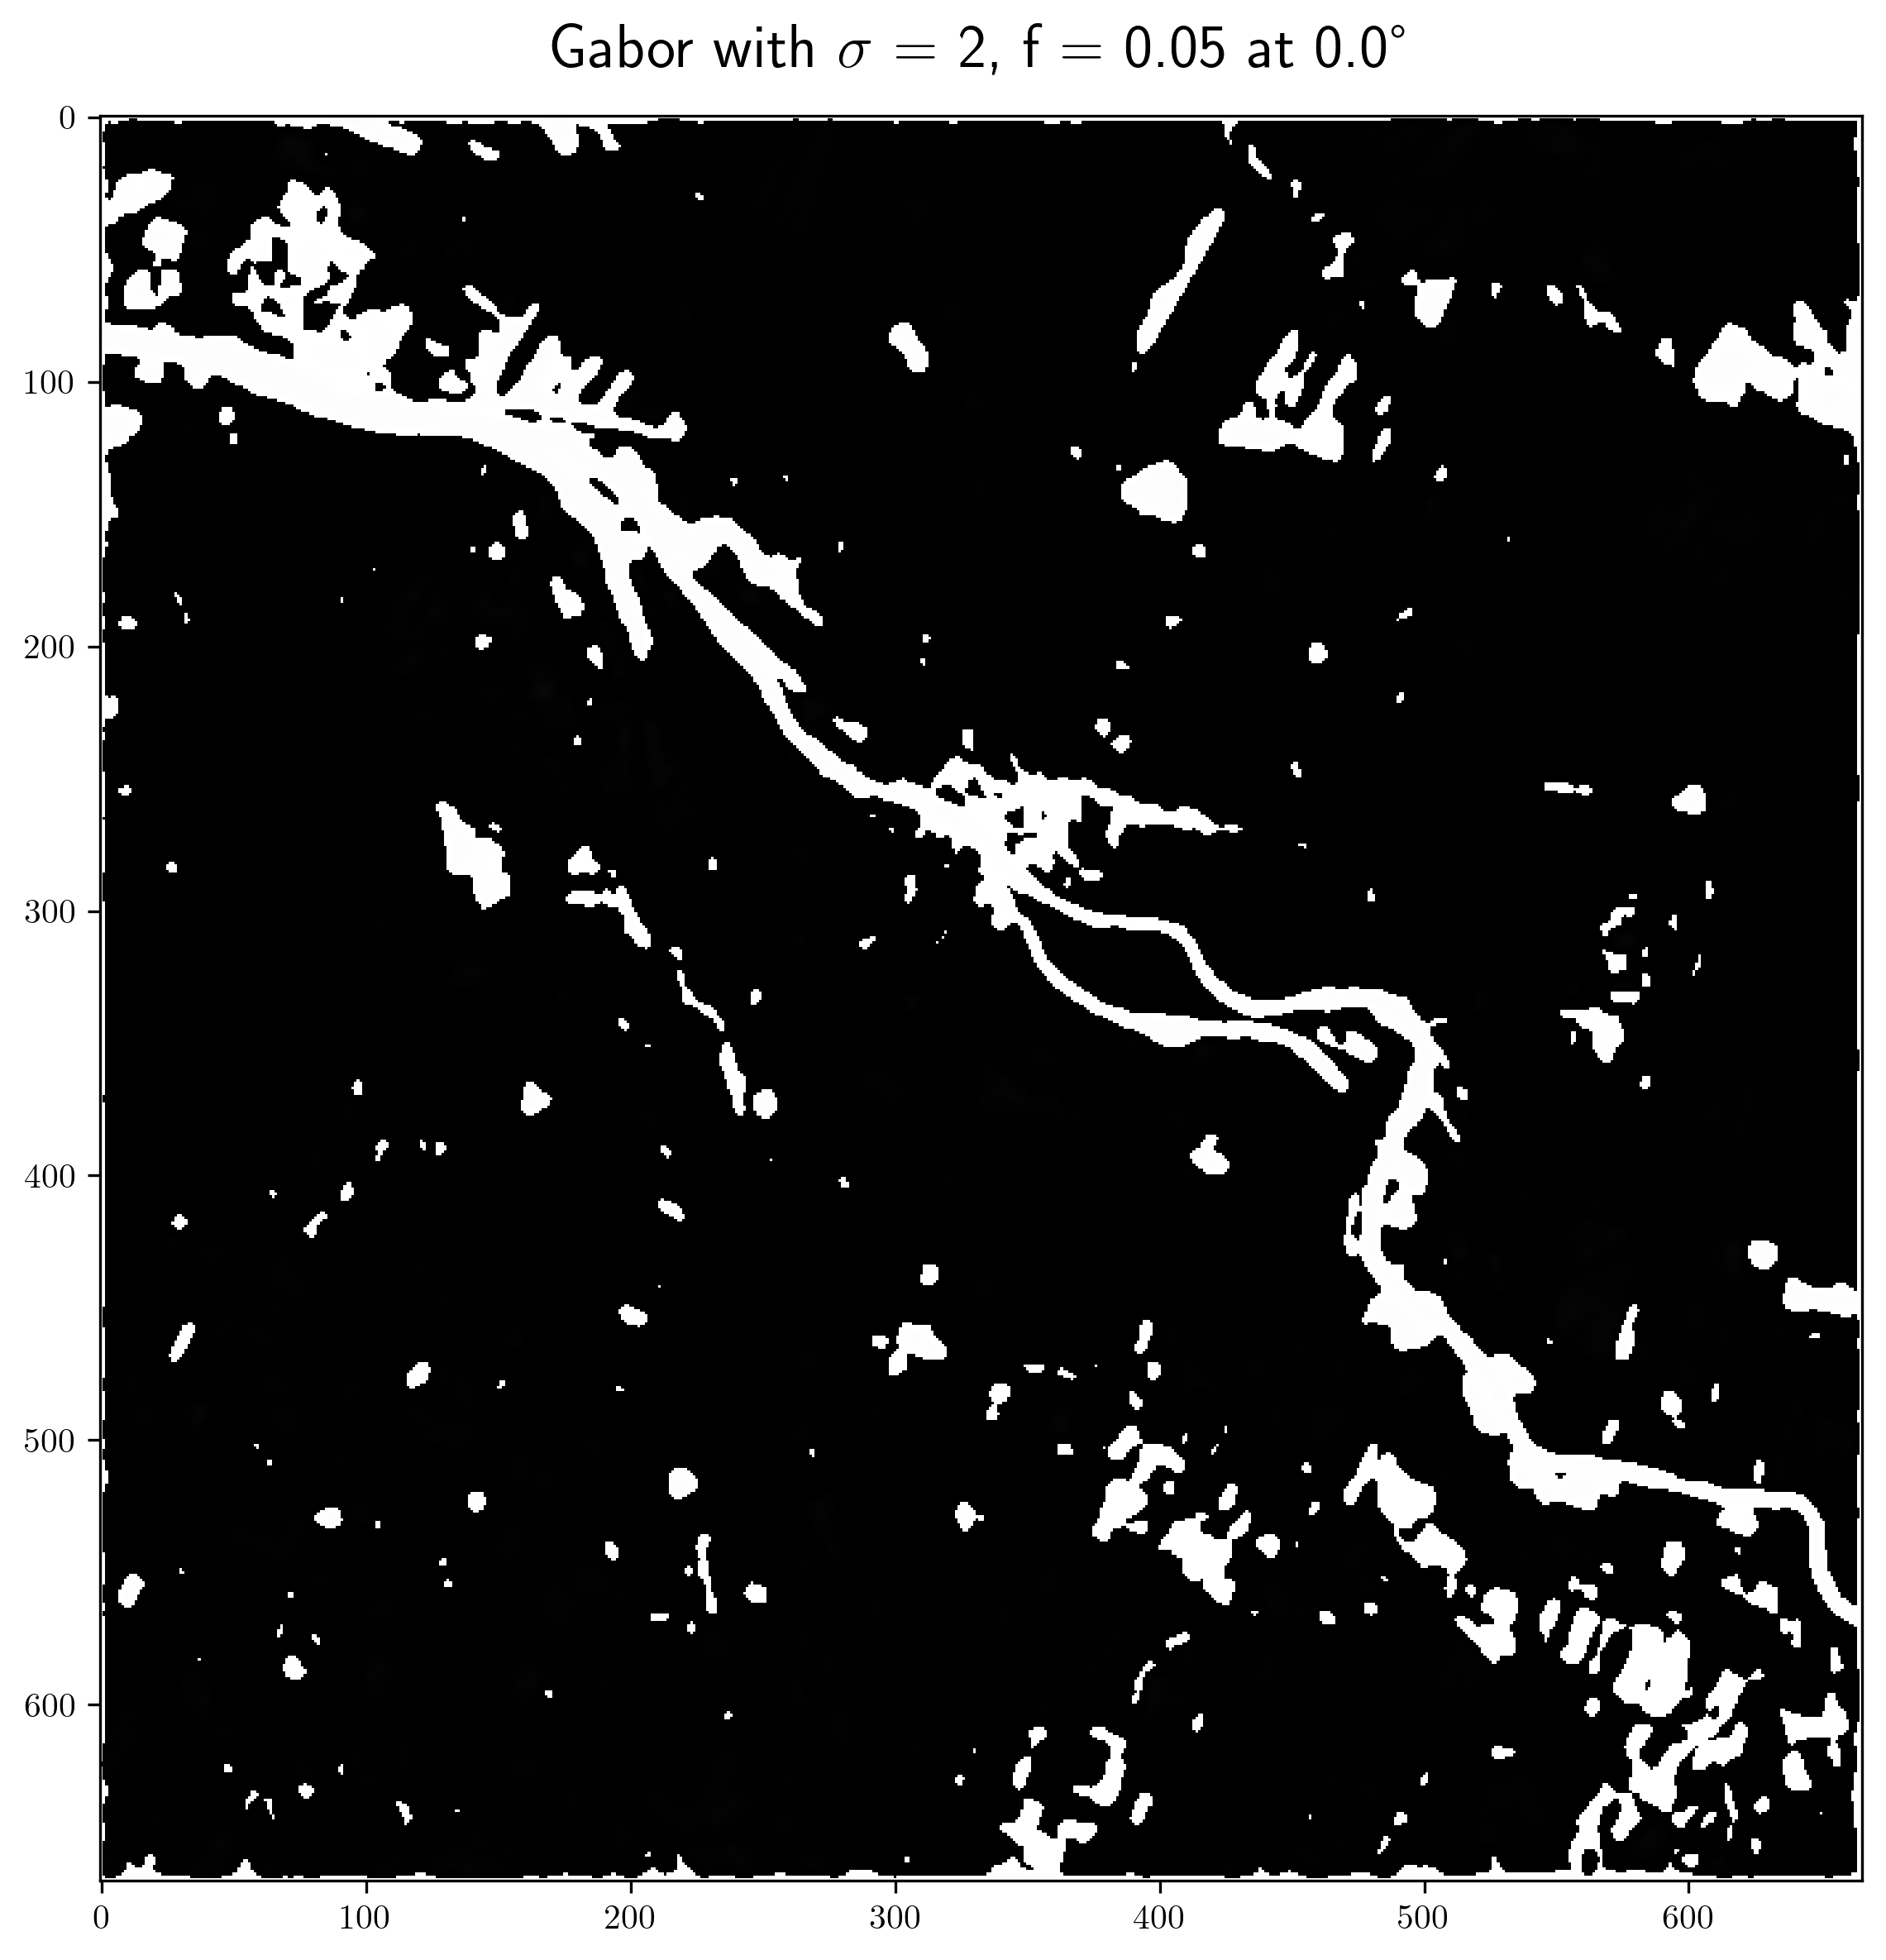
\includegraphics[width=\textwidth]{img/Features_2_005_0.png}
         \subcaption{Kernel with $\sigma$ = 2, f = 0.05 and 0 ° rotation}\label{fig:feat01}
     \end{subfigure}
     \hfill
     \begin{subfigure}[b]{0.45\textwidth}
         \centering
         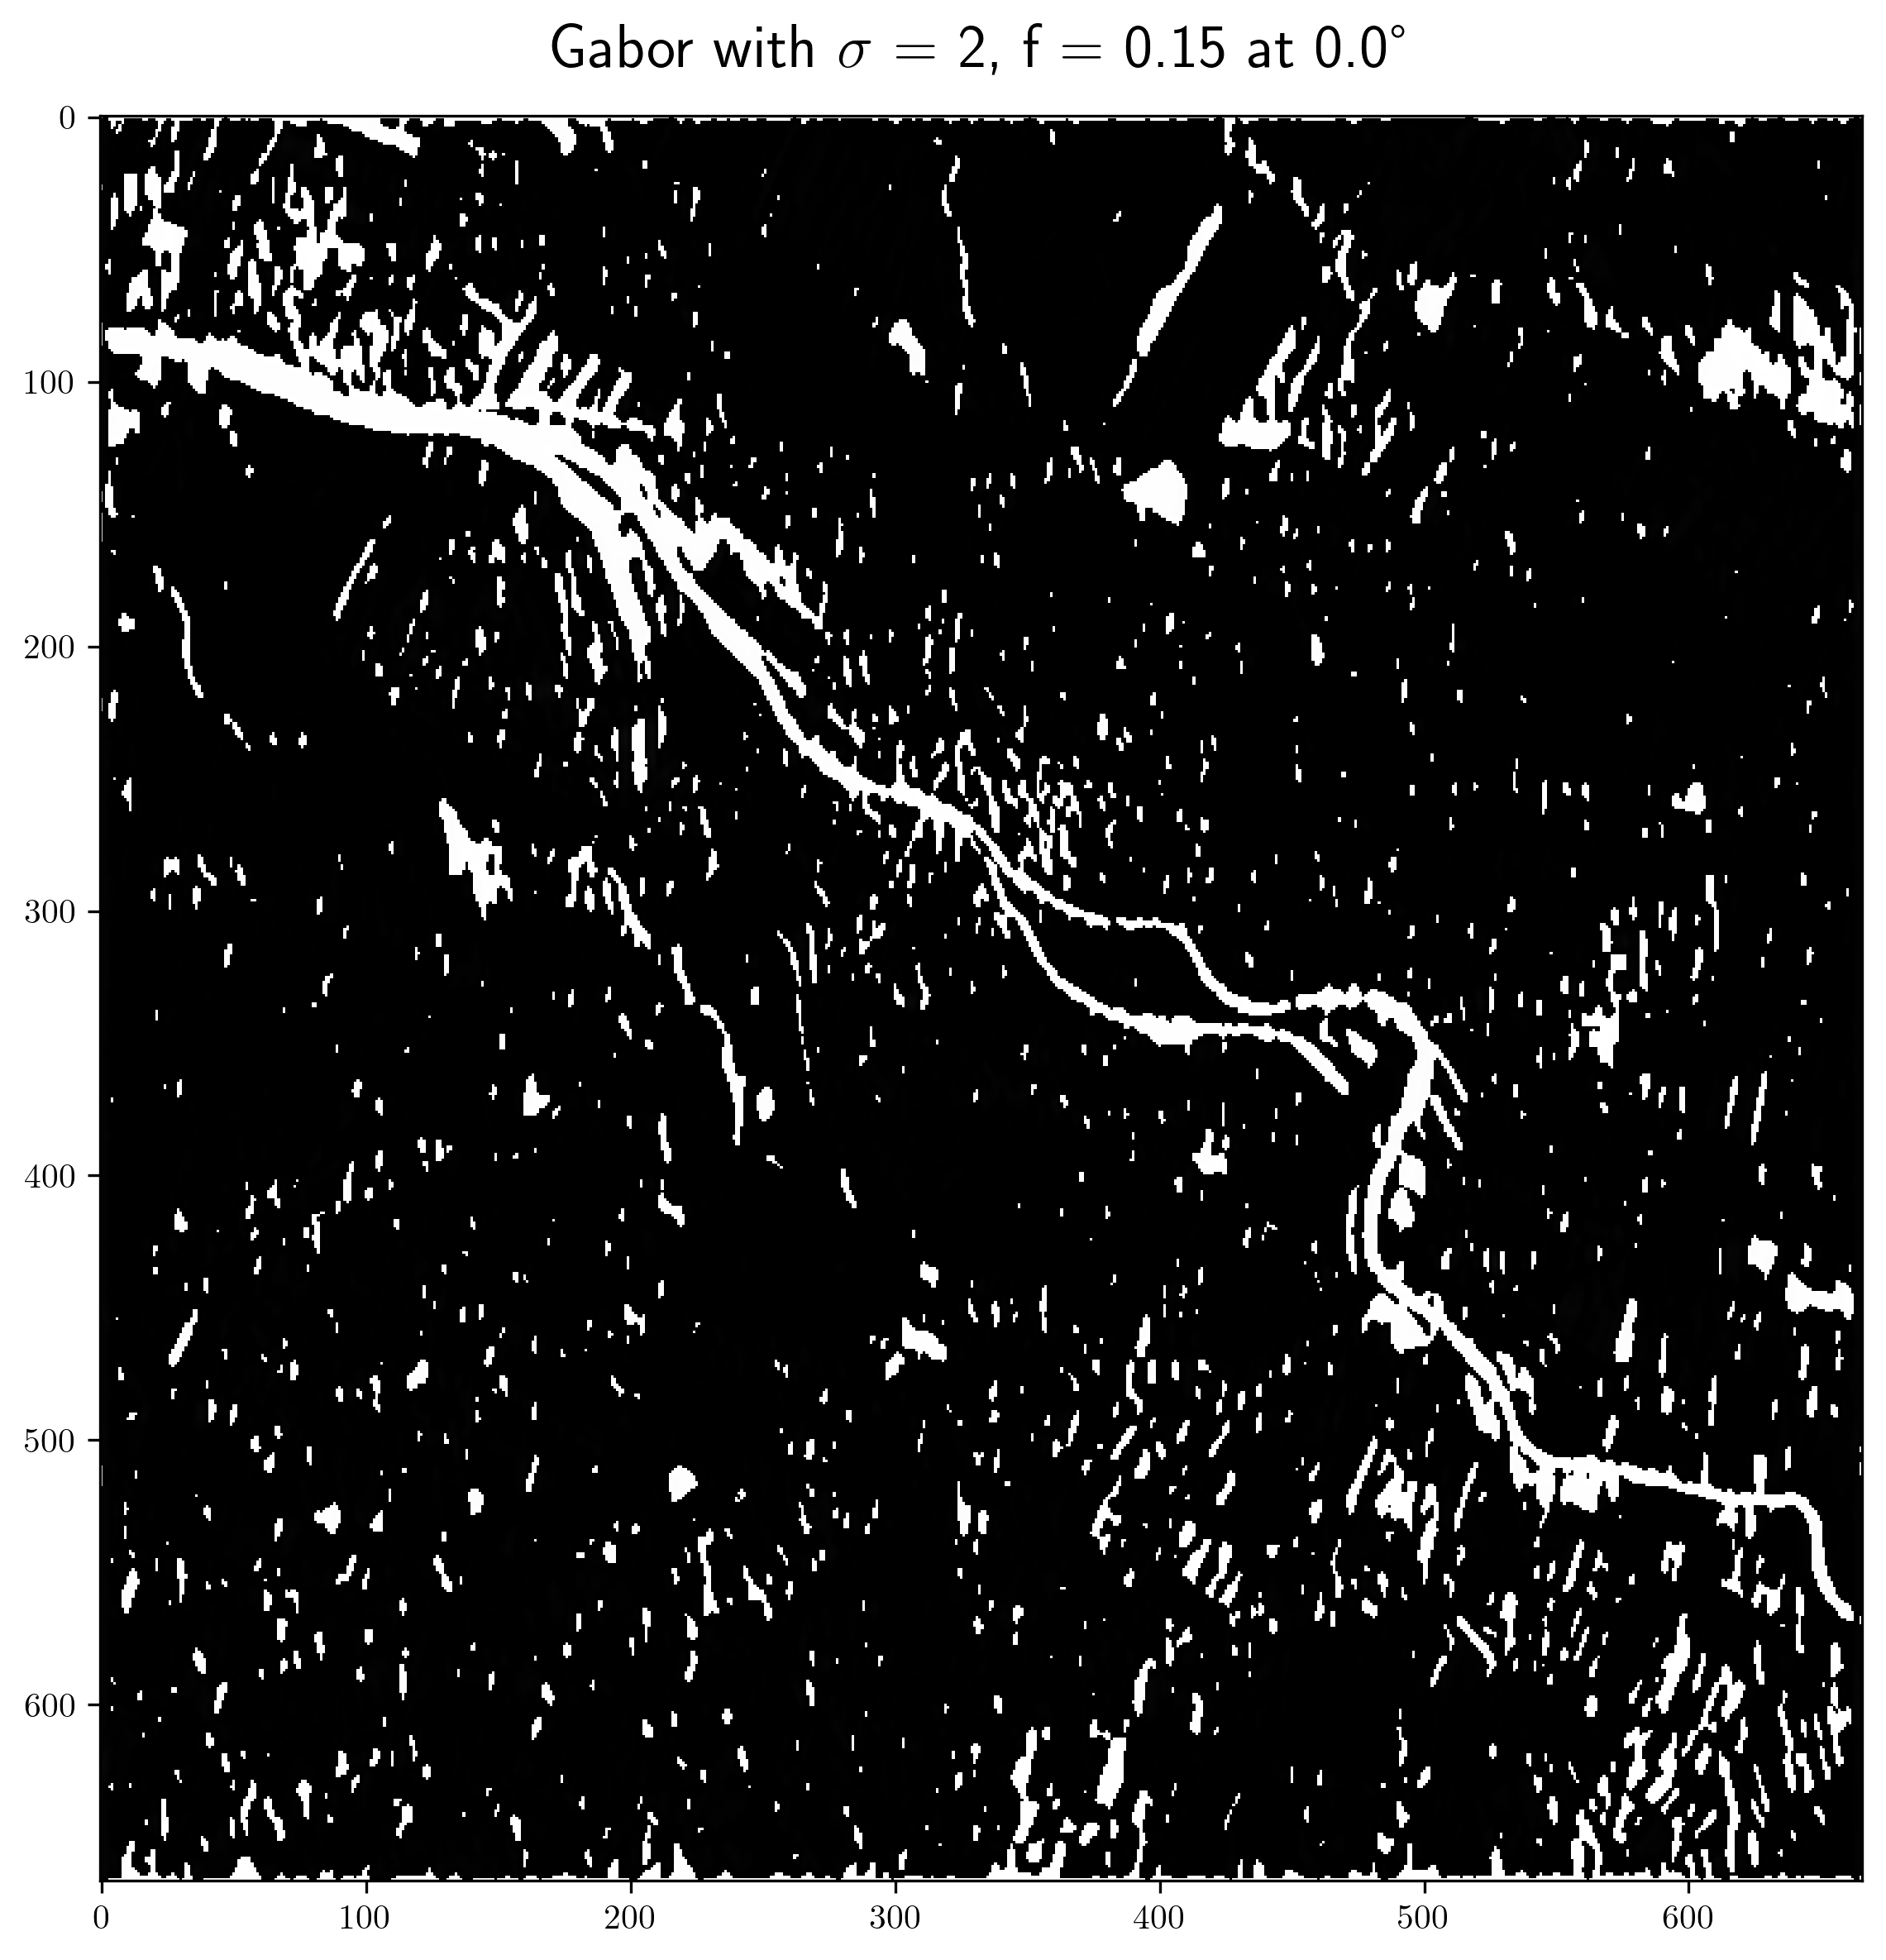
\includegraphics[width=\textwidth]{img/Features_2_015_0.png}
         \subcaption{Kernel with $\sigma$ = 2, f = 0.15 and 0 ° rotation}\label{fig:feat02}
     \end{subfigure}

     \begin{subfigure}[b]{0.45\textwidth}
         \centering
         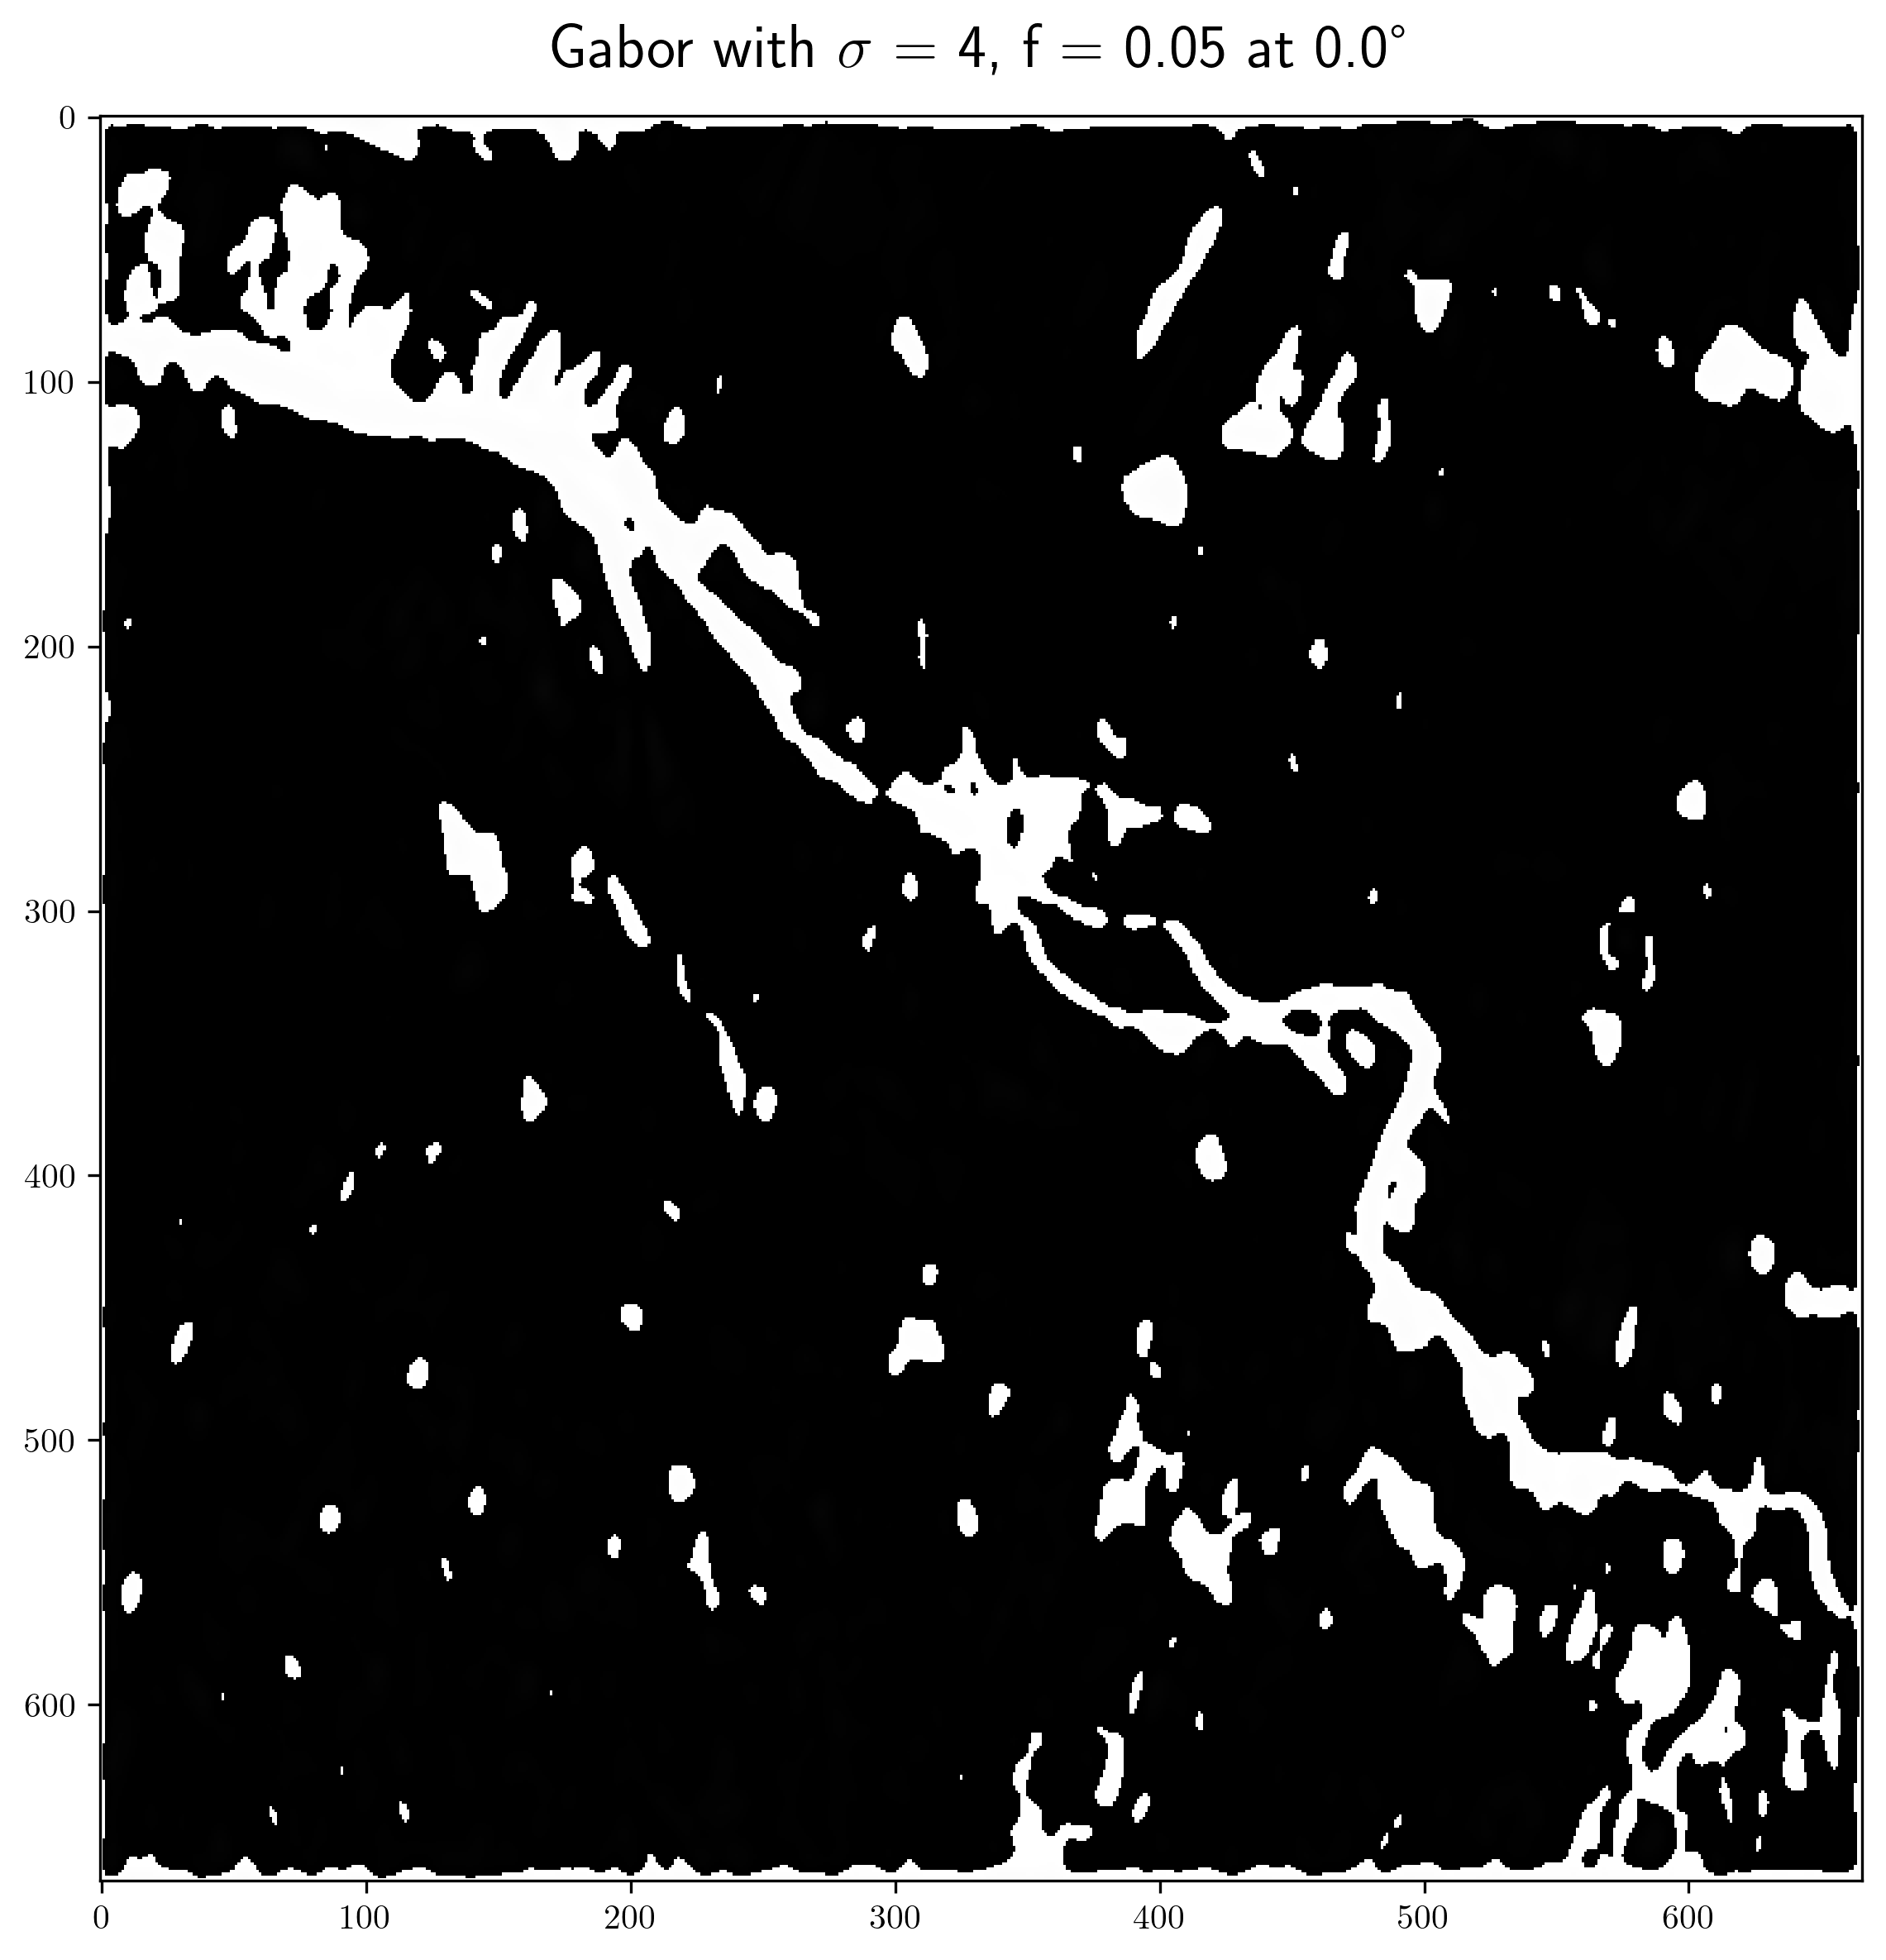
\includegraphics[width=\textwidth]{img/Features_4_005_0.png}
         \subcaption{Kernel with $\sigma$ = 4, f = 0.05 and 0 ° rotation}\label{fig:feat03}
     \end{subfigure}
     \hfill
     \begin{subfigure}[b]{0.45\textwidth}
         \centering
         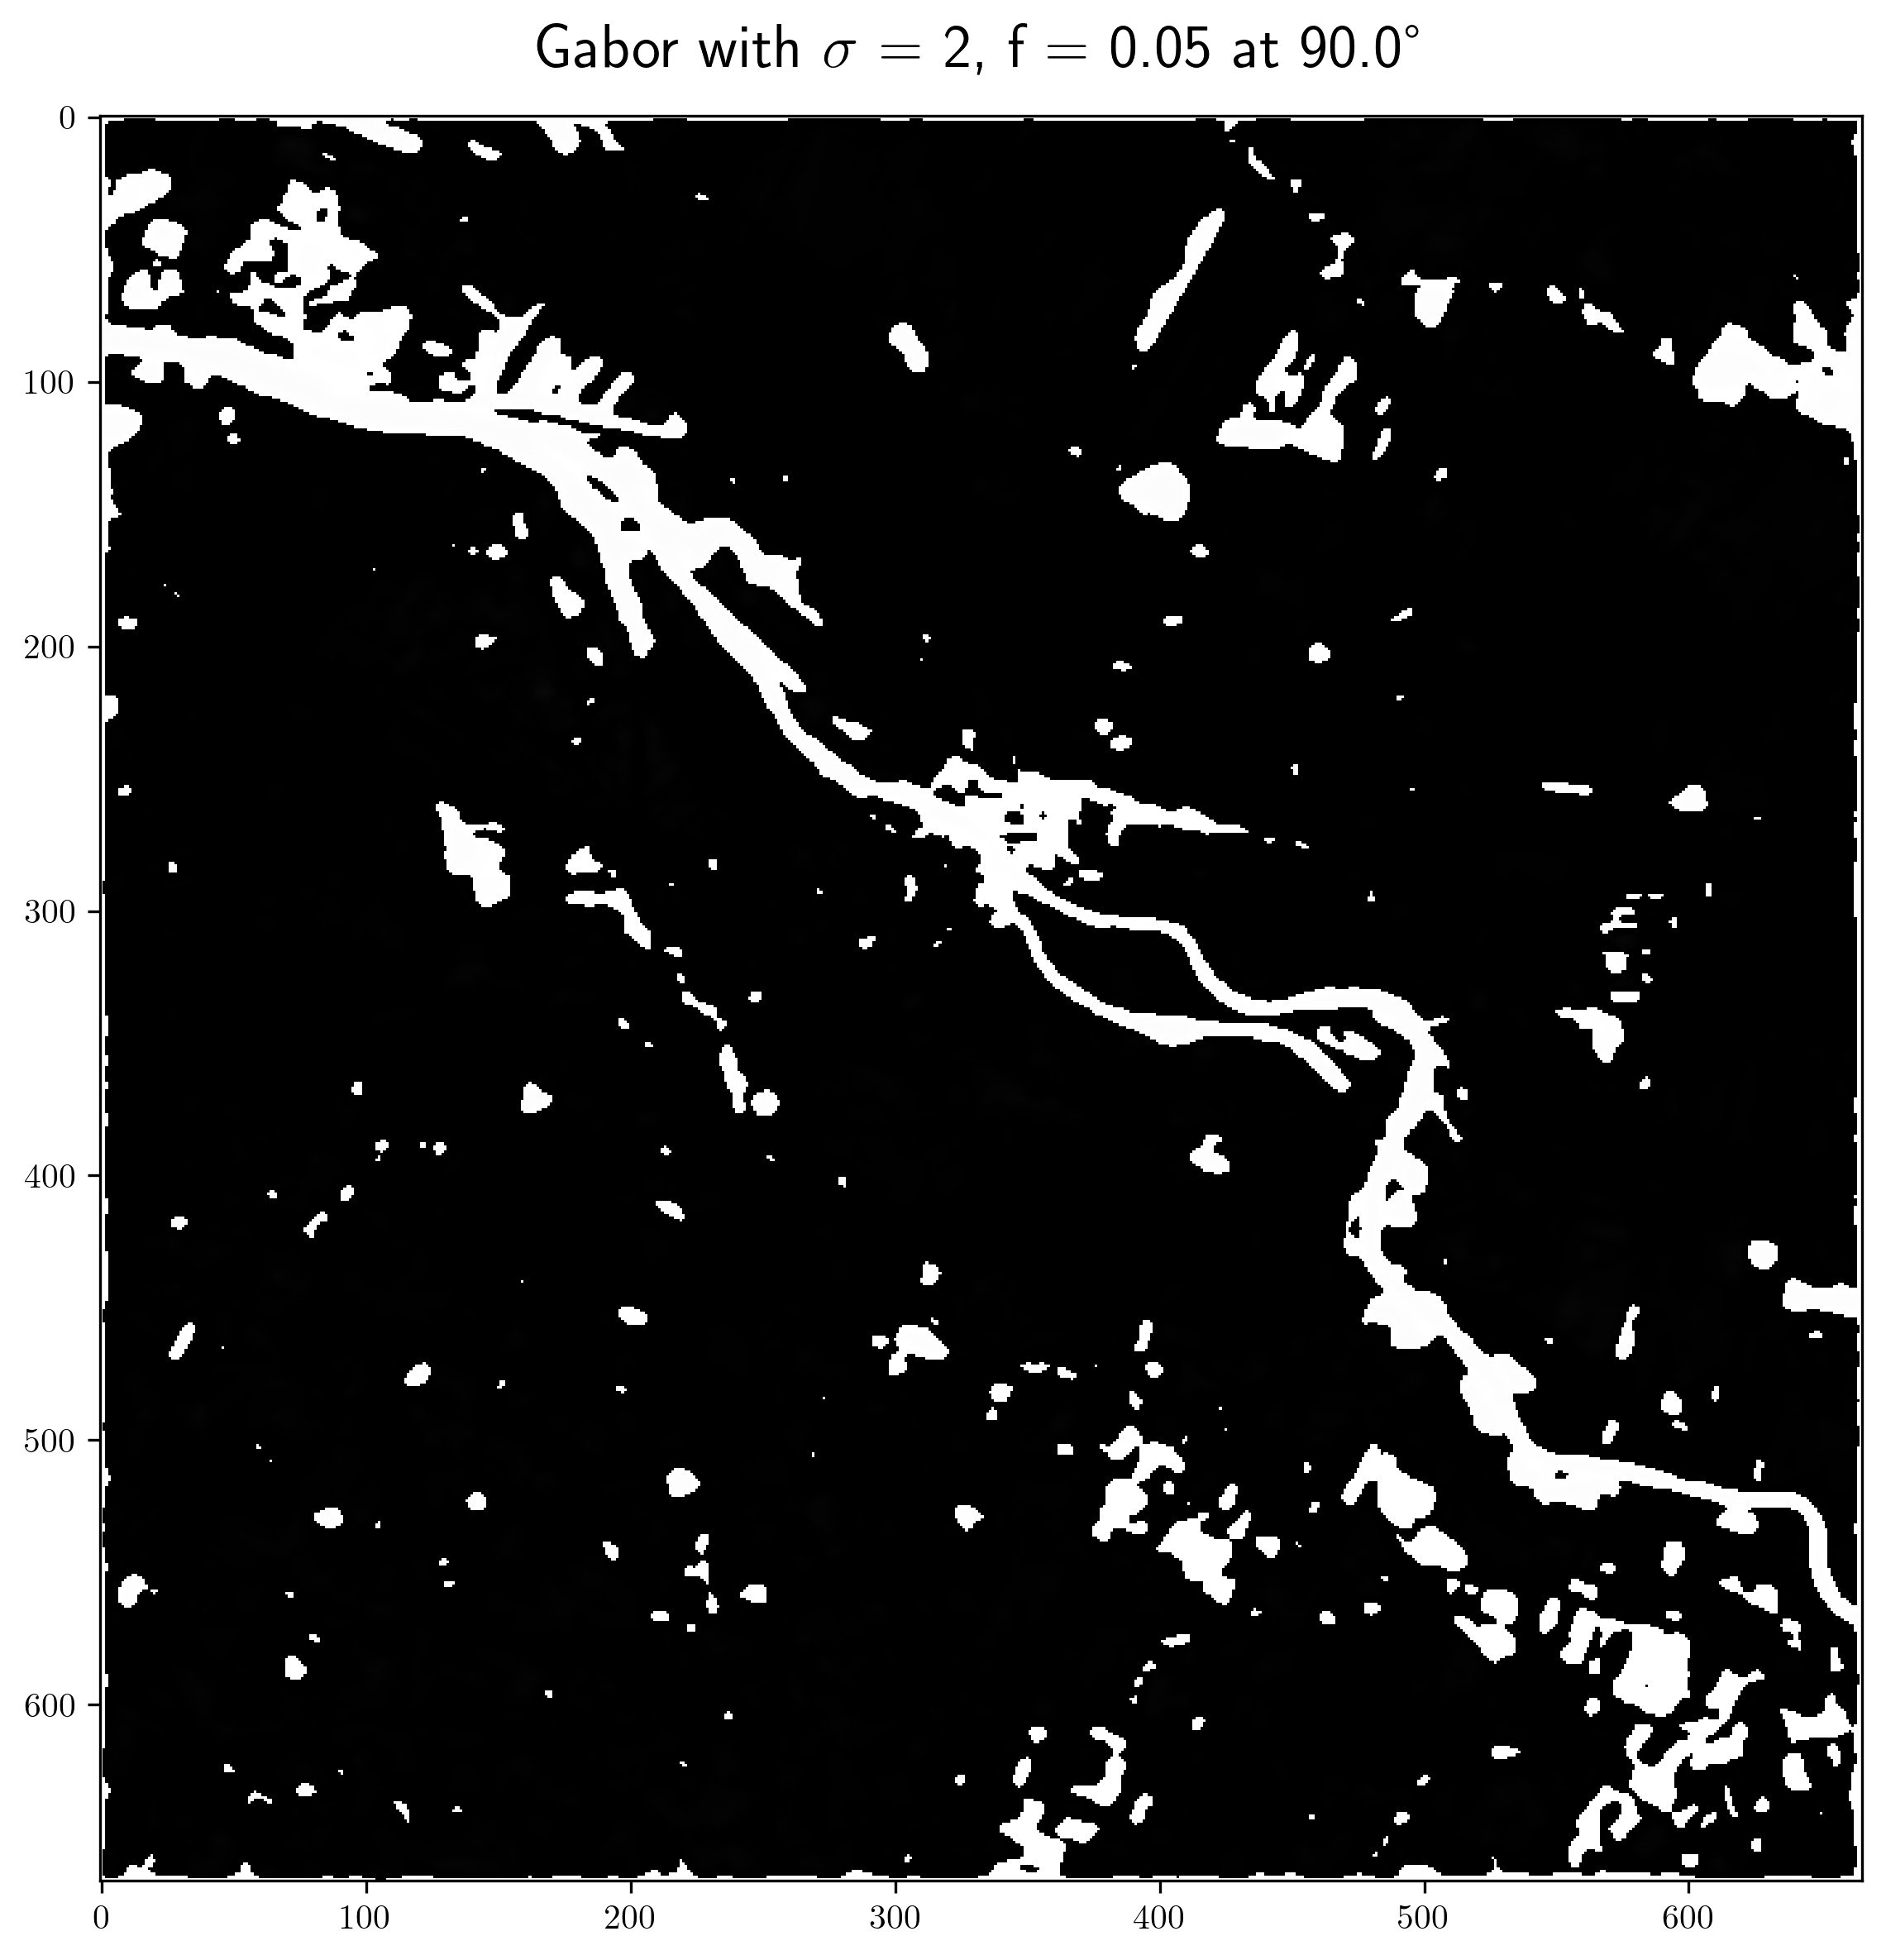
\includegraphics[width=\textwidth]{img/Features_2_005_90.png}
         \subcaption{Kernel with $\sigma$ = 2, f = 0.05 and 90 ° rotation}\label{fig:feat04}
     \end{subfigure}

     \begin{subfigure}[b]{0.45\textwidth}
         \centering
         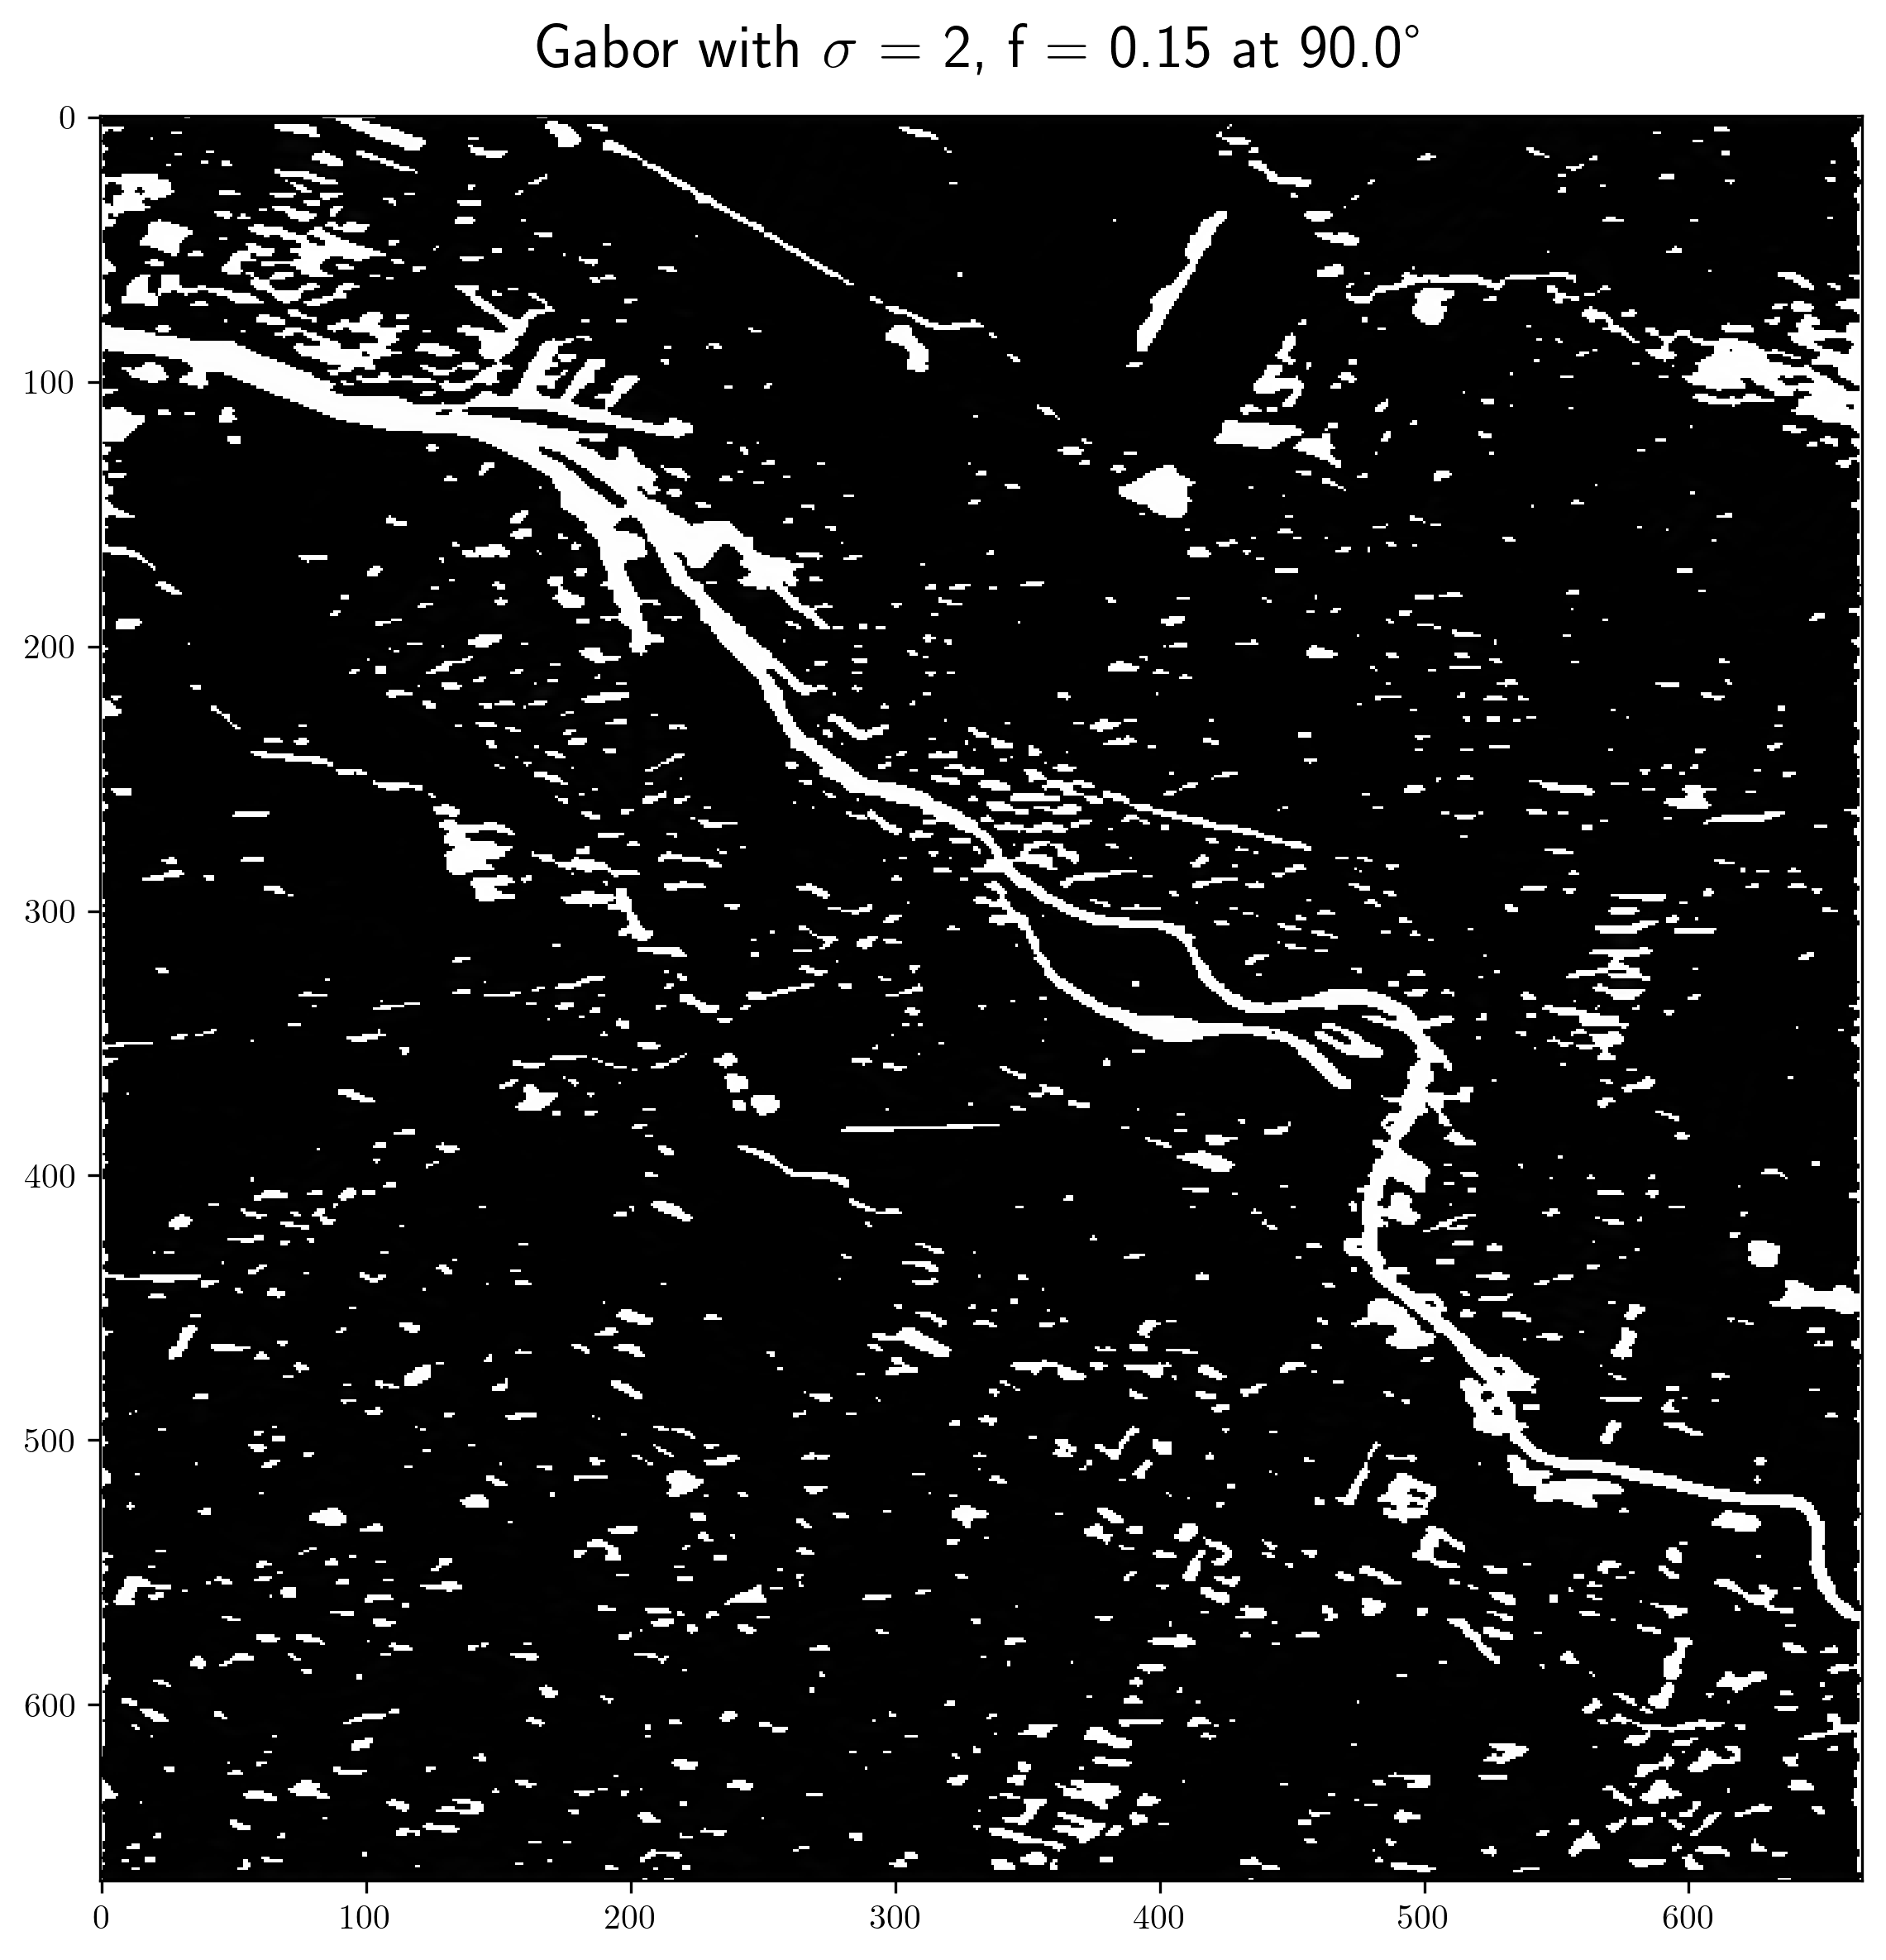
\includegraphics[width=\textwidth]{img/Features_2_015_90.png}
         \subcaption{Kernel with $\sigma$ = 2, f = 0.15 and 90 ° rotation}\label{fig:feat05}
     \end{subfigure}
     \hfill
     \begin{subfigure}[b]{0.45\textwidth}
         \centering
         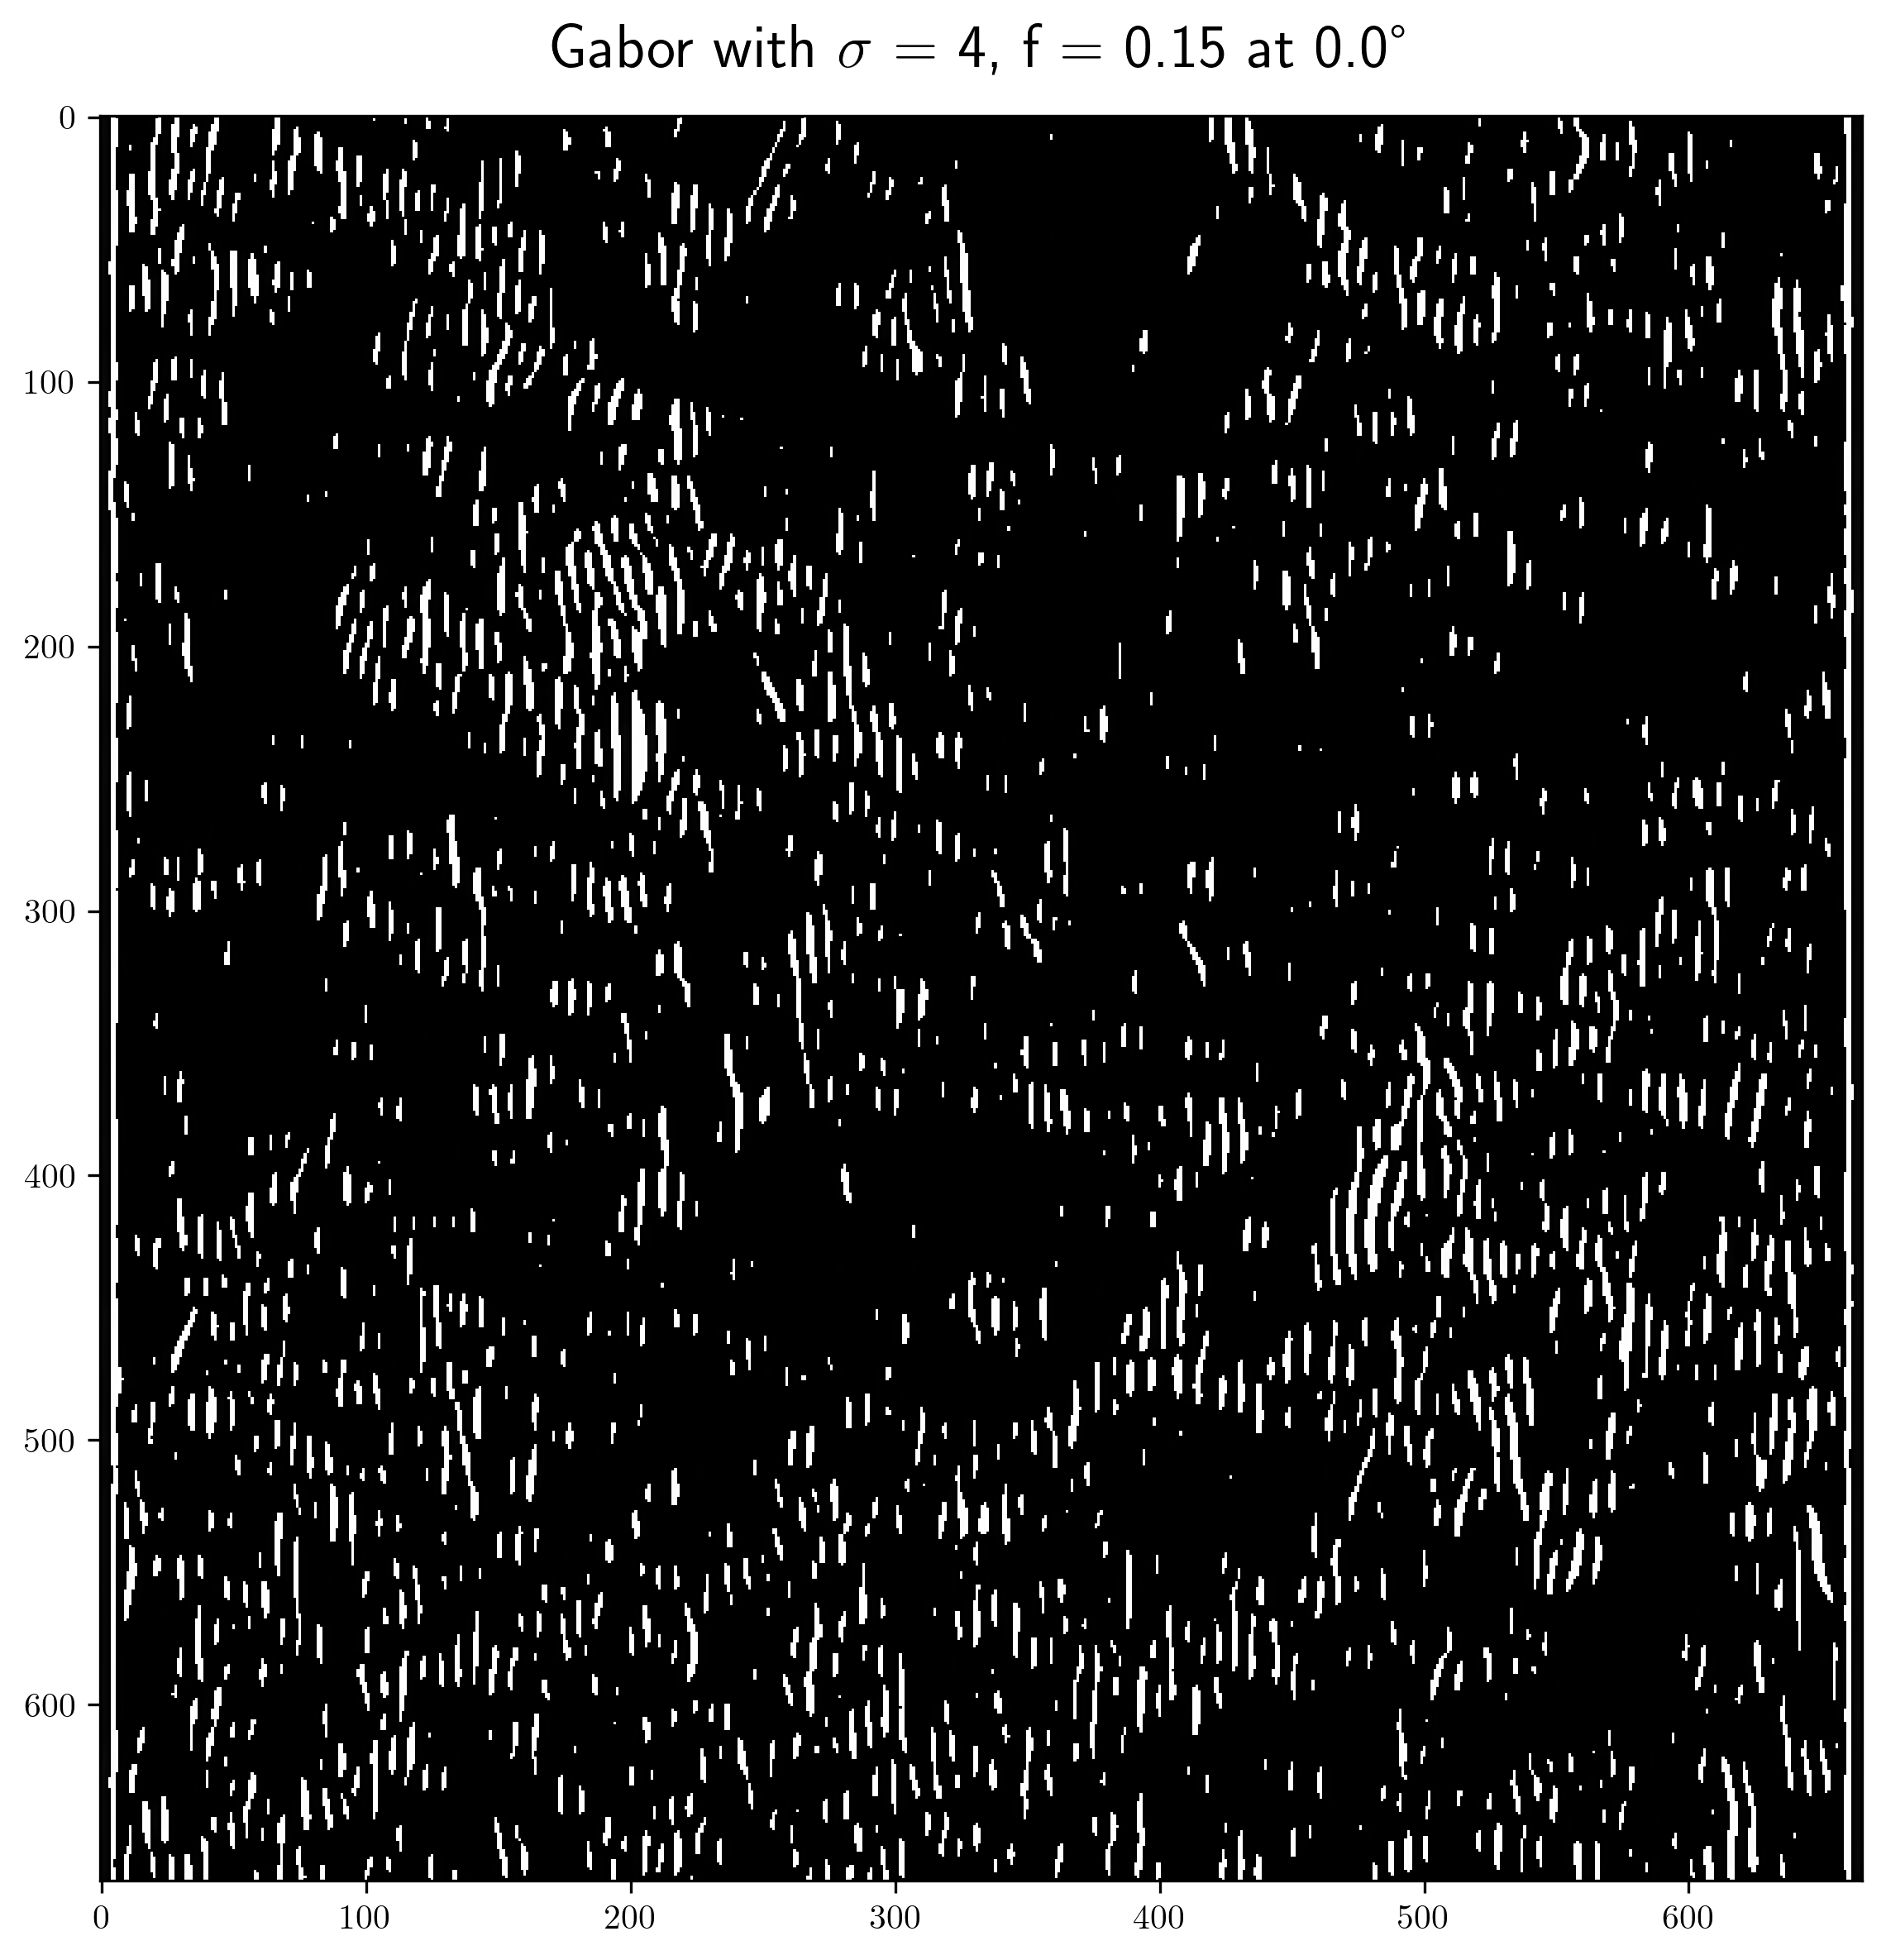
\includegraphics[width=\textwidth]{img/Features_4_015_0.png}
         \subcaption{Kernel with $\sigma$ = 4, f = 0.15 and 0 ° rotation}\label{fig:feat06}
     \end{subfigure}
        \caption{Result of convolving differently oriented gabor wavelets with an Landsat-8 image of Bremen}\label{fig:gaborExample}
    \end{figure}

%
\newpage
  \subsection{K-Means Clustering}\label{sec:kmeans}
    K-means clustering is an unsupervised learning algorithm that is used to partition $n$ observations into $k$ clusters. 
    Each observation belongs to the cluster with the nearest mean, serving as a prototype of the cluster. 
    This method has many applications in data mining, image processing, and pattern recognition.
    The algorithm consists of three steps:
    \begin{enumerate}
        \item \textbf{Initialization}: Choose $k$ initial centroids from the data points.
        \item \textbf{Assignment}: Assign each data point to the nearest centroid, forming $k$ clusters.
        \item \textbf{Update}: Recalculate the centroids as the mean of all data points in the cluster. 
    \end{enumerate}
    This process is repeated until a maximum number of iterations or minimal changes in centroids is reached~\autocite{Sinaga2020}.\\ % TODO read
    Mathematically a set of observations $(x_1, x_2, \ldots, x_n)$, where each observation is a $d$-dimensional real vector.
    K-means clustering aims to partition the $n$ observations into $k$ ($\leq n$) sets $S = \{S_1, S_2, \ldots, S_k\}$ so as to minimize the within-cluster sum of squares. \\
    The objective is to find:
    \begin{equation}
        \min{S} = \sum{i=1}^{k} \sum{x \in S_i} \| x - \mu_i \|^2
    \end{equation}
    where $\mu_i$ is the mean of points in $S_i$.
    %
    The K-Means clustering algorithm is used for surface classification using the feature enriched multi band satellite data.
    \Cref{fig:kmeansclusters} shows the result of clustering land surface types (the shown clustering did not use feature enhancement with Gabor and only used the band information as basis).%TODO fix that!  
        \begin{figure}[!htbp]
          \centering
          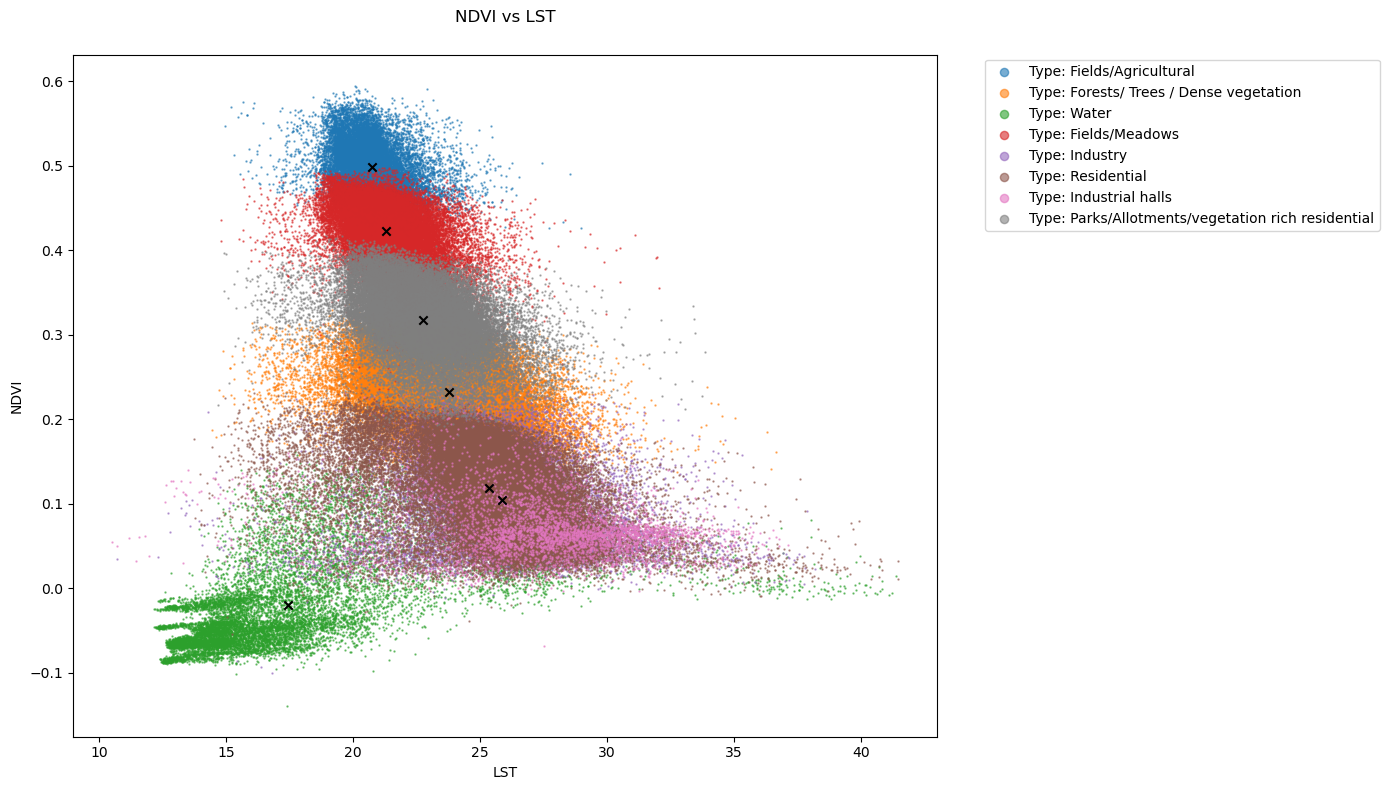
\includegraphics[width=\textwidth]{img/NDVI vs LST.png}
          \caption{Result of clustering (coloured dots) plotted as \gls{NDVI} value and \gls{LST}\label{fig:kmeansclusters}}
        \end{figure}

    The pre-trained model is stored to disk and can be used to classify similar images again. 
    Since the class labels are not consistently applied, the labels need to be reassigned to the correct cluster.
    For this the cluster-centres of the clusters from the trained K-Means are saved as a array n-tuples for each class, where n is the number of features used for training.
    \newpage
    \subsubsection{Label Reassignment}
    The distance from the cluster centres of the initial training dataset and the centres of the newly classified data is calculated. 
    To get consistent mapping of class names to classification id, the minimal distance is not sufficient since a assignment of multiple classes to one original class be minimal. 
    To mitigate this issue a \textit{Hungarian Algorithm} is used, minimizing an overlying metric and creating a bijective assignment. 
    The distances are then minimized using the sum of distances of all cluster centres as optimization metric.
      \begin{equation}
        \min = \sum{i}\sum{j} C_{i,j}X_{i,j}
      \end{equation}
  % \subsection{Random Forest Algorithm}\label{sec:randomForrest}
    %   Random Forest is a versatile ensemble learning method widely used in machine learning for both classification and regression tasks.
    %   It operates by constructing multiple decision trees during the training phase and outputting the mode of the classes (in classification) or mean prediction (in regression) of the individual trees.
    %   This method is particularly noted for its robustness and ability to handle large datasets with complex structures.
    %   
    %   The algorithm involves creating multiple decision trees using bootstrap aggregating, where each tree is trained on a random subset of the data with replacement, and at each node, a random subset of features is chosen for splitting.
    %   The ensemble approach mitigates the risk of overfitting, a common problem in individual decision trees, making Random Forest an effective tool even in scenarios with noisy or incomplete data. 
    %   In the Land Cover use case, this should increase robustness against seasonal variability of surface type appeal and changes due to variation in local climate and geology.\\ \\
    %   
    %   One of the strengths of Random Forest lies in its capacity to provides a measure of feature importance, which is valuable for understanding the driving factors in a model and provides a point for further optimization in case the performance is not sufficient.
    %   The downsides of the algorithm is, that it is computationally intensive, especially with a large number of trees, and the resultant model can be less interpretable compared to simpler models like linear regression or single decision trees.\\
    %   
    %   In practical applications, Random Forest has been employed across various domains, ranging from predictive analytics in finance (e.g.\ in~\autocite{Zhang2022}) and healthcare (e.g.~\cite{Kane2014}) and natural language processing. 
    %   It is suitable for usage in time line analysis and was used in this application for predicting the surface types based on the imagery which has been show to be effective in the past in~\autocite{Piao2021}.
    %   %
    %   Its ability to provide robust and accurate predictions even in the presence of complex data interactions has cemented its place as a staple algorithm in the machine learning toolkit.
    
\newpage
\section{Comparable Definition of Urban Heat Islands}\label{sec:definition}
    \subsection{Introduction}
      The definitions of \glspl{SUHI} in the literature are varying slightly and do not take into account that, most definitions do not allow easy comparison between different areas or times.
      Local studies often use a single reference measurement station and use the absolute temperature difference as a measure of intensity.
      Other use the surface temperature of surrounding rural areas like forests as a reference% (e.g.TODO add sources, maybe add examples? 
      The definition of the U.S.~EPA (~\cite{EPA2008}) and the German Weather Service (\gls{DWD}) both define it as an feature defined by increased temperature between the urbanized areas compared to the surrounding.\\ 
      Different studies analysing \glspl{UHI} use difference reference temperatures.
      The first goal of this work is defining a systematic reproducible approach to measure \gls{UHI} intensity.
%
    \subsection{Approach}
    As a starting point the method of~\cite{Sobrino2020} was adapted, where \gls{SUHI} where compared in different cities around the world using Sentinel-3 images. 
    For each city a buffer zone was calculated around the city border, using the average temperatures of the different areas as a comparison point.
    This was then used to identify and measure the intensity of the heat islands within the city area.\\ 
    This work uses the same basic approach but Landsat 8/9 data was used and combined with different \gls{ML} techniques for surface classification (see \cref{sec:classification}). 
    In~\cite{Sobrino2020} urban adjacent, future urban adjacent and peri-urban areas are defined as buffers.
    These where adapted by removing the urban growth projection (since the scope of the paper was the investigation of \glspl{SUHI} in 2050 that does not match the goal for this work).
    The urban area is identified by detecting land cover classes indicating a larger area of build up classes. 
    These Areas are then converted into a polygon that are extended by buffer zones as shown in \cref{fig:bufferedBremen}.
    Additionally an approach is discussed where the relative (statistical) intensity is used compared to the absolute temperature difference to compensate for seasonal temperature spread within certain areas.
    \subsection{Definition of Urban Heat Islands}\label{sec:definition}
    The following \gls{UHI} definition is proposed and used throughout this document.\\
    \\
    \noindent\fcolorbox{gray!30}{gray!40}{%
      \parbox{\linewidth}{%
      An \gls{SUHI} is an area with increased surface temperature within an urban space, where the temperature is at least 2 standard deviations above the average temperature of the urban adjacent rural buffer zone, corrected for larger settlements.\\ }}\vspace{2cm}
% 
    For comparability a statistical metric is used, since the absolute intensity as well as the daily temperature spread varies with the seasons %TODO source
    and is easily altered by water bodies or other thermal masses in the image.\\ 
    
    The proposed threshold of at least two standard deviations above the average temperature was chosen since this gave consistent results over the seasons. %TODO verify!
    The reference measurement is done using the surface temperature of the peri-urban buffer zone and removing all larger urban areas within it. 
    This will get rid of other cities or larger industrial sides close to the area of interest.
    The mean temperature and variation within the peri-urban area is then calculated and used as reference.
    % Assuming that temperature is normal distributed the temperature should lie outside of the 95%ile 
    Depending on season the temperature distribution will vary, due to the definition using the standard deviation the detection of \glspl{UHI} is coupled to the range of temperatures observed within the image. 
    During processing single outlier areas as well as clouds, cloud shadows are removed and holes within the urban area are closed, this allows to include parks and other urban green areas to be processed and only includes larger areas of elevated temperatures as urban heat islands. 
    This will increase robustness of \gls{UHI} detection to reduce the influence of single hot surfaces (such as solar panels or industrial tanks) during detection.
    % TODO normal dist? 
   %TODO IMAGES for each step / marked with temps to make it easier to understand  

    \subsubsection{Urban Buffer Zones}\label{sec:urbanBufferzone}
      To generate the different temperature statistics buffer zones must be created, to do this multiple areas are defined using \cref{equ:areas}.
%
      \begin{equation}\label{equ:areas}
	      W_U = \frac{A_U^{\frac{1}{2}}}{4}
	      W_P = \frac{6\cdot A_U^{(\frac{1}{2}-W_U)}}{4}
      \end{equation}
      Where $W_U$ is the urban and suburban area (the urban area and a suburban buffer zone) and $W_P$ the peri-urban area.
      These definitions where used in~\cite{Sobrino2020} and were developed in the 90s for urban development (\cite{AlkanBala2014}).
      The practical implementation was done as part of the classification and is described in \cref{sec:urbanAreaExtraction}. \\
      The heat island is then defined as area that is more then $3\times \sigma$ above the mean temperature of the surrounding area $W_P$, while the surrounding area is defined as a fixed buffer based on the size of the urban area and clean the area of larger settlements. 
      \begin{figure}
        \includegraphics[width=\textwidth]{img/UrbanAreaBremen}
        \caption{Urban Area of Bremen, with buffer zones for Adjacent and Peri Urban Area\label{fig:bufferedBremen}}
      \end{figure}
%
    \subsection{Conclusions}
    The definition of \glspl{UHI} using reference regions and a statistical threshold for identifying areas is a methodology that has multiple advantages compared to using absolute values and single reference points. 
    The impact of seasonal and geographic variations in temperature spread as well as weather and other metrological effects are reduced, since the peri urban area has a mixed composition. 
    % TODO link to the findings later 
    % TODO expand

\newpage
\section{Impact of Land Cover Changes on Urban Heat Islands}\label{sec:LULC}
    \subsection{Introduction}
      One of the key factors influencing the intensity and distribution of \glspl{UHI} is land cover change, primarily driven by urbanization and associated human activities.
      Soil properties impact the emissivity, thermal conductivity and heat capacity of an area and increases in build up reduce surface water availability. 
      \\    
      This section looks into the relationship between land cover change and \glspl{UHI} effects using \gls{LULC} detection based on the previously classified Landsat images.
      The exploration begins with an overview of the impact of land cover changes and the underlying mechanisms on Urban heat islands and highlighting the critical role that changes in land cover play in modulating urban thermal environments.
      The discussion extends to the various types of land cover alterations, such as the replacement of natural landscapes with built-up areas, deforestation, and changes in vegetation cover, and how these modifications contribute to the exacerbation or mitigation of \glspl{UHI}.
      \\
      Furthermore, the chapter examines the multi-dimensional impact of \glspl{UHI} under the lens of land cover change.
      This includes the analysis of spatial and temporal patterns of \glspl{UHI}, the influence of different urban forms and structures, and the effectiveness of various mitigation strategies, such as urban greenery and reflective materials in buildings and pavements.
      \\
      Through a synthesis of current research findings and case studies, this chapter aims to provide a comprehensive understanding of the dynamics between land cover change and \glspl{UHI}.
      It also seeks to offer insights into sustainable urban planning and design practices that can mitigate the adverse effects of \glspl{UHI}, thereby contributing to the development of more liveable and resilient urban environments.
%
    \subsection{Impact of Land cover/ Surface type on Heat Build-up}
      The change of the urban surface properties is one of the major factors causing \glspl{SUHI}.  
      Multiple studies have shown that land cover has a significant impact on land surface temperature and \glspl{UHI} (e.g.~\autocite{Karakus2019},~\cite{Weng2004} and~\cite{Stewart2011})
      %
    \subsubsection{Classification }\label{sec:classification}
      The methodology employed for land cover classification involved the multi-step process utilizing satellite imagery, feature enhancement and machine learning techniques shown in \cref{fig:pipeline} and described in \cref{sec:pipeline}.
      The primary data source was 11-band Landsat images, which provided a comprehensive spectral view of the area to be classified.
      To augment the dataset and enhance the classification accuracy, Gabor filtering (see \cref{sec:gabor}) was applied to the Landsat images.
      As input, the gabor filtered multispectral data of at least two different satellite images was used.
      The multi band image was loaded and cut to match the study area. 
      \begin{wrapfigure}{r}{0.4\textwidth}
       \begin{center}
         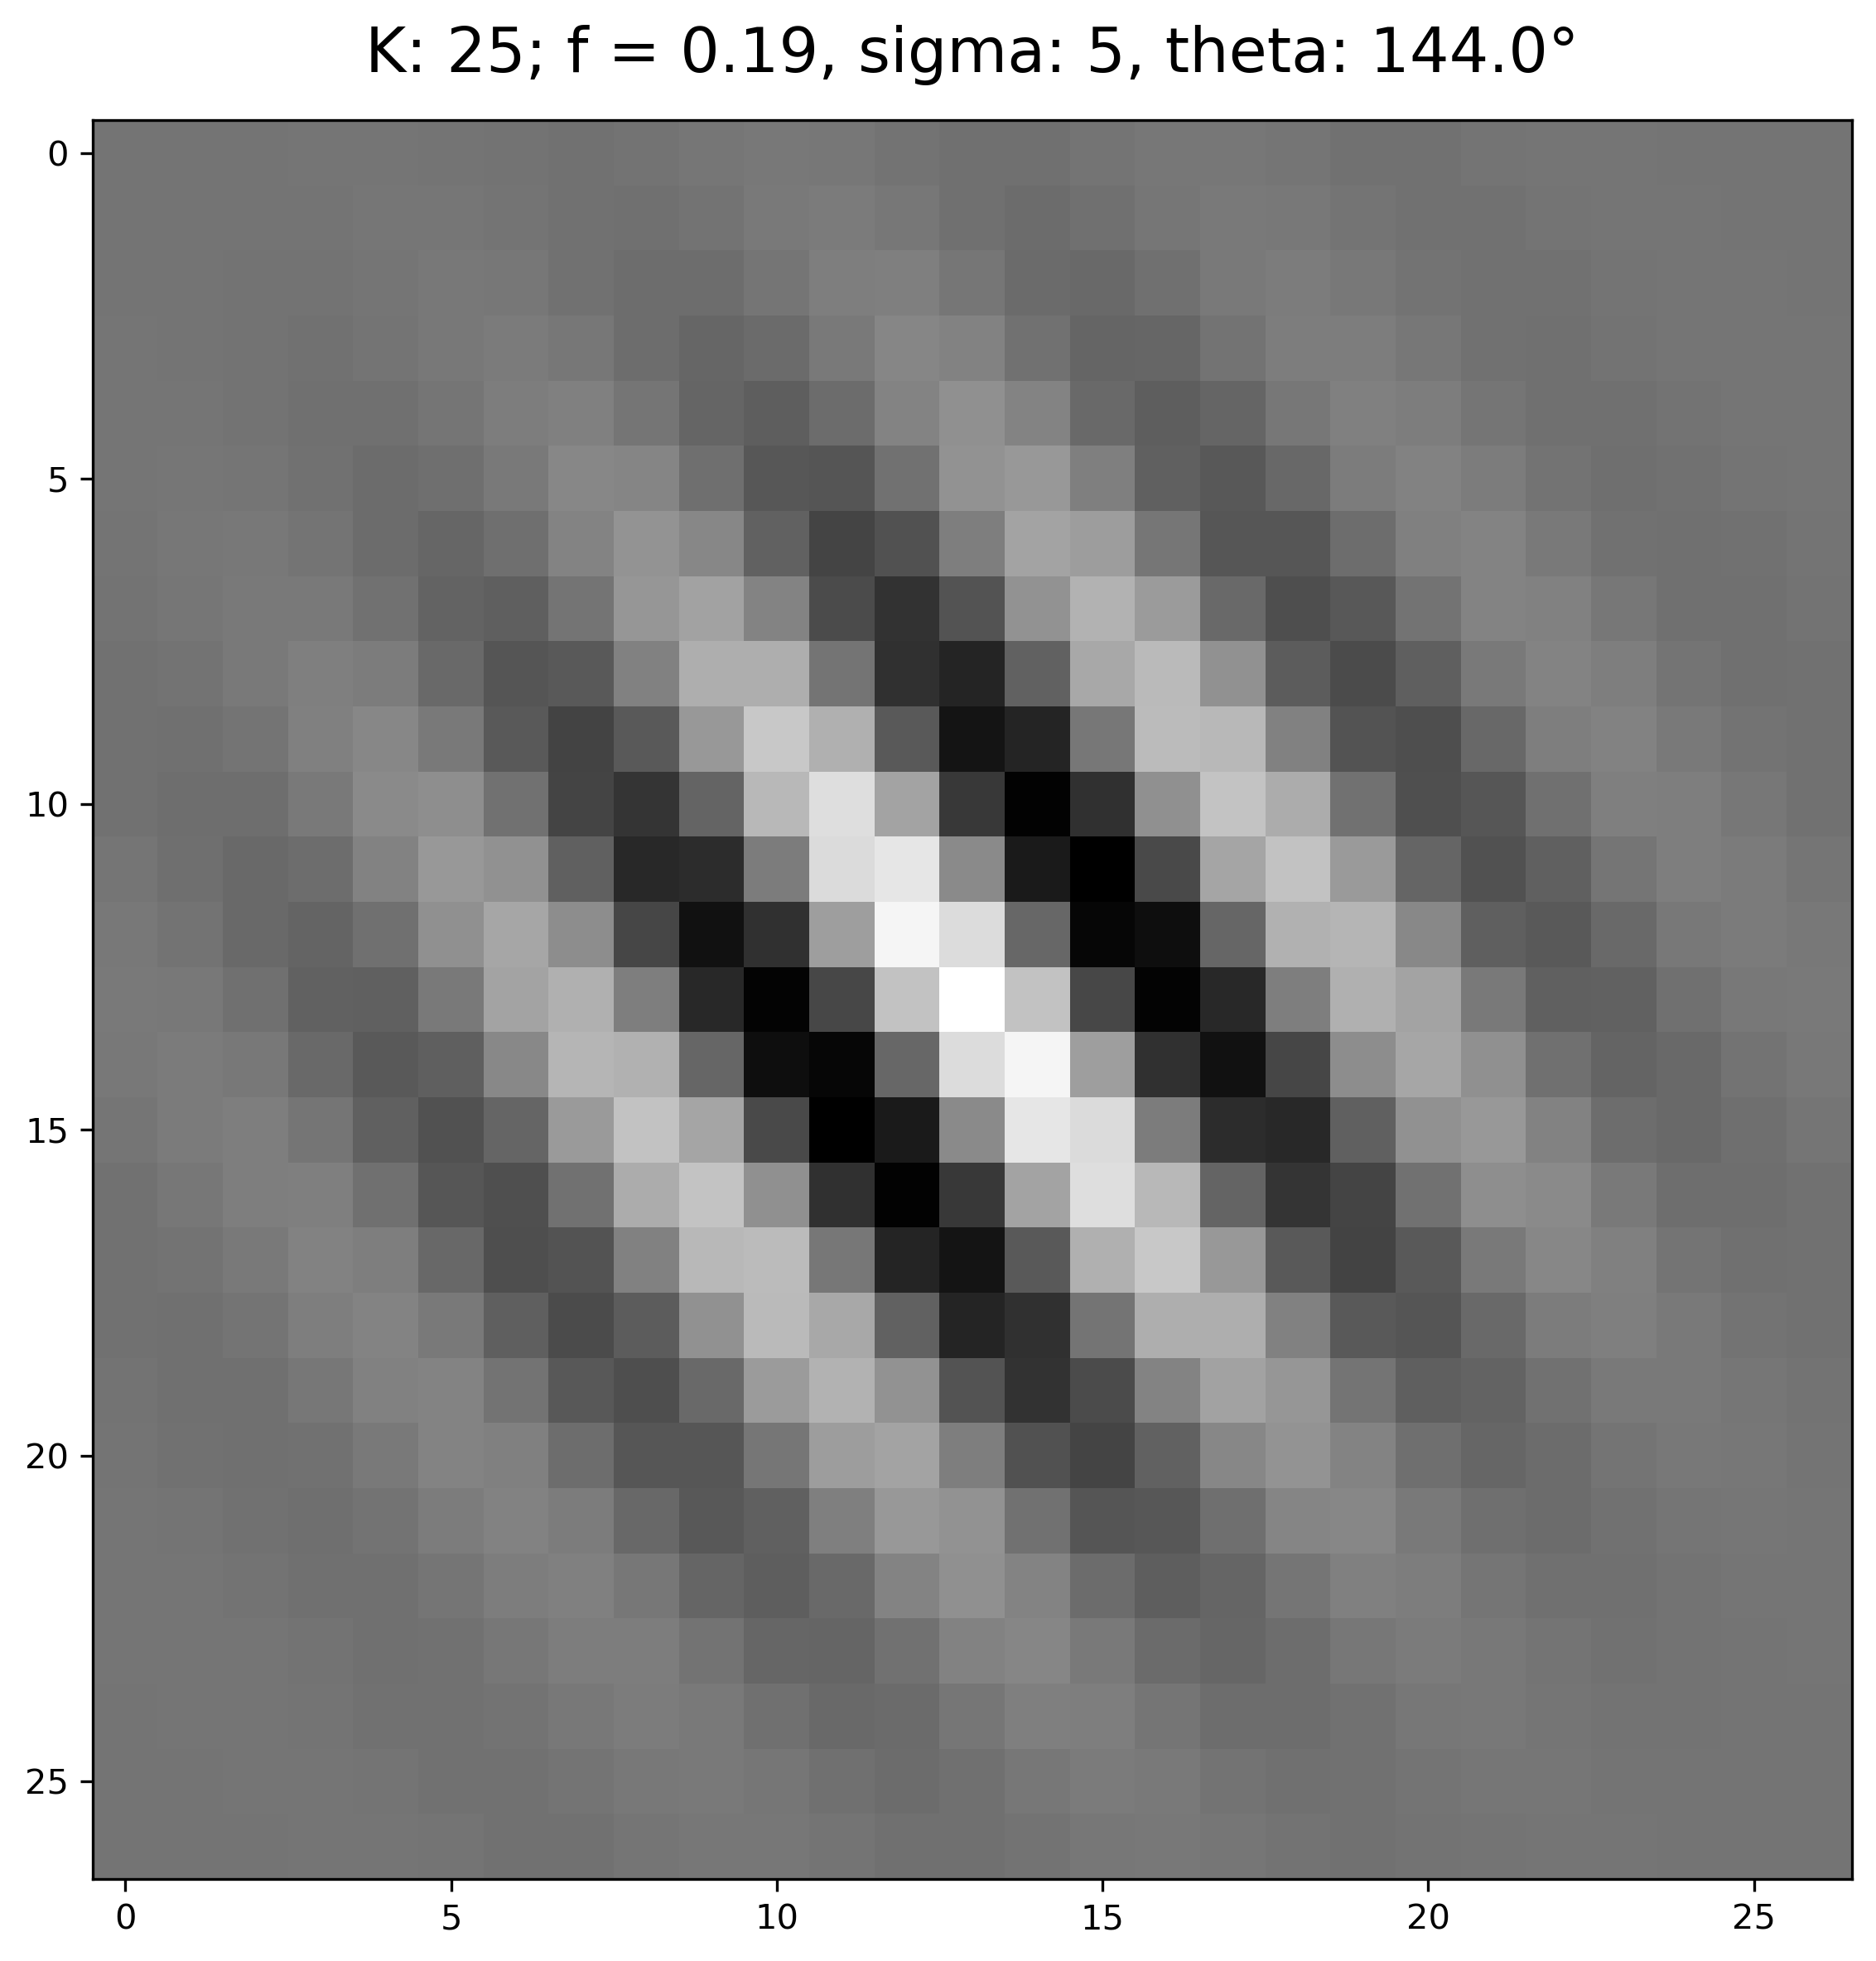
\includegraphics[width=0.4\textwidth]{img/KLarge.png}
       \end{center}
       \caption{Example Kernel for a larger kernel with 26 $\times$ 26 Pixel kernel size and multiple repetitions of the sine component}\label{fig:largeKernel}
      \end{wrapfigure}
    The analysis used the following parameters: 
      % Classification: 
    The Gabor filter was varied using different $\sigma$, $\theta$ and $f$ values.
    Due to computational restrictions the number of rotations ($\theta$) was limited to 5, a value of 4 resulted in better results. 
    For $\sigma > 2$ the classification degraded showing stripes very large patterns were detected, a value of $\sigma = 1$ resulted in a kernel size of 7 $\times$ 7 pixel and good results.
%
%    
    The usable frequencies are limited by the size of the kernel and the image resolution shown in \cref{fig:largeKernel}.
    Due to the low resolution, a large kernel size would detect features that are repeated with a features size in the range of 200 m that do not occur in large quantities in urban areas. 
    Larger kernel size with higher frequencies would increase detection capability for images with higher resolution. 
    \Cref{fig:gaborbank} shows the used kernels.
     %Due to the low resolution of 30 m per pixel high frequencies where not abl
%
    \begin{figure}[!htbp]
      \centering
      \begin{subfigure}[b]{0.3\textwidth}
        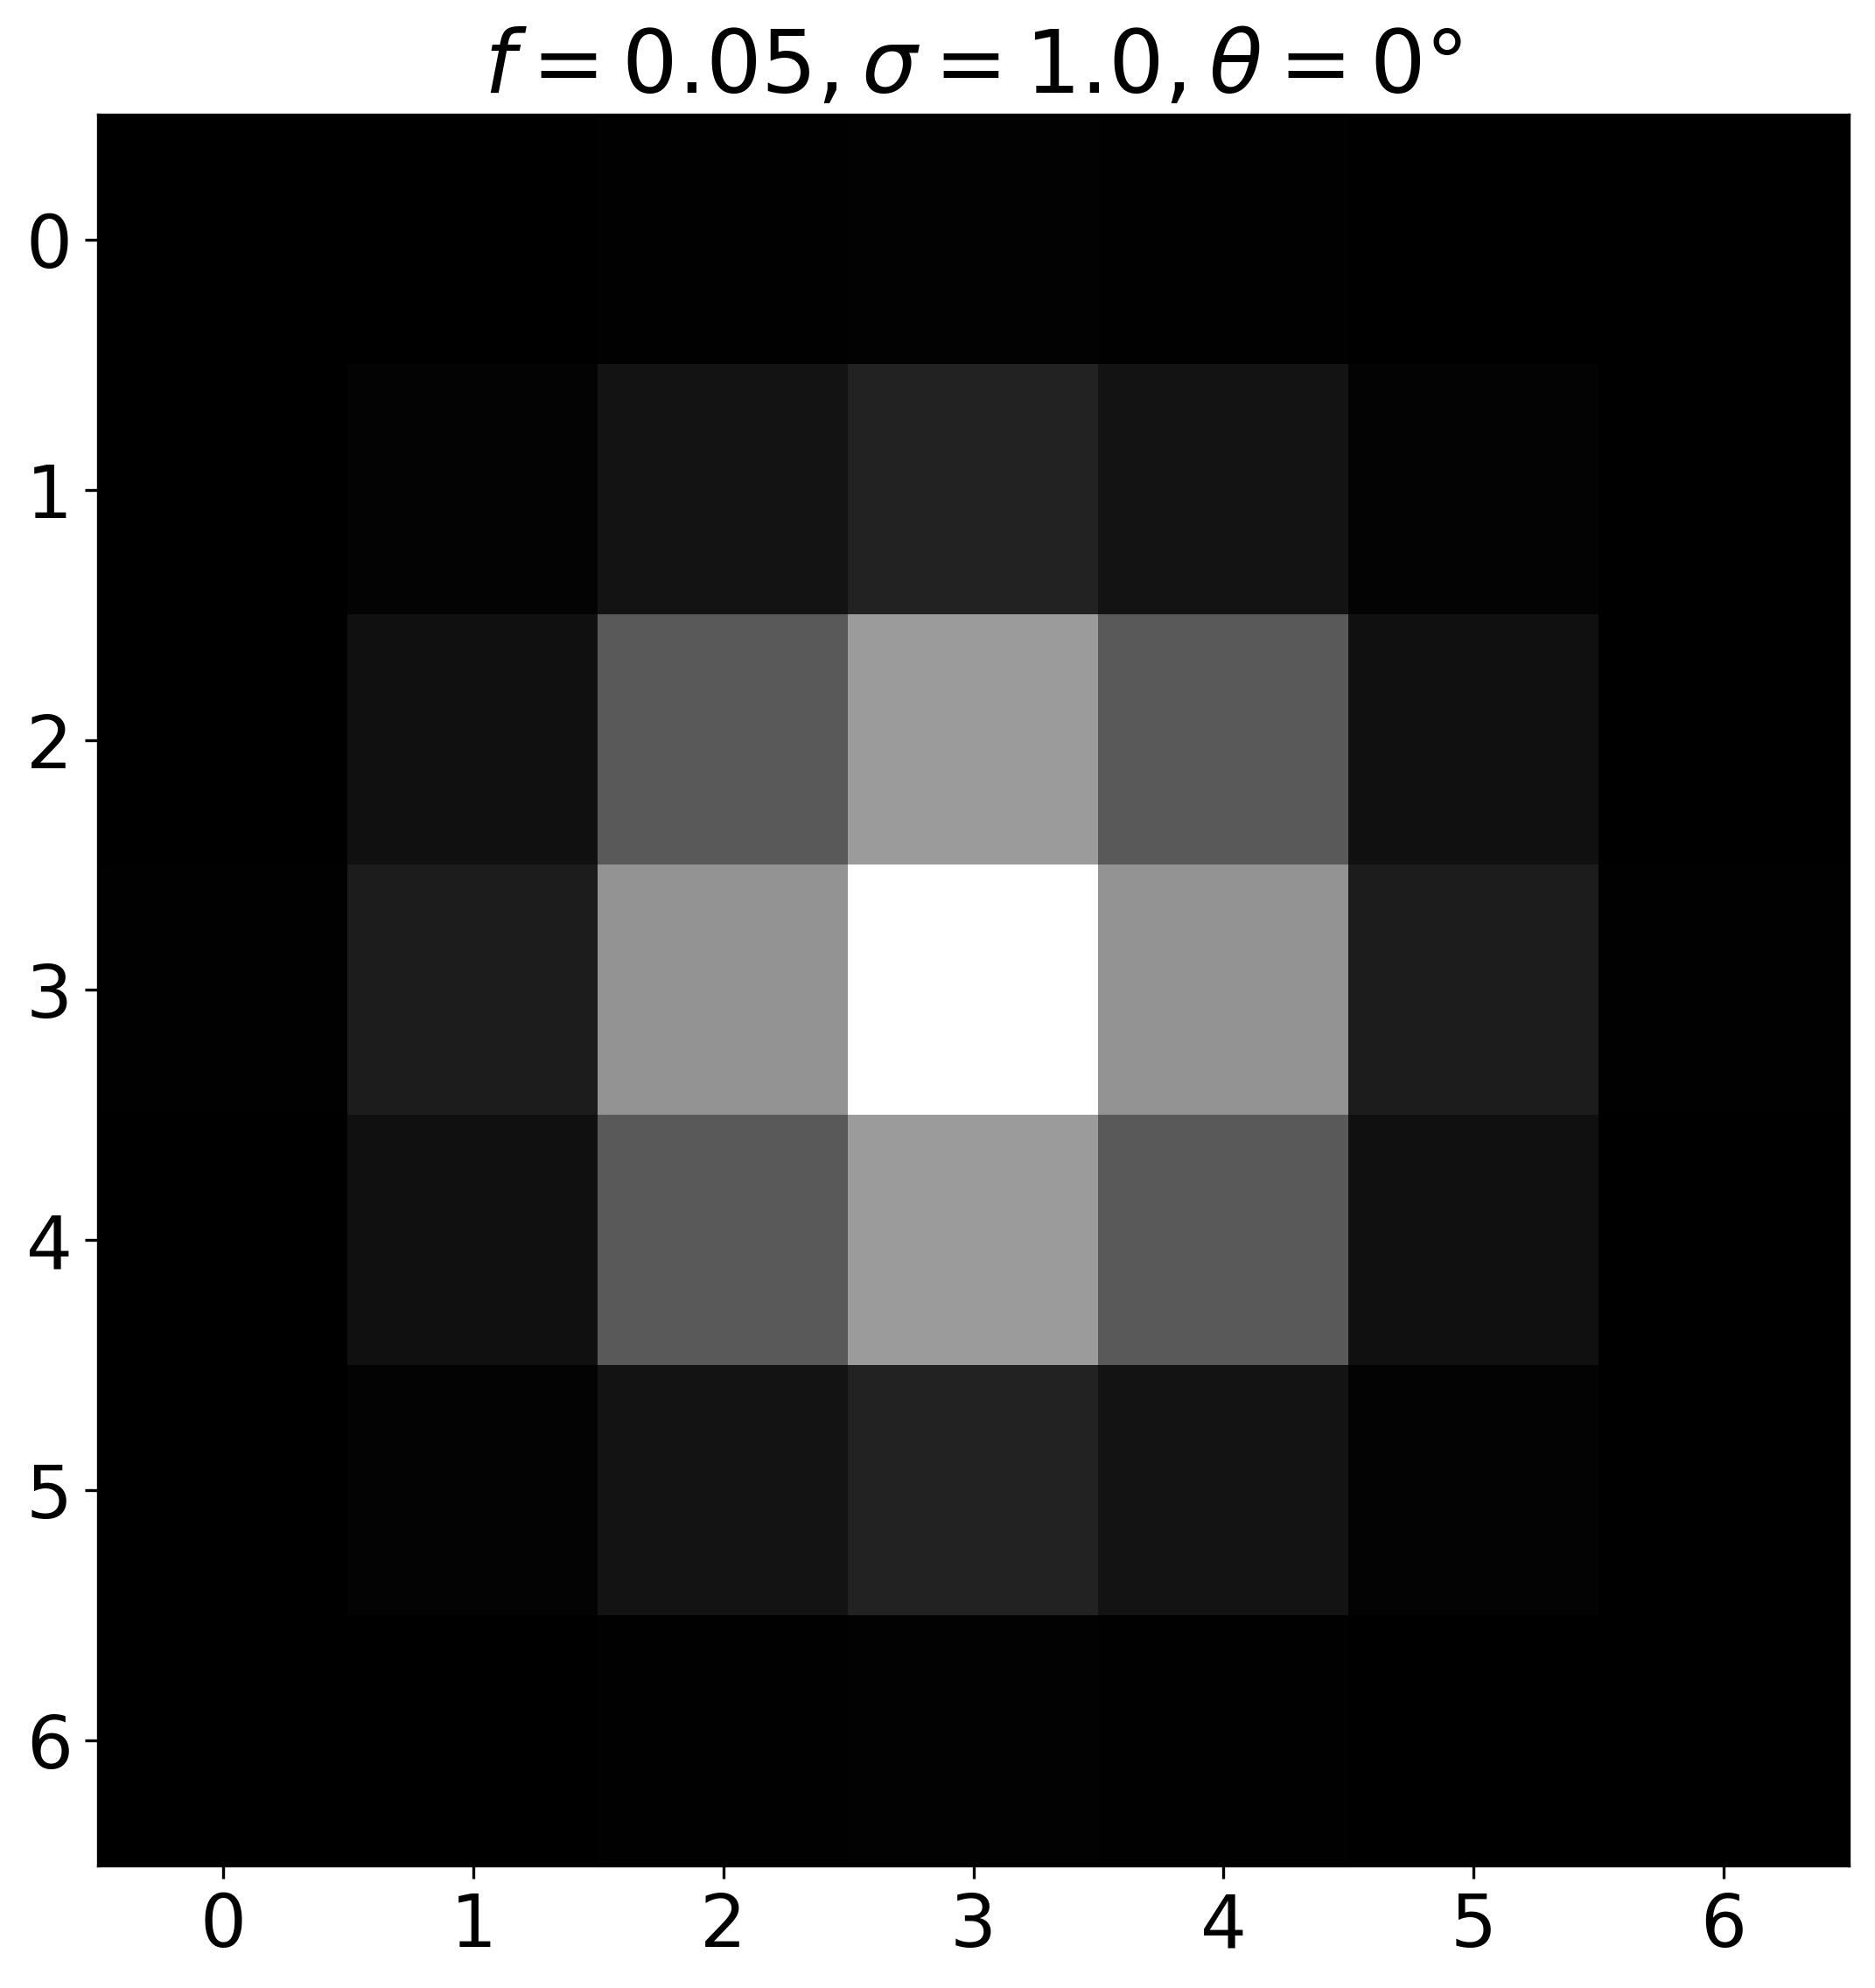
\includegraphics[width=\textwidth]{img/K0.png}
        \subcaption{Kernel 1}
      \end{subfigure}
      \begin{subfigure}[b]{0.3\textwidth}
        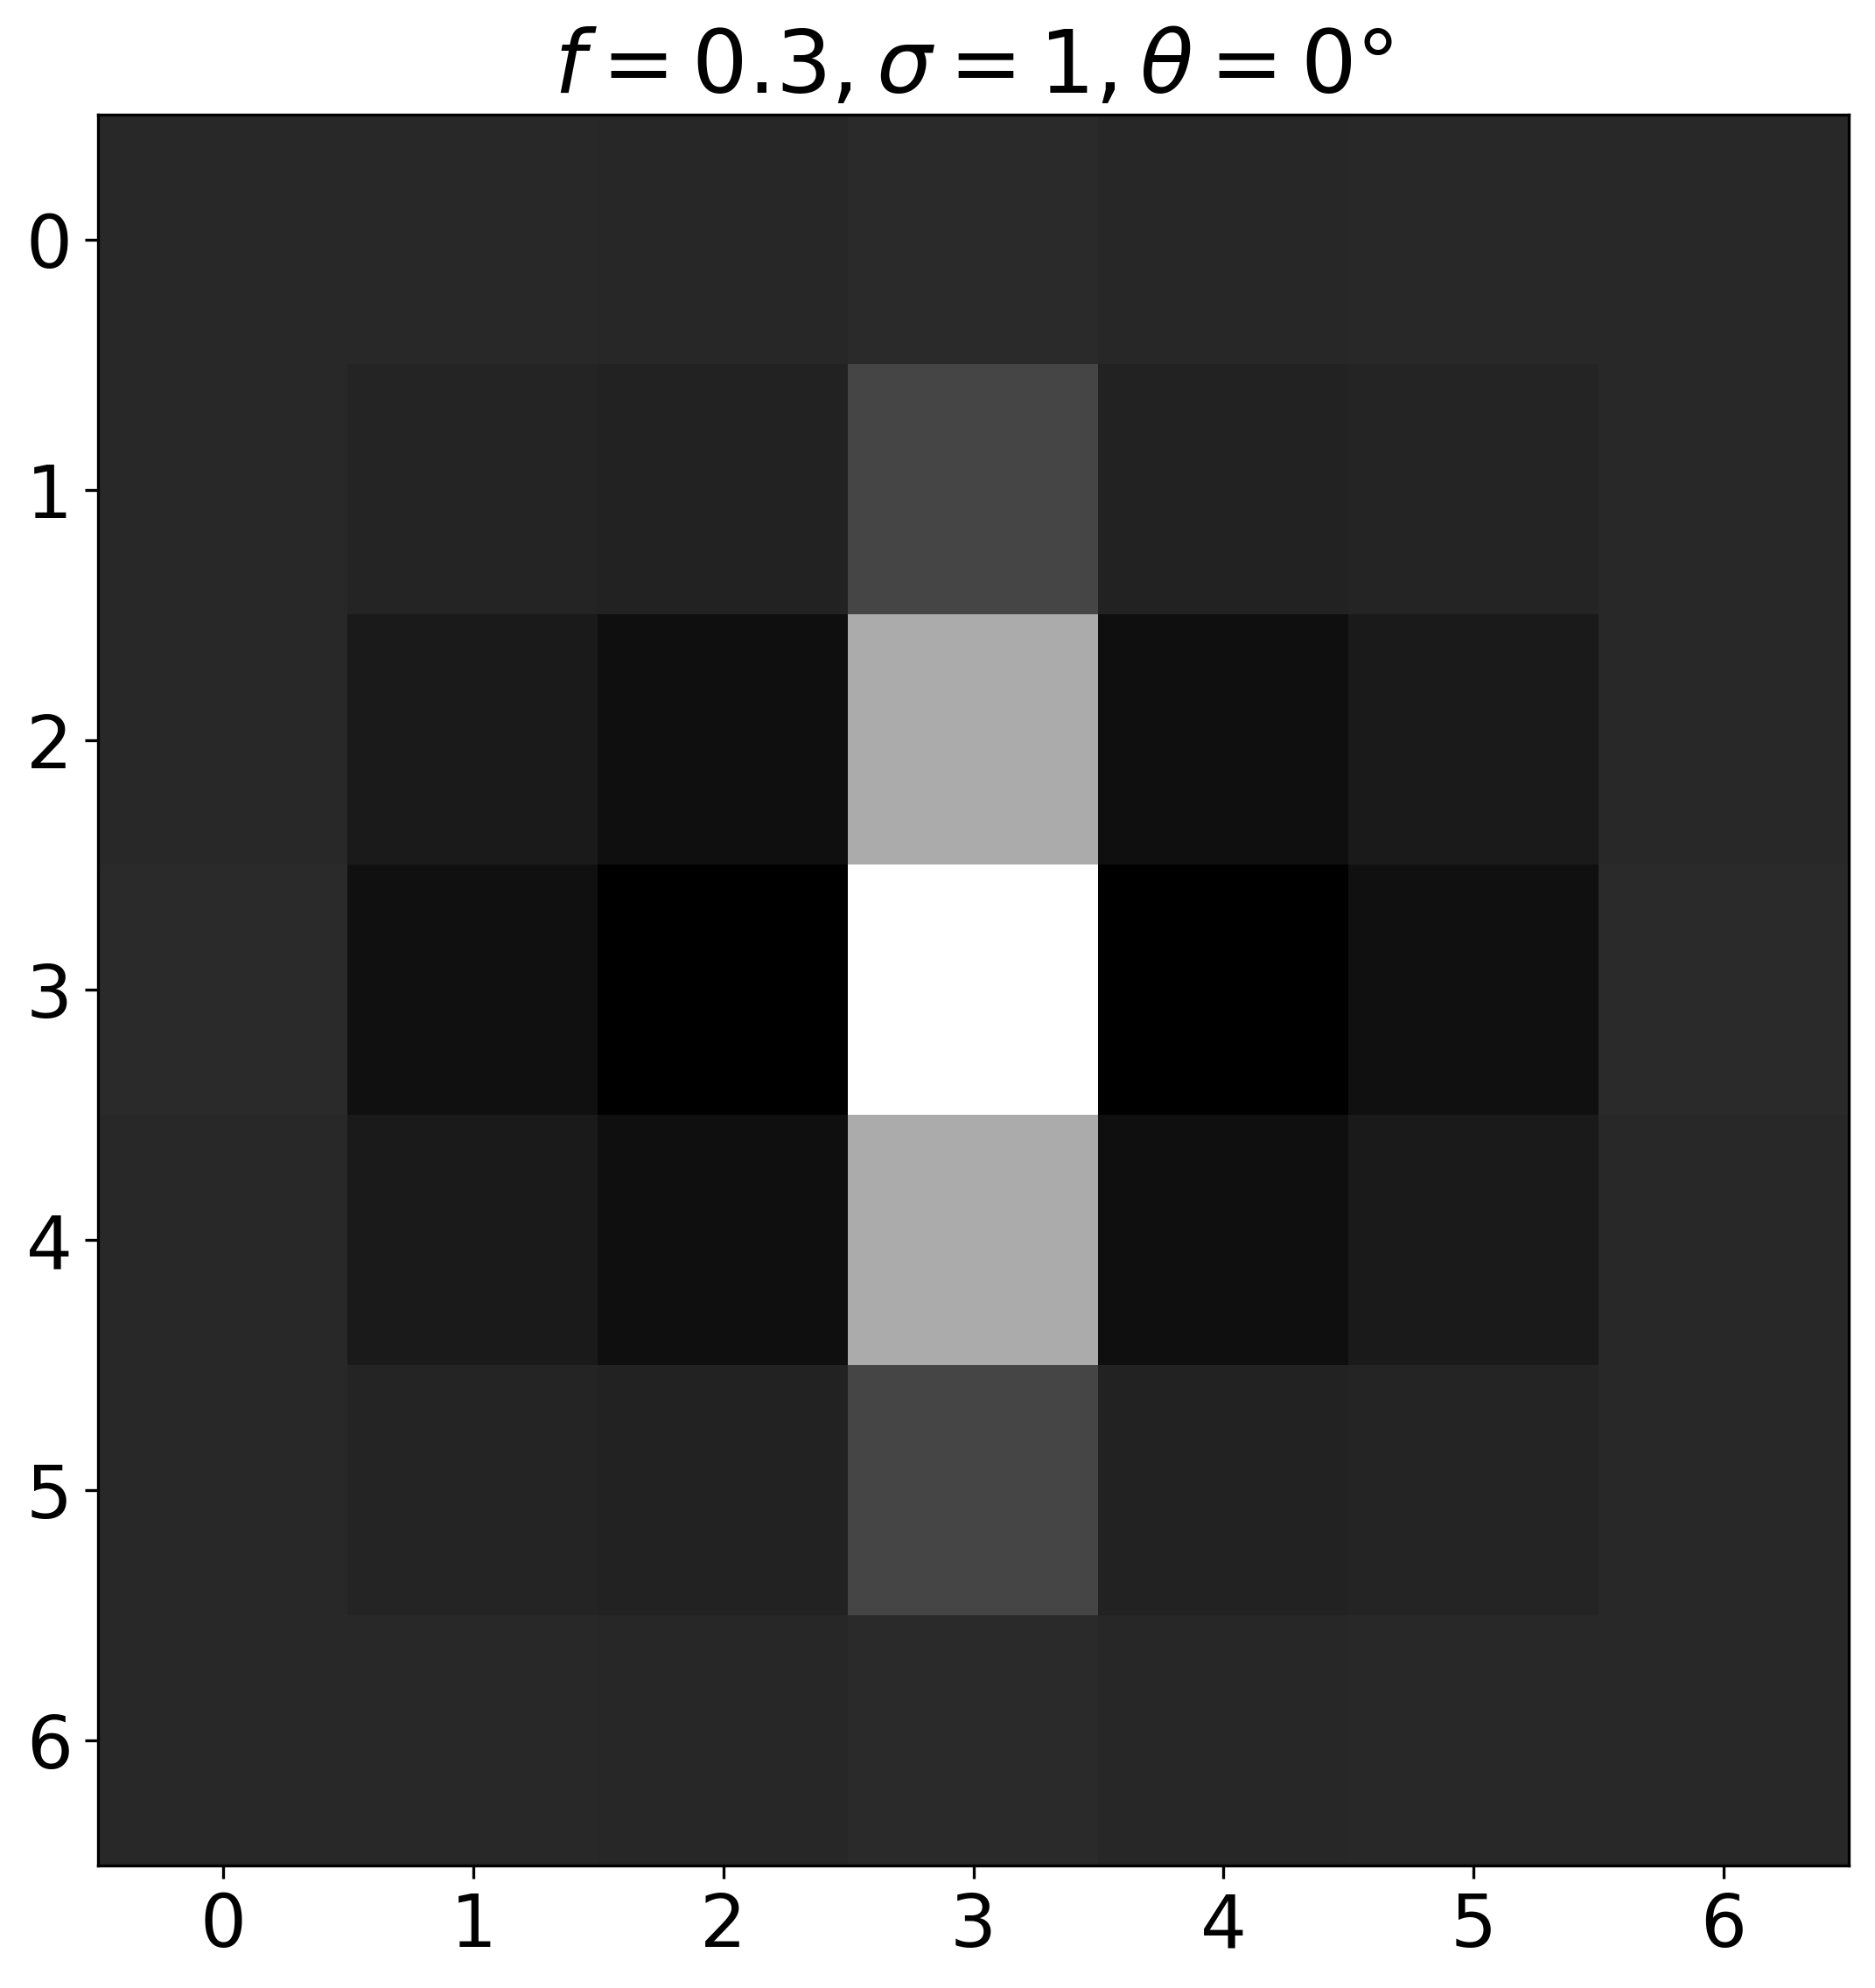
\includegraphics[width=\textwidth]{img/K1.png}
        \subcaption{Kernel 2}
      \end{subfigure}
      \begin{subfigure}[b]{0.3\textwidth}
        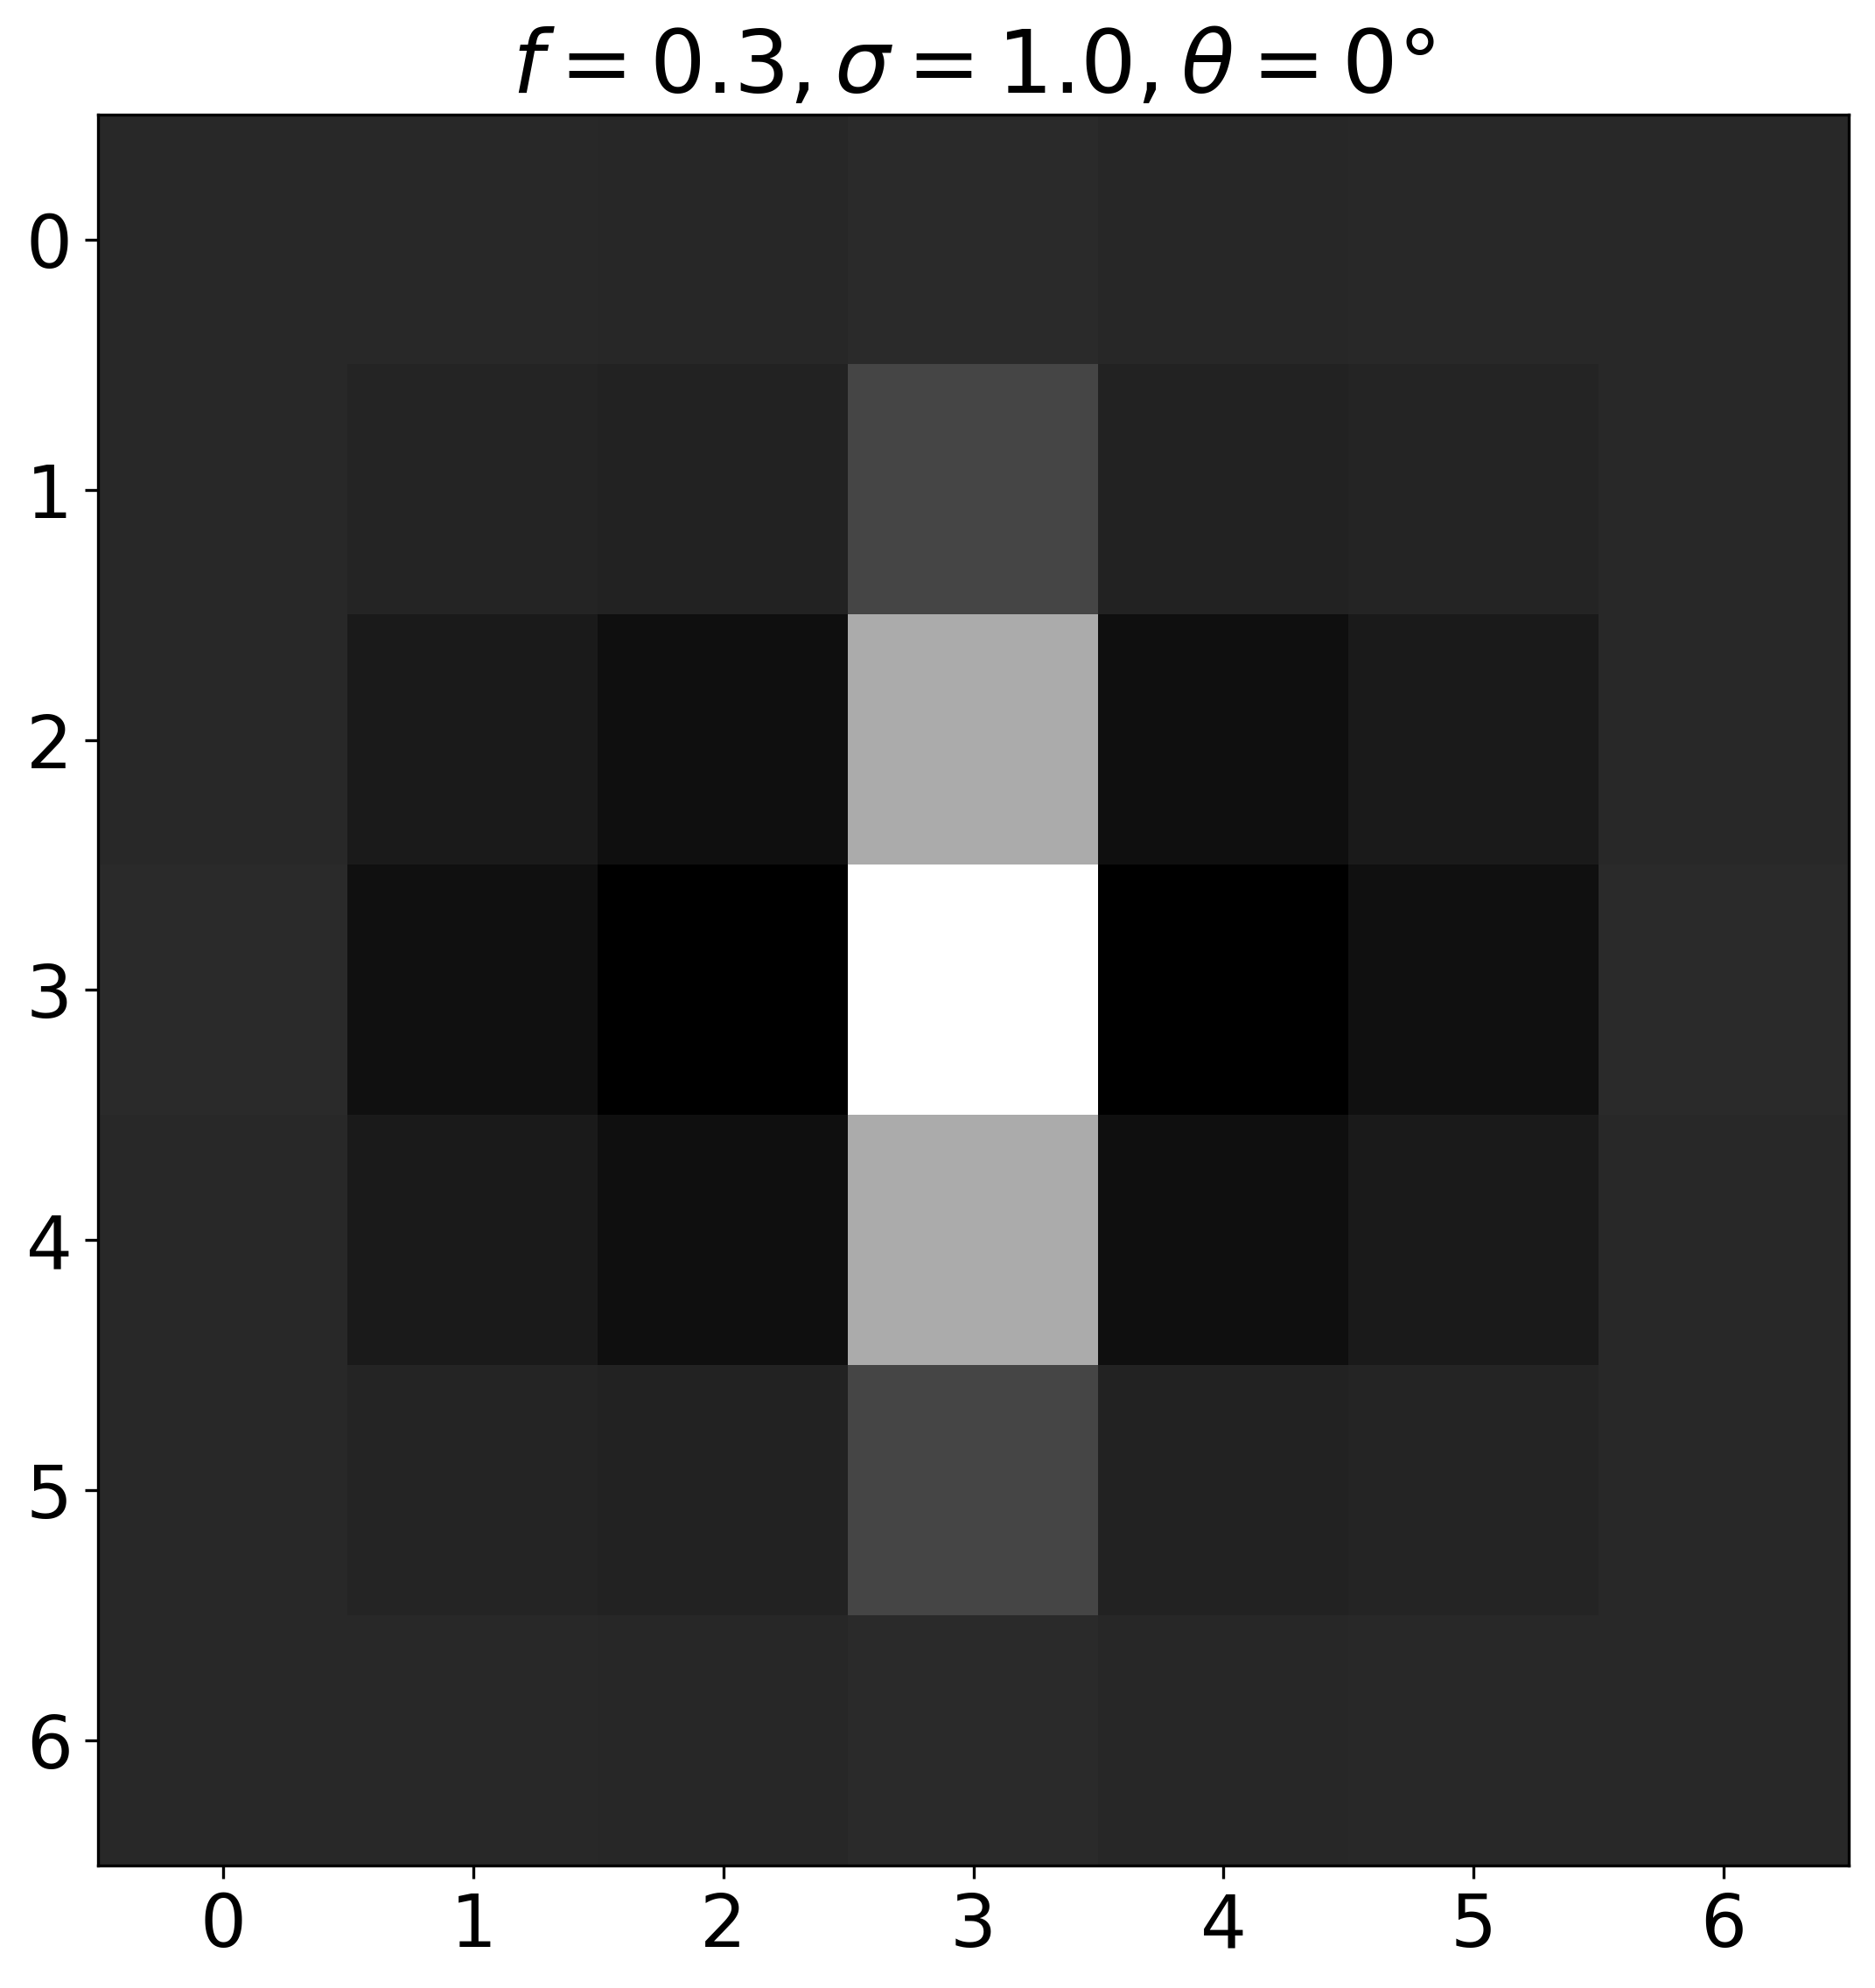
\includegraphics[width=\textwidth]{img/K2.png}
        \subcaption{Kernel 3}
      \end{subfigure}

      \begin{subfigure}[b]{0.3\textwidth}
        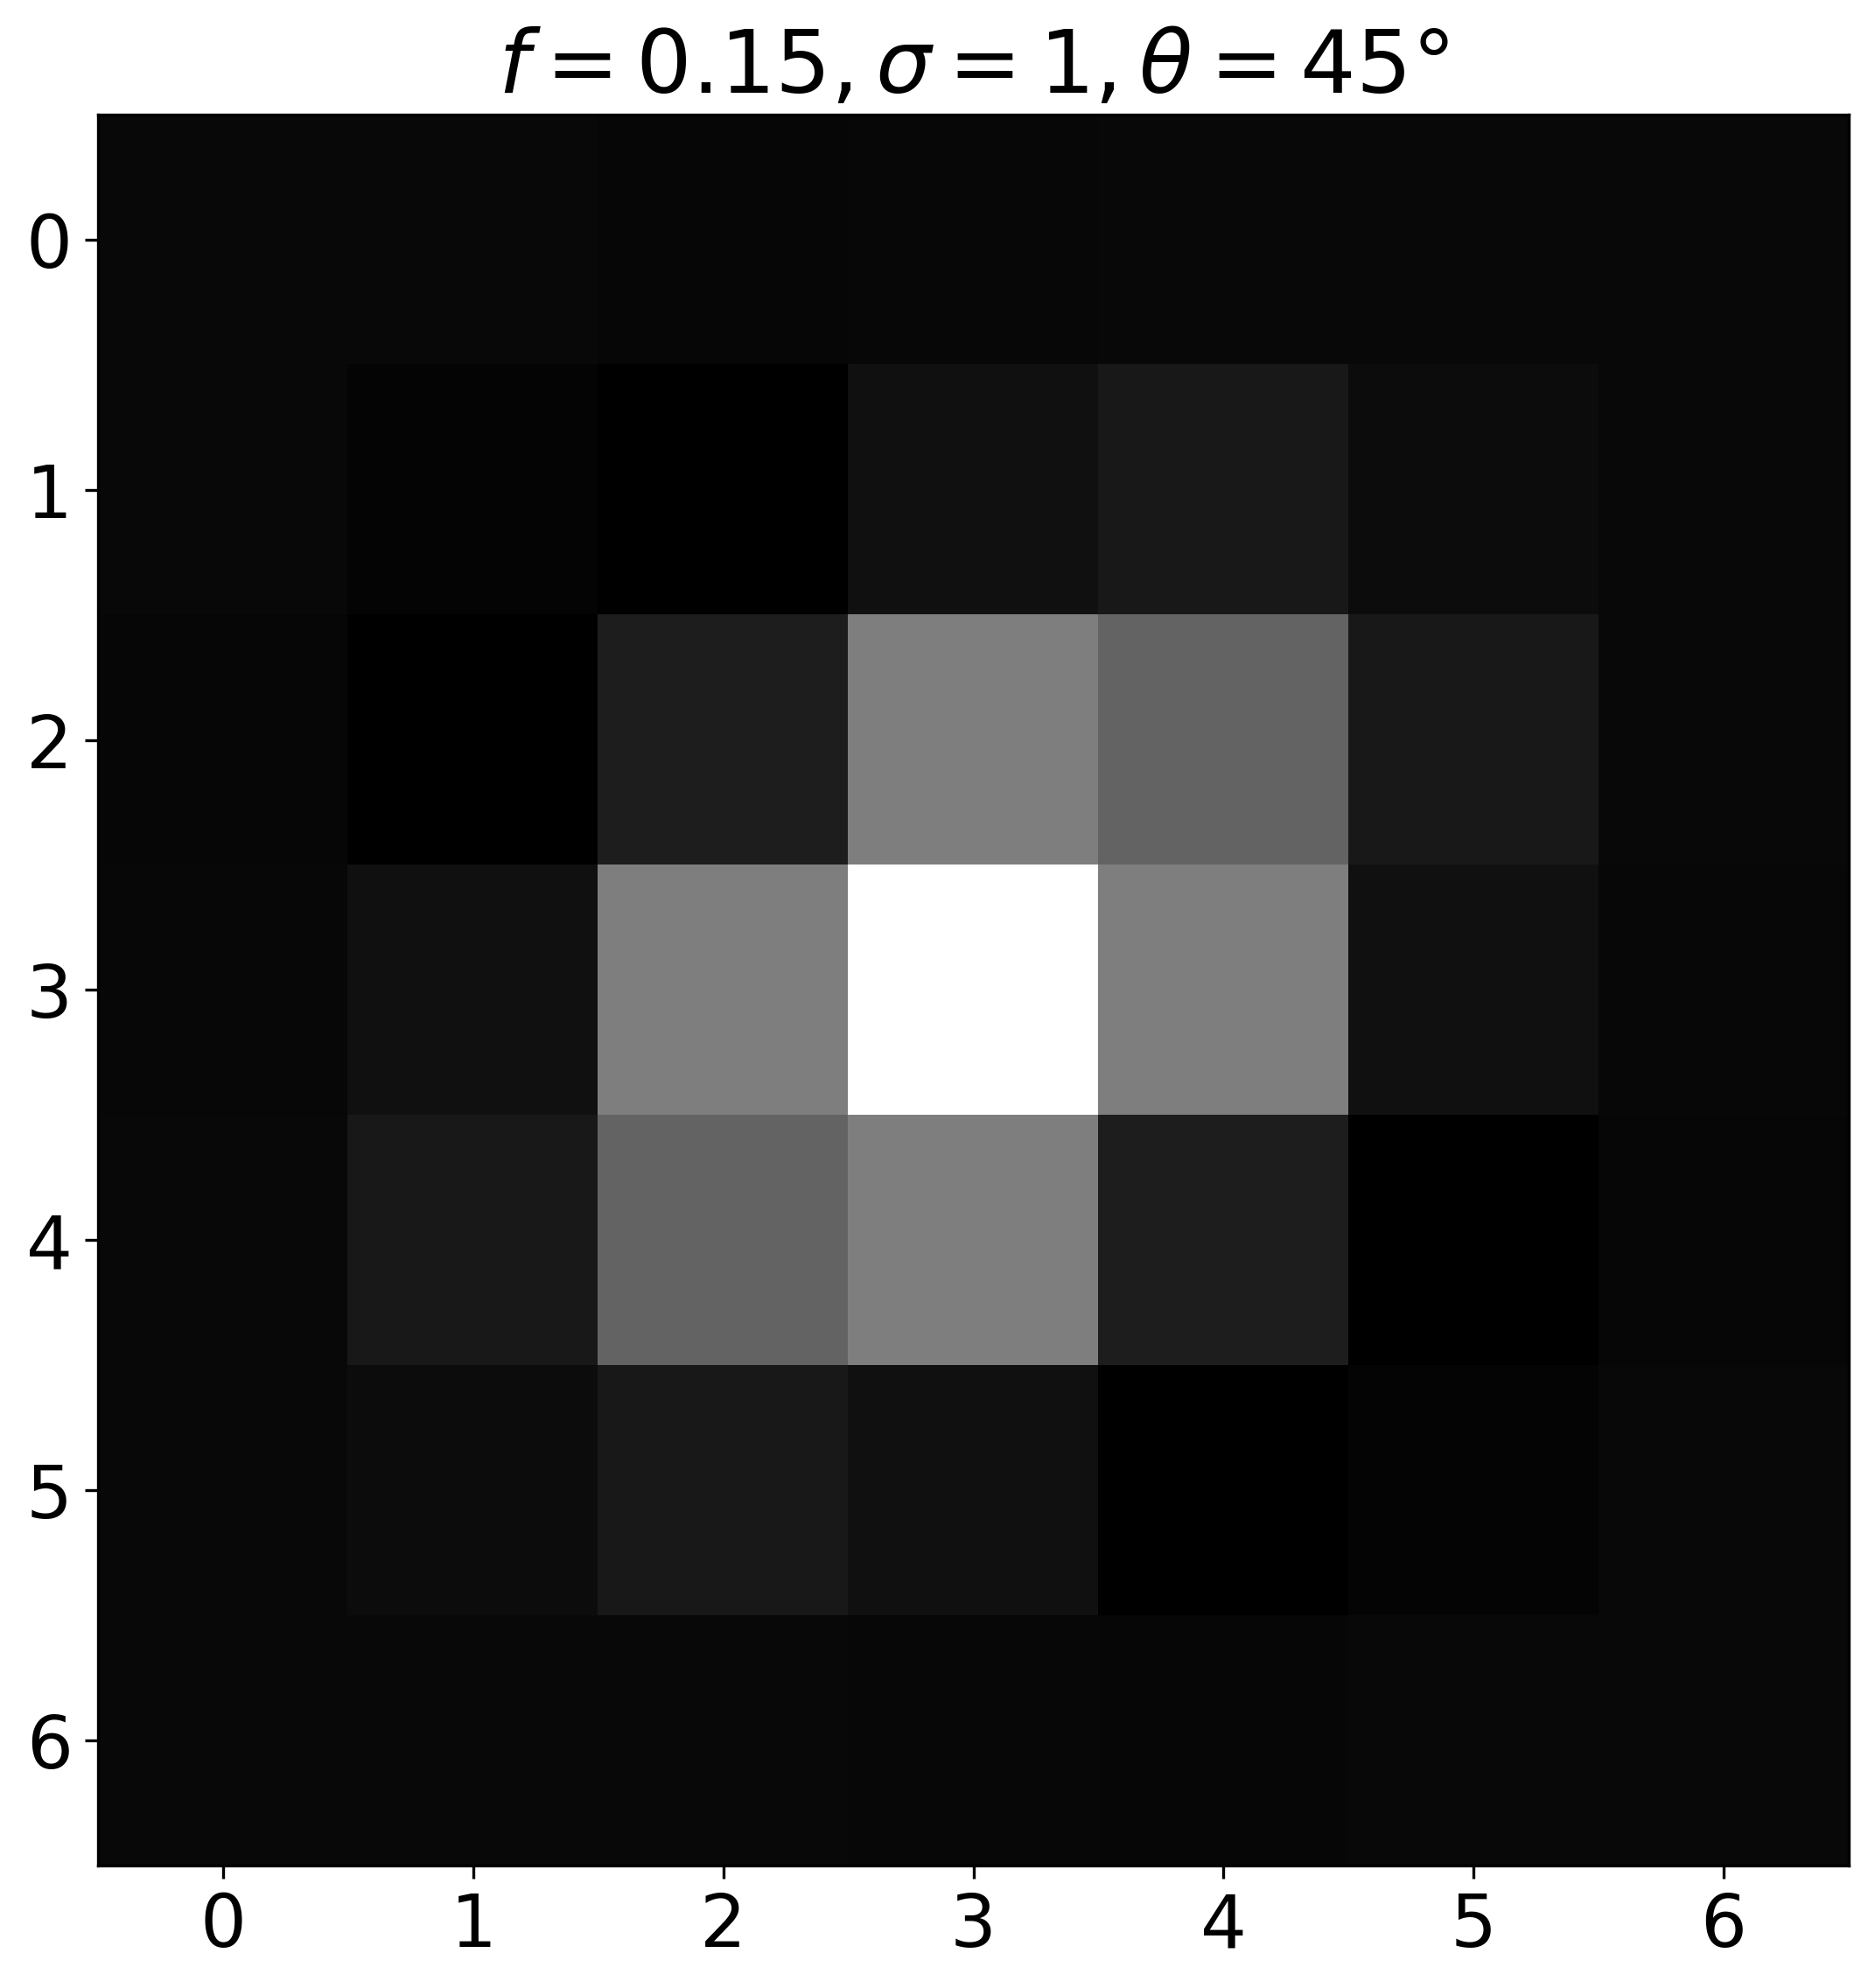
\includegraphics[width=\textwidth]{img/K3.png}
        \subcaption{Kernel 4}
      \end{subfigure}
      \begin{subfigure}[b]{0.3\textwidth}
        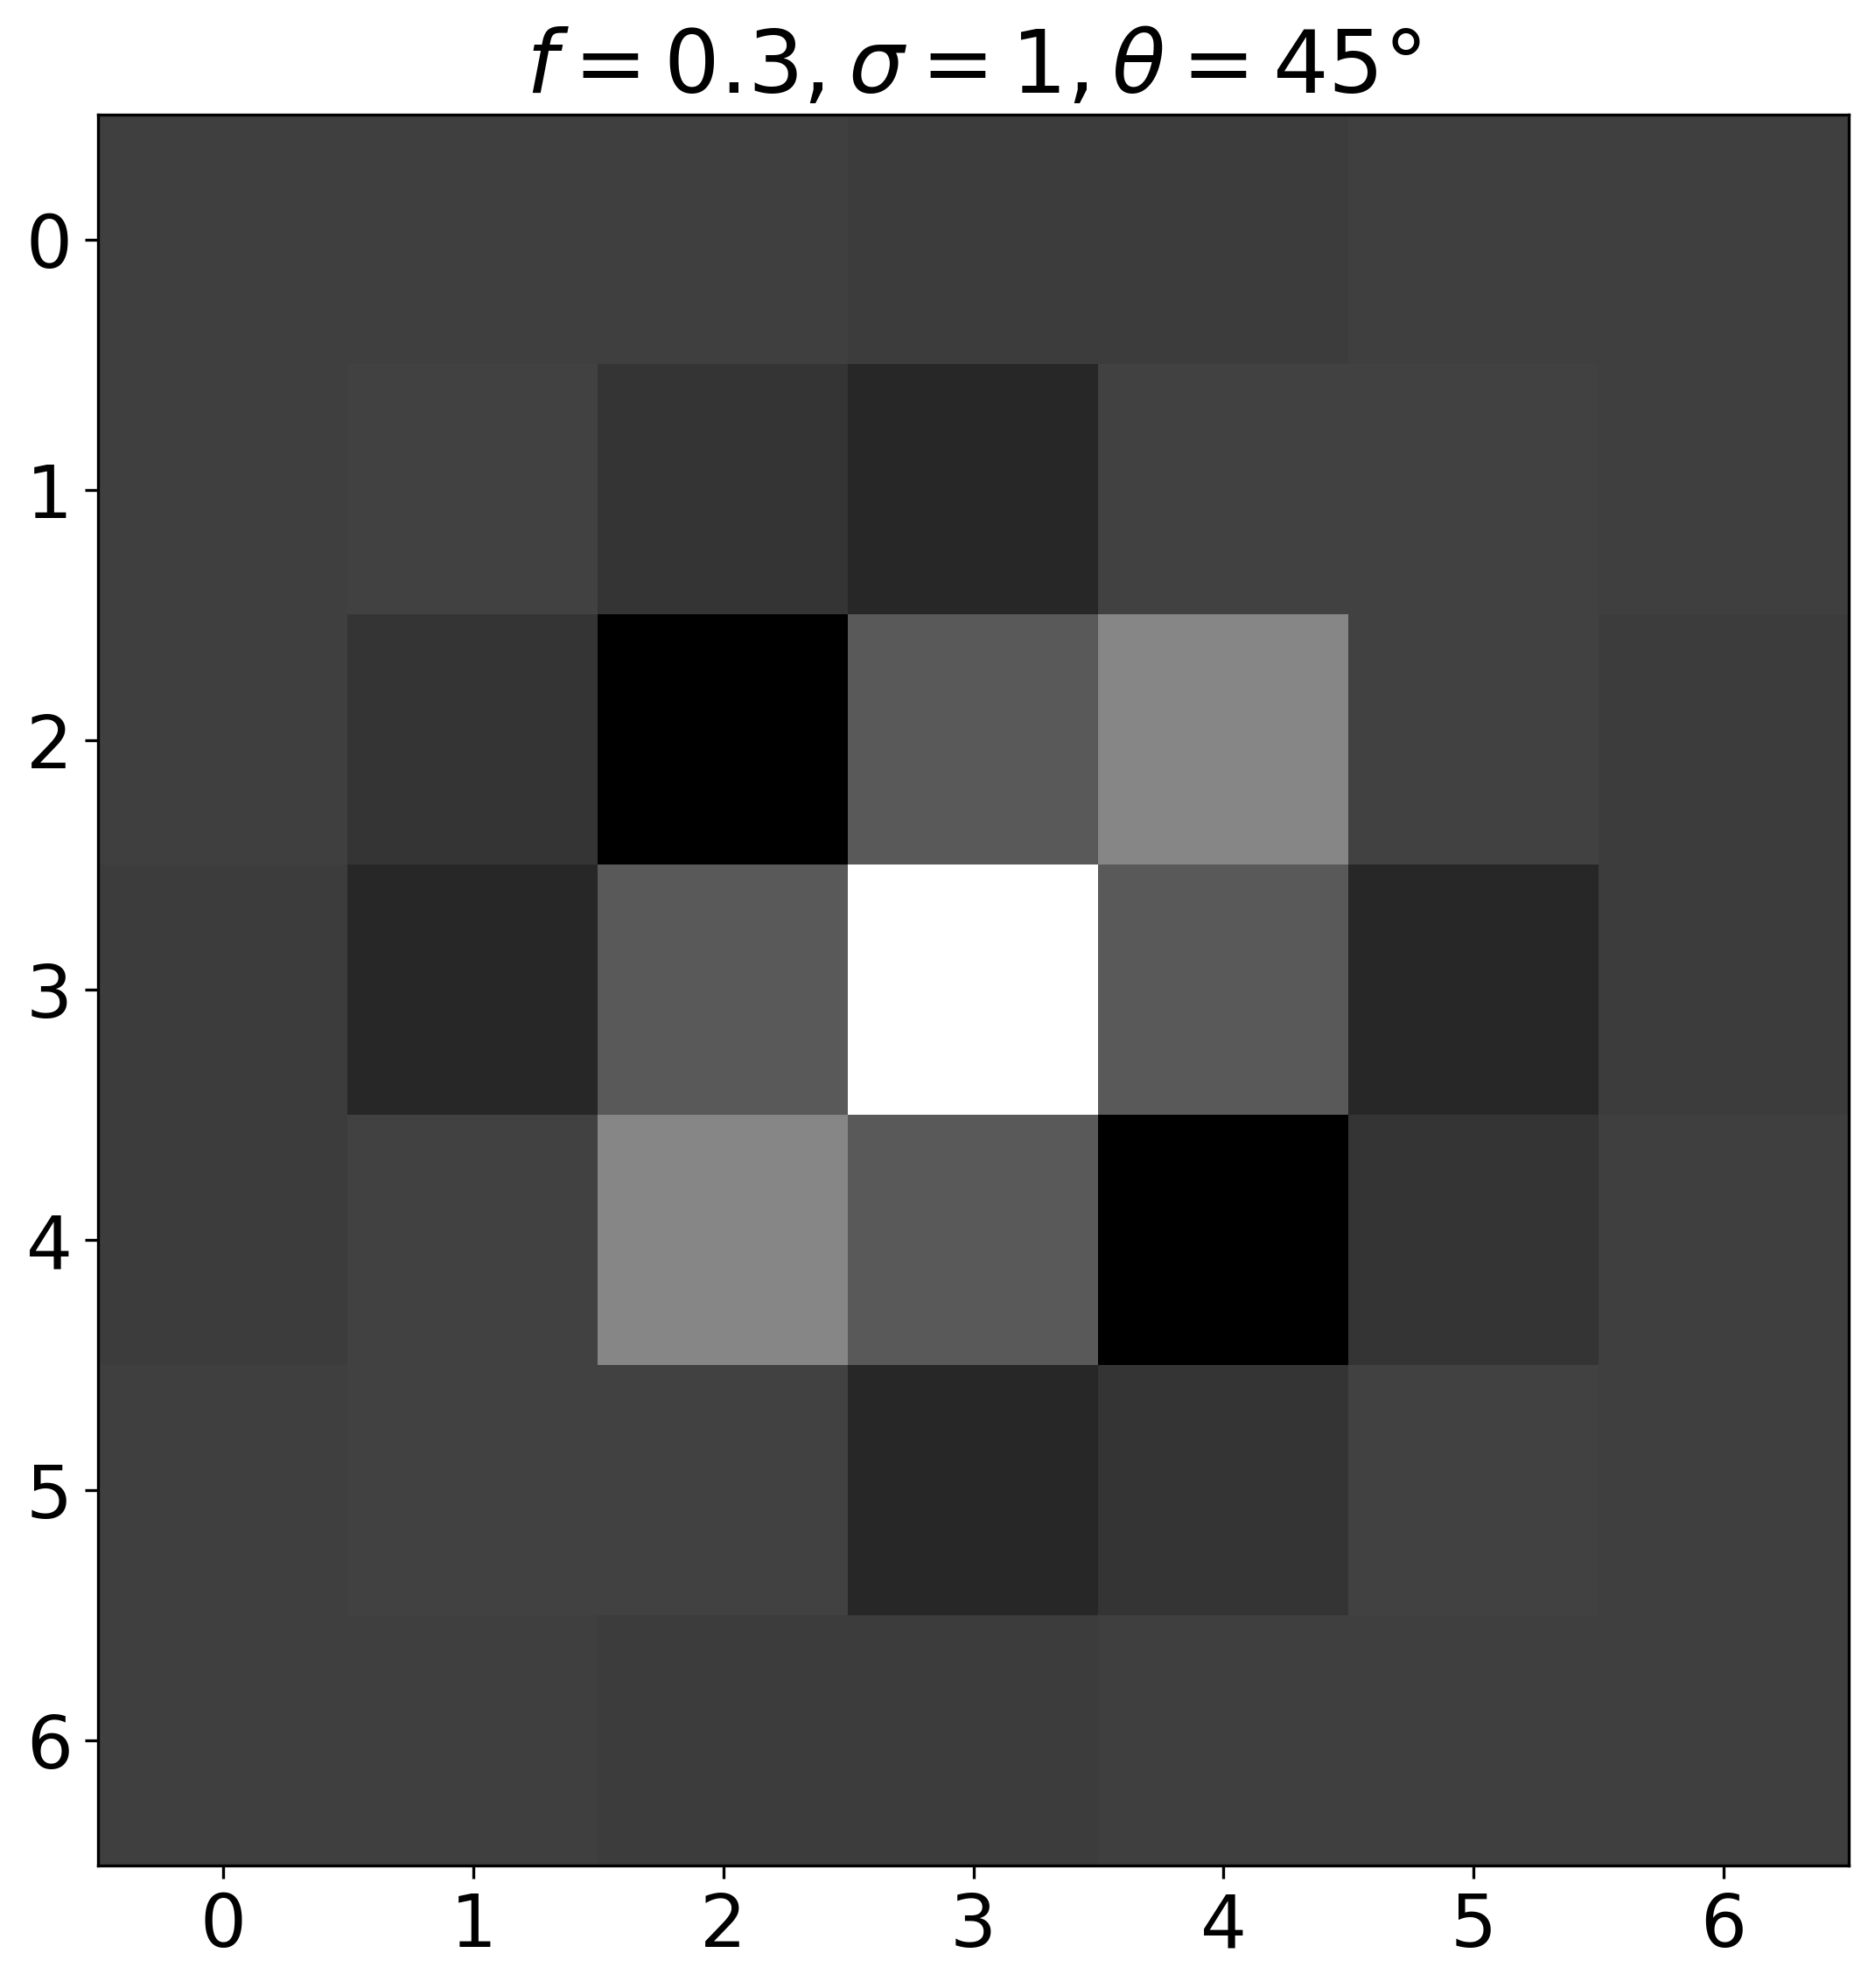
\includegraphics[width=\textwidth]{img/K4.png}
        \subcaption{Kernel 5}
      \end{subfigure}
      \begin{subfigure}[b]{0.3\textwidth}
        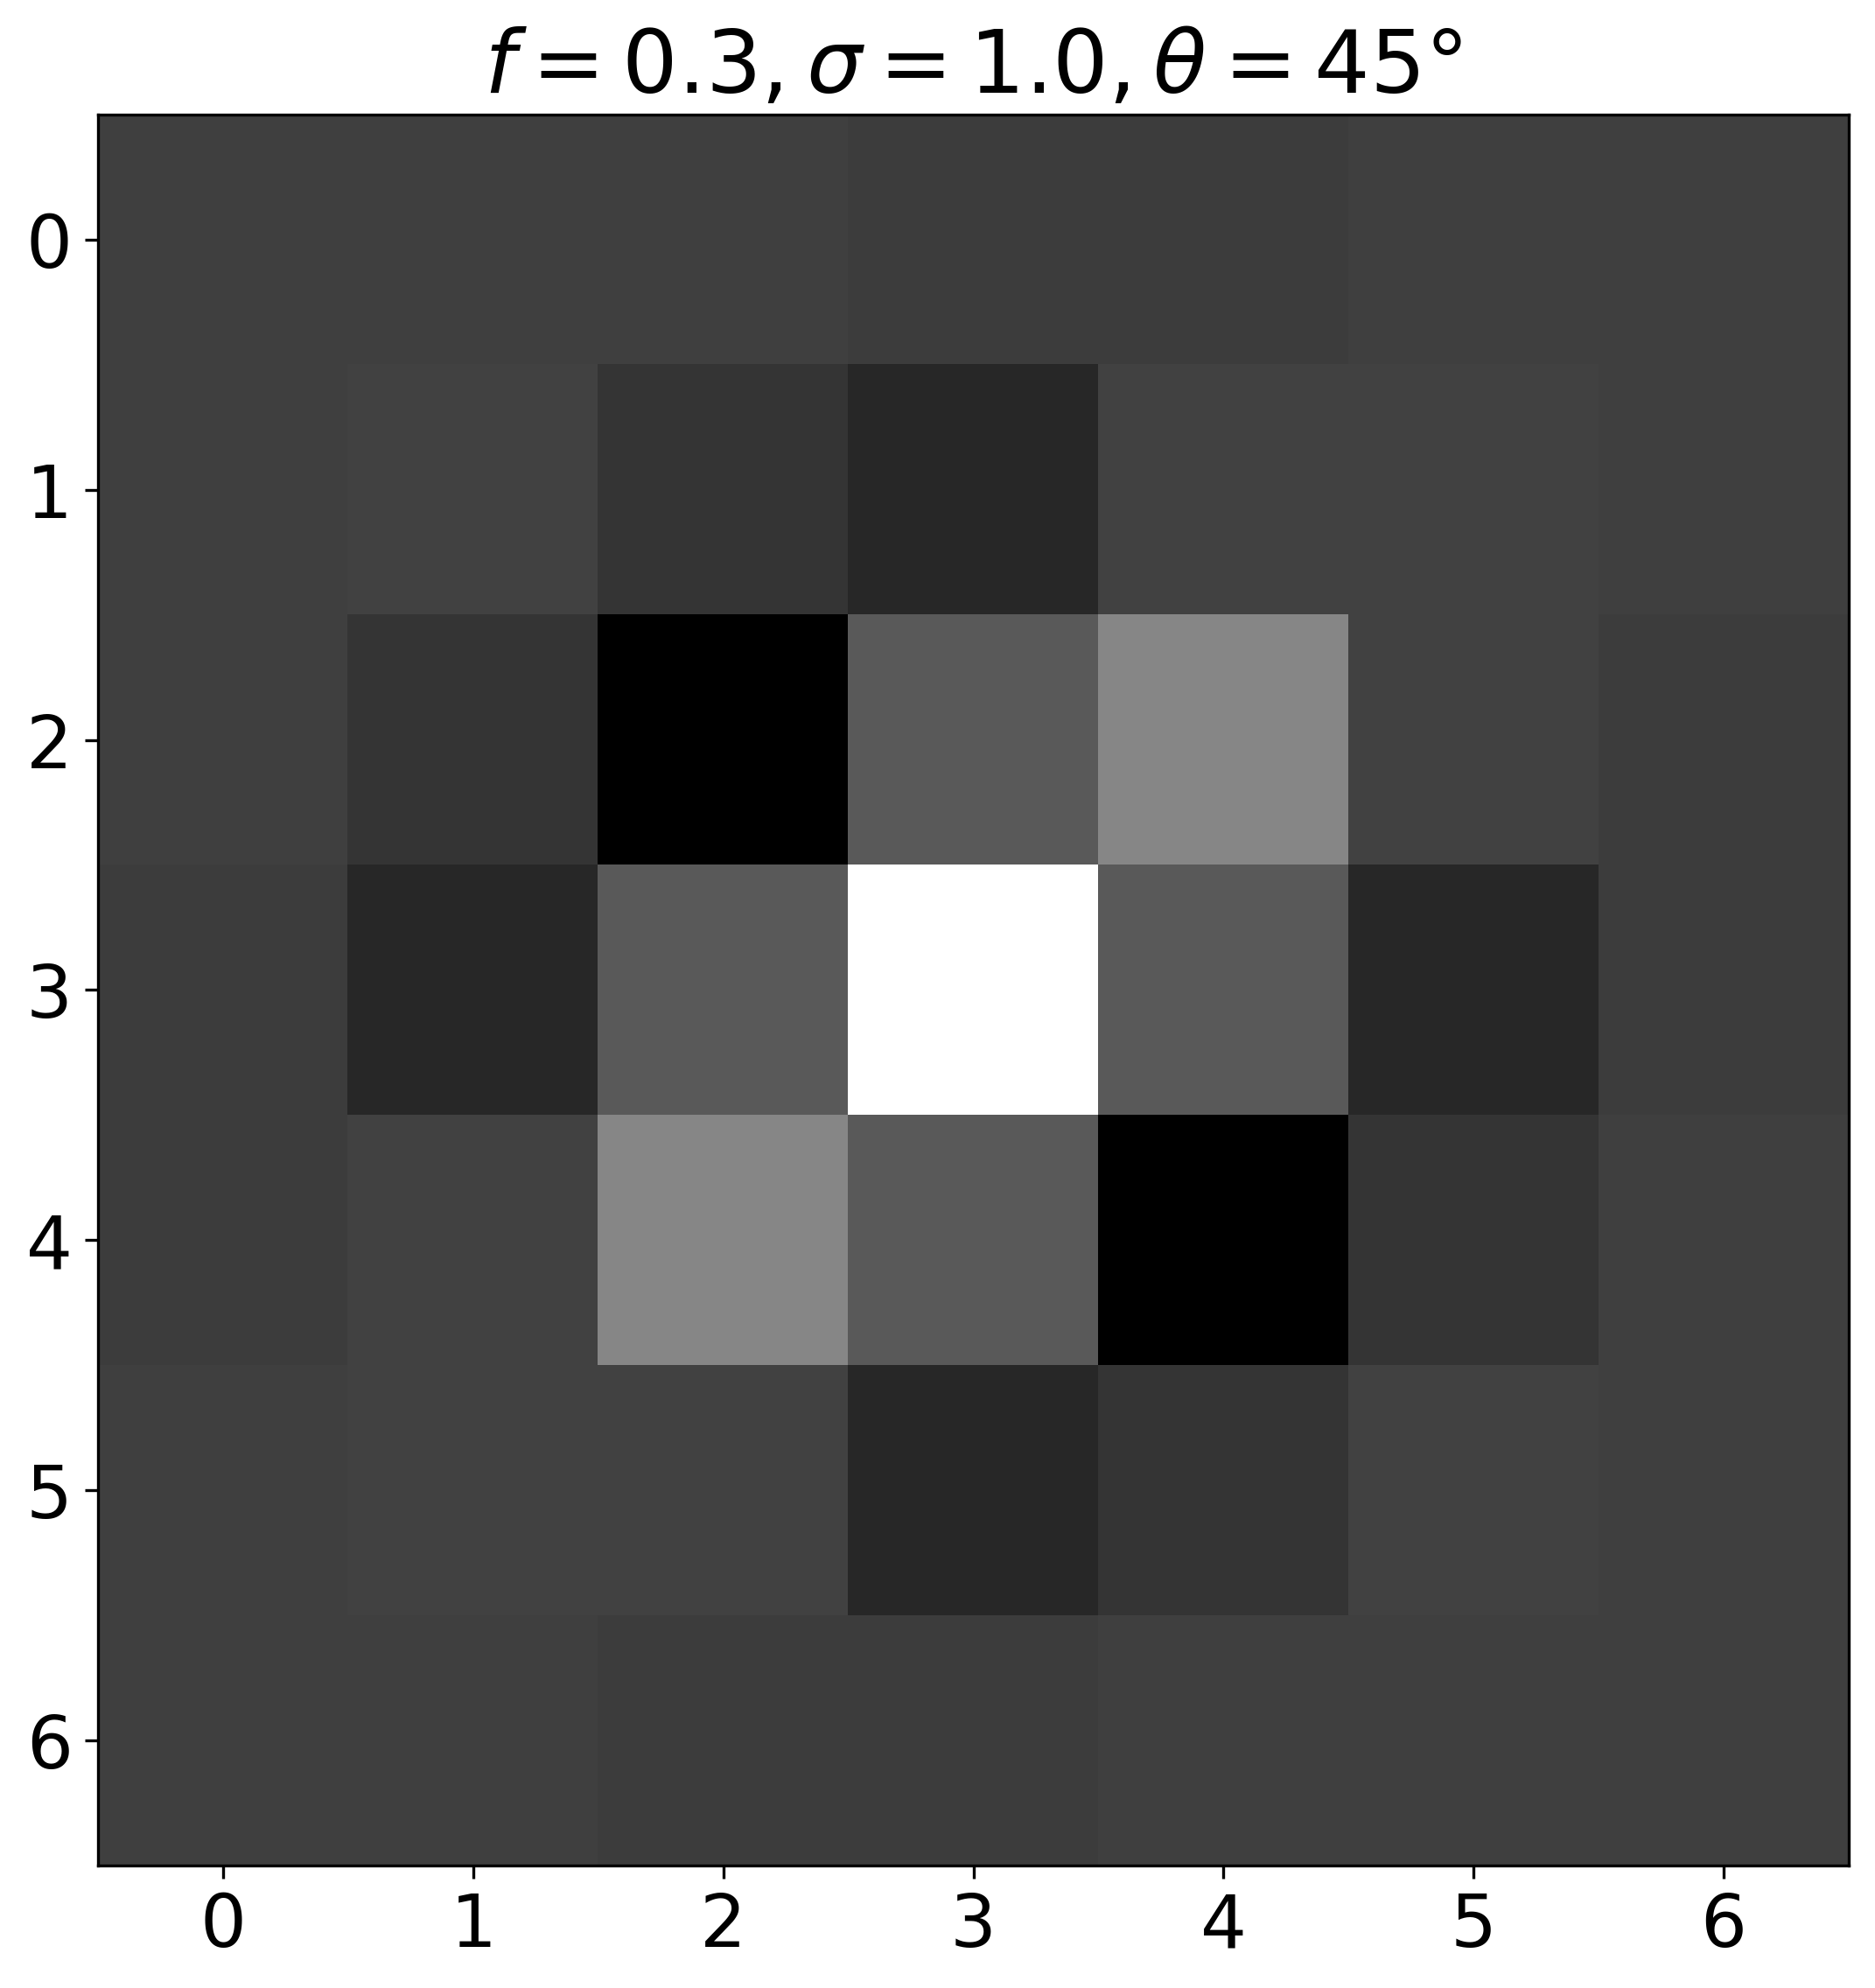
\includegraphics[width=\textwidth]{img/K5.png}
        \subcaption{Kernel 6}
      \end{subfigure}

      \begin{subfigure}[b]{0.3\textwidth}
        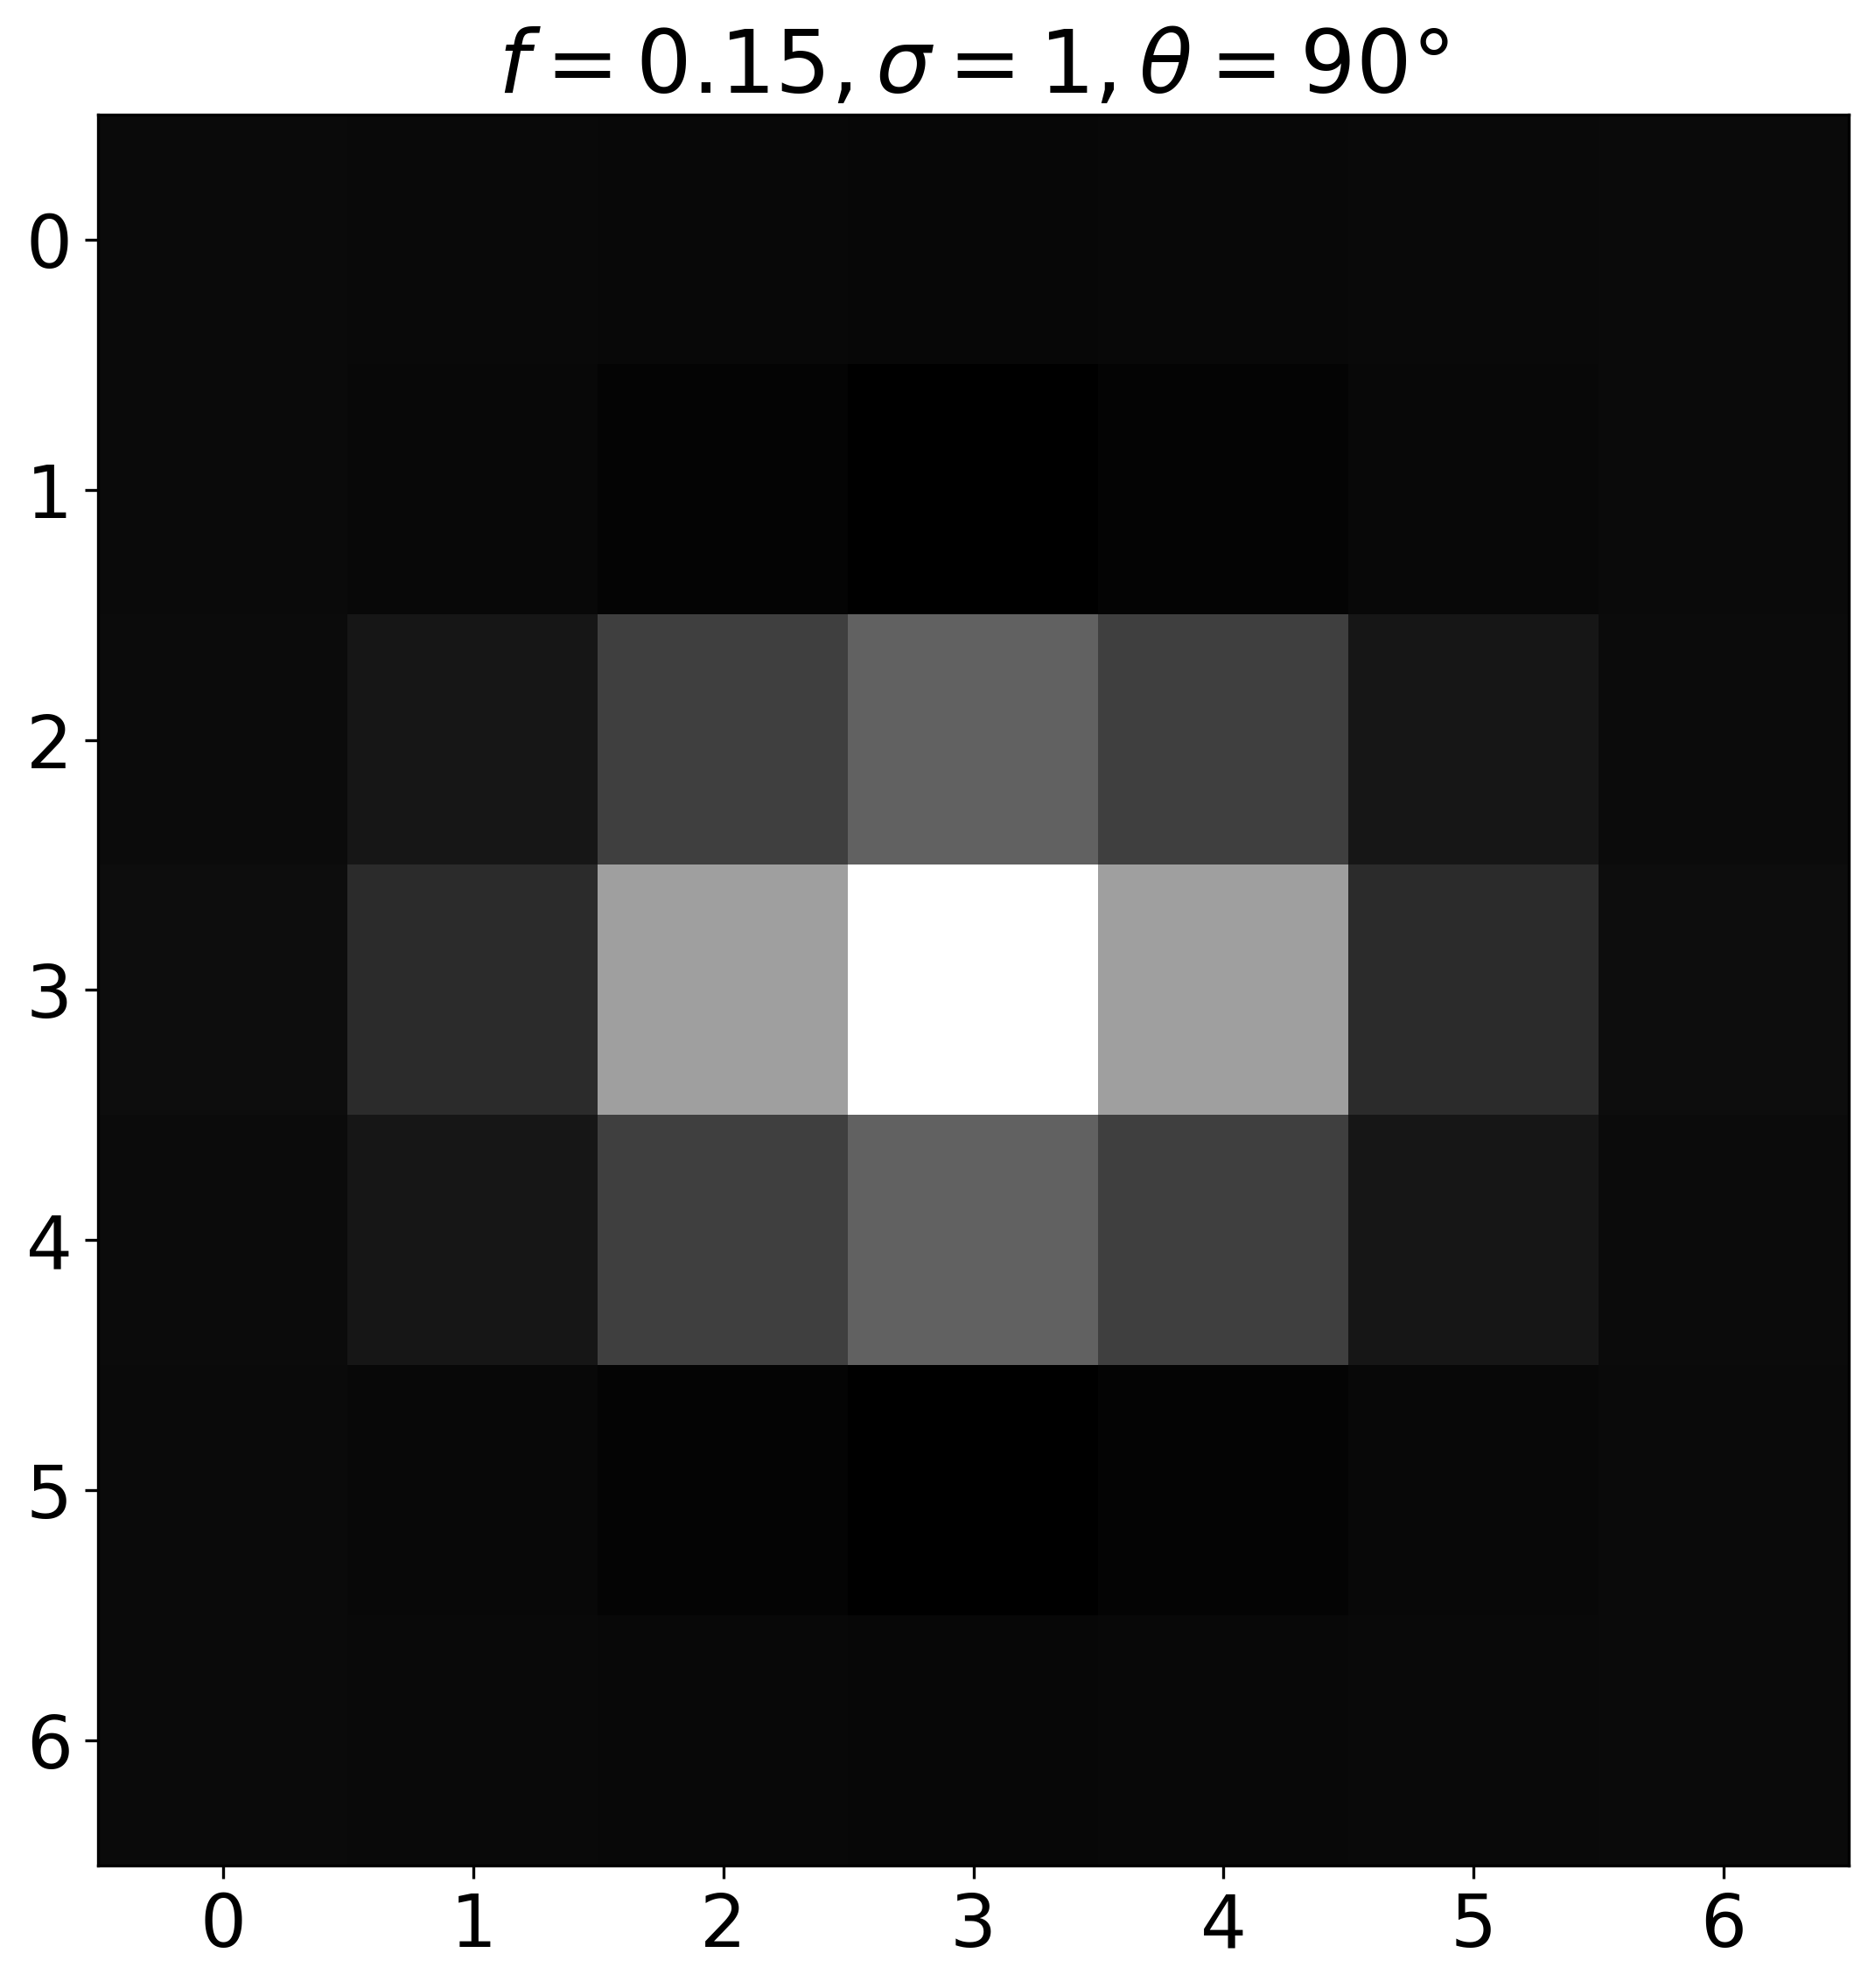
\includegraphics[width=\textwidth]{img/K6.png}
        \subcaption{Kernel 7}
      \end{subfigure}
      \begin{subfigure}[b]{0.3\textwidth}
        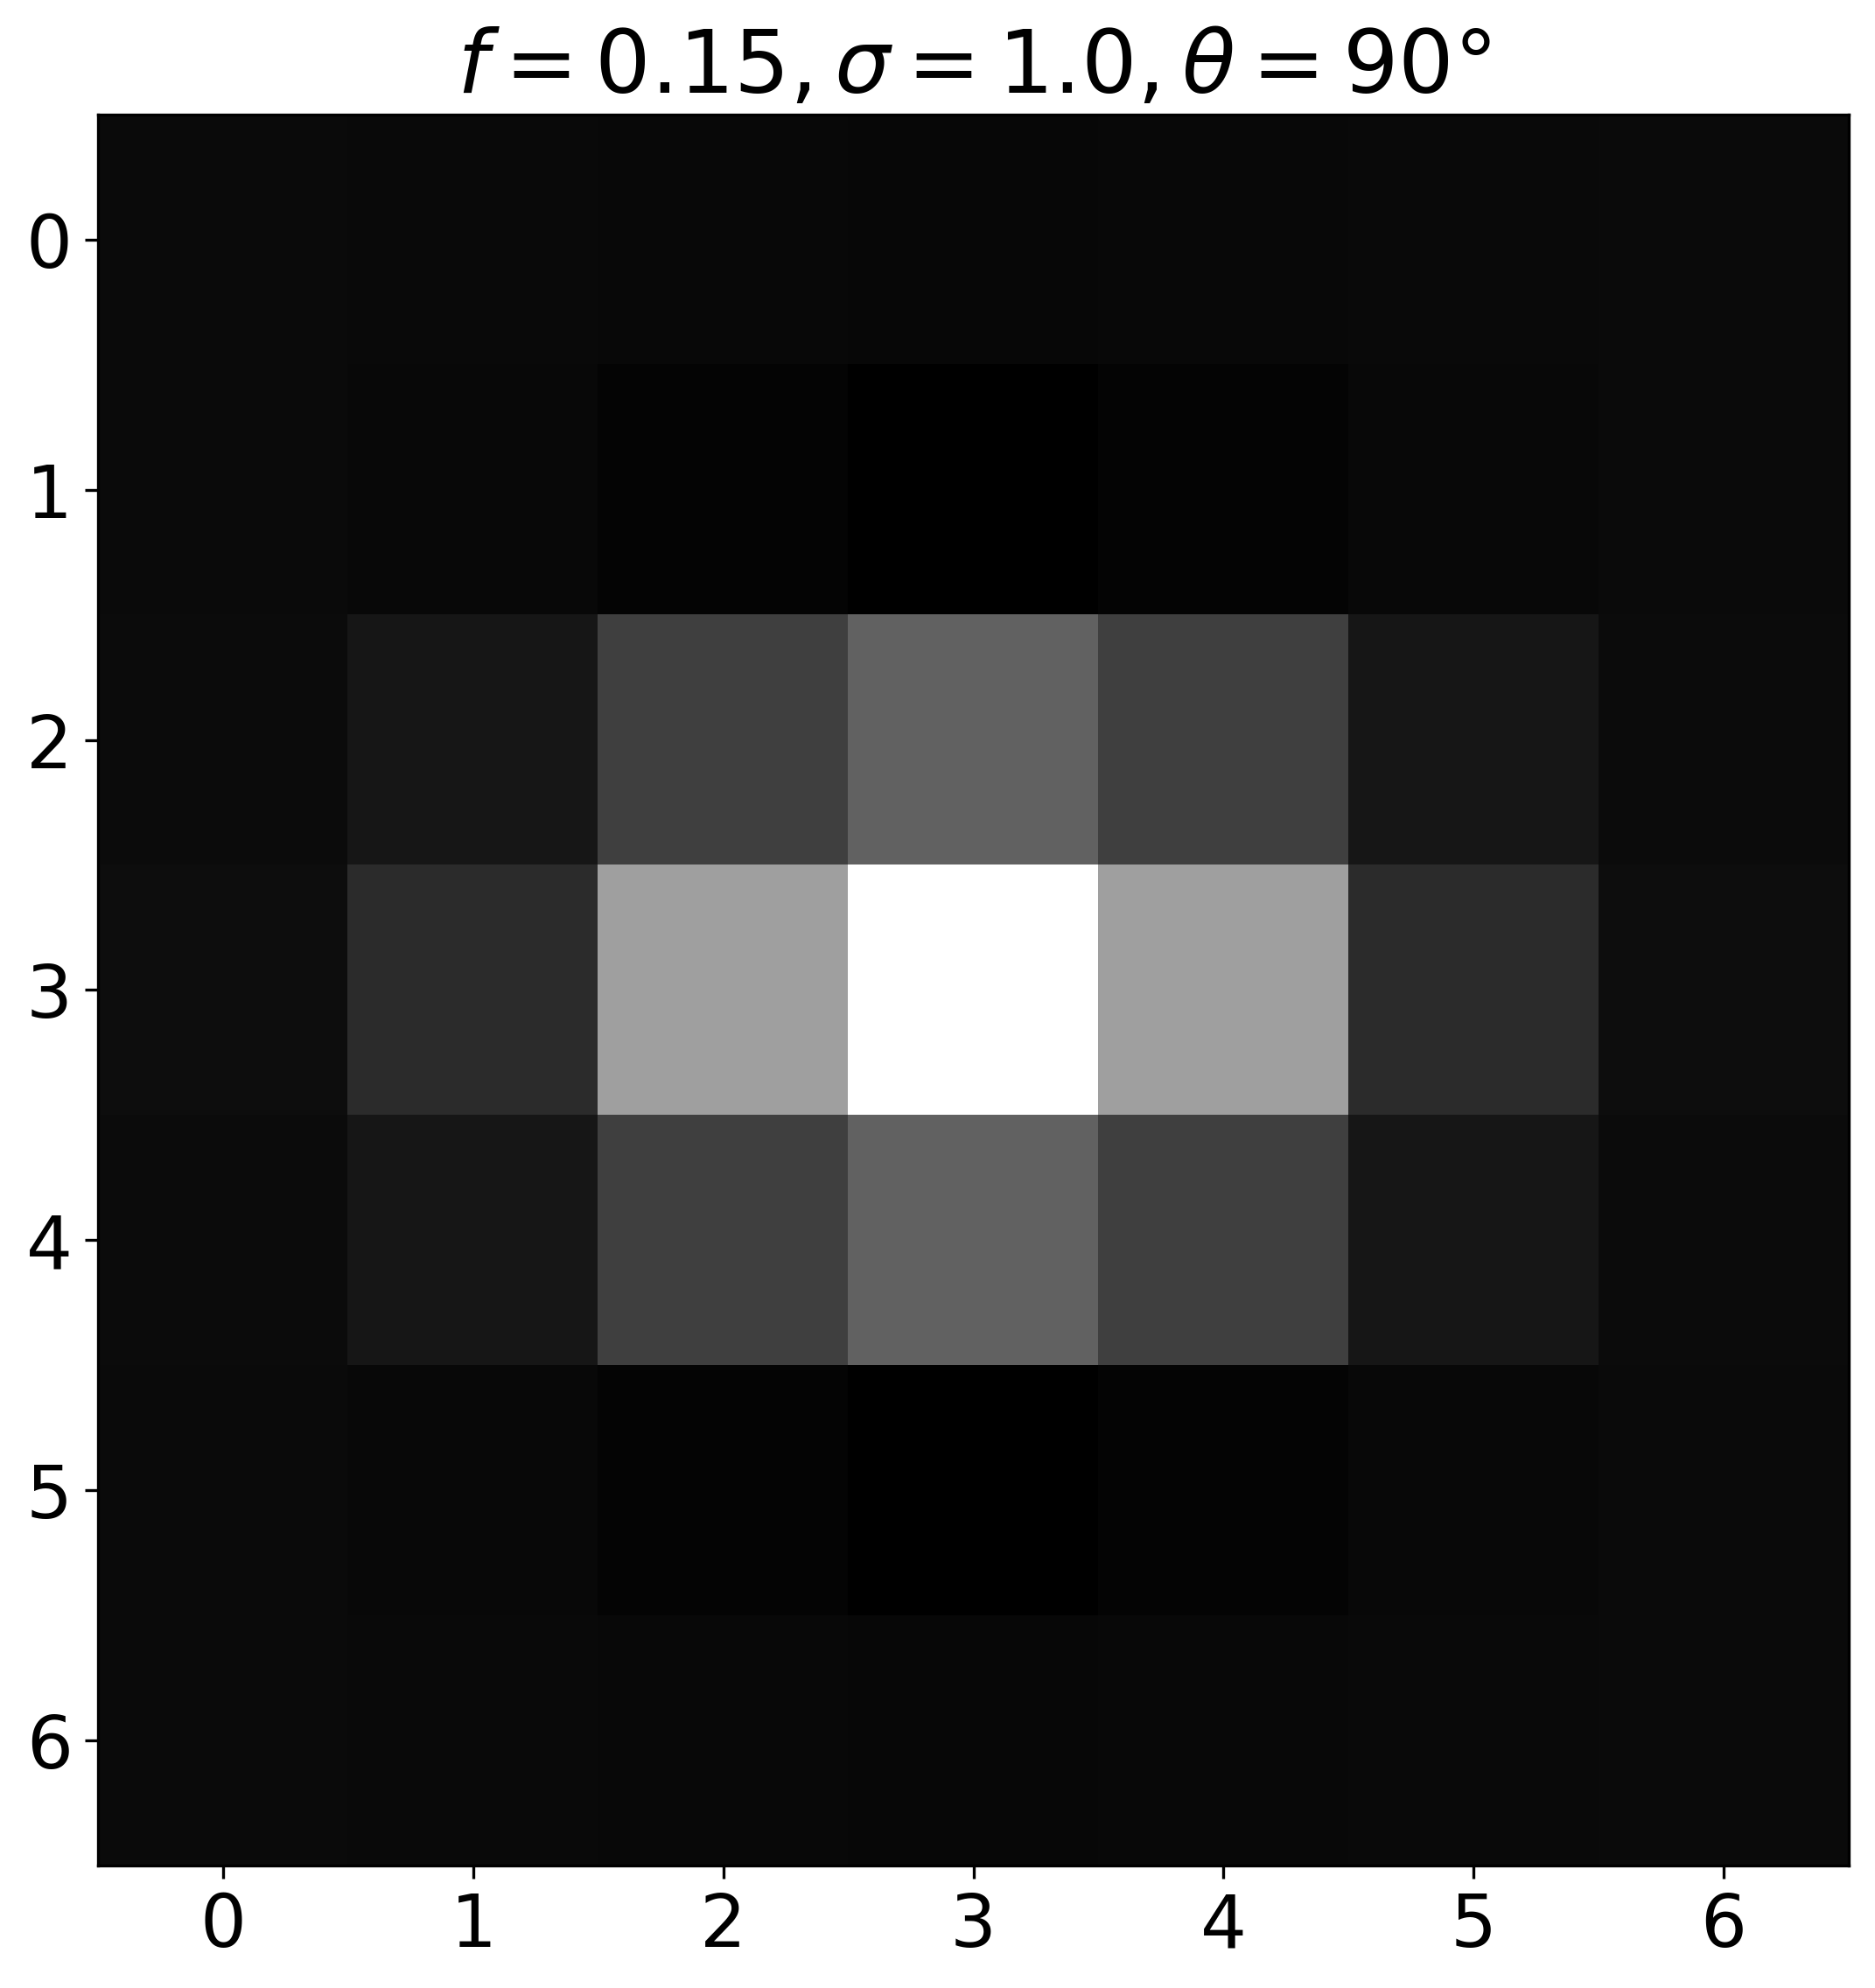
\includegraphics[width=\textwidth]{img/K7.png}
        \subcaption{Kernel 8}
      \end{subfigure}
      \begin{subfigure}[b]{0.3\textwidth}
        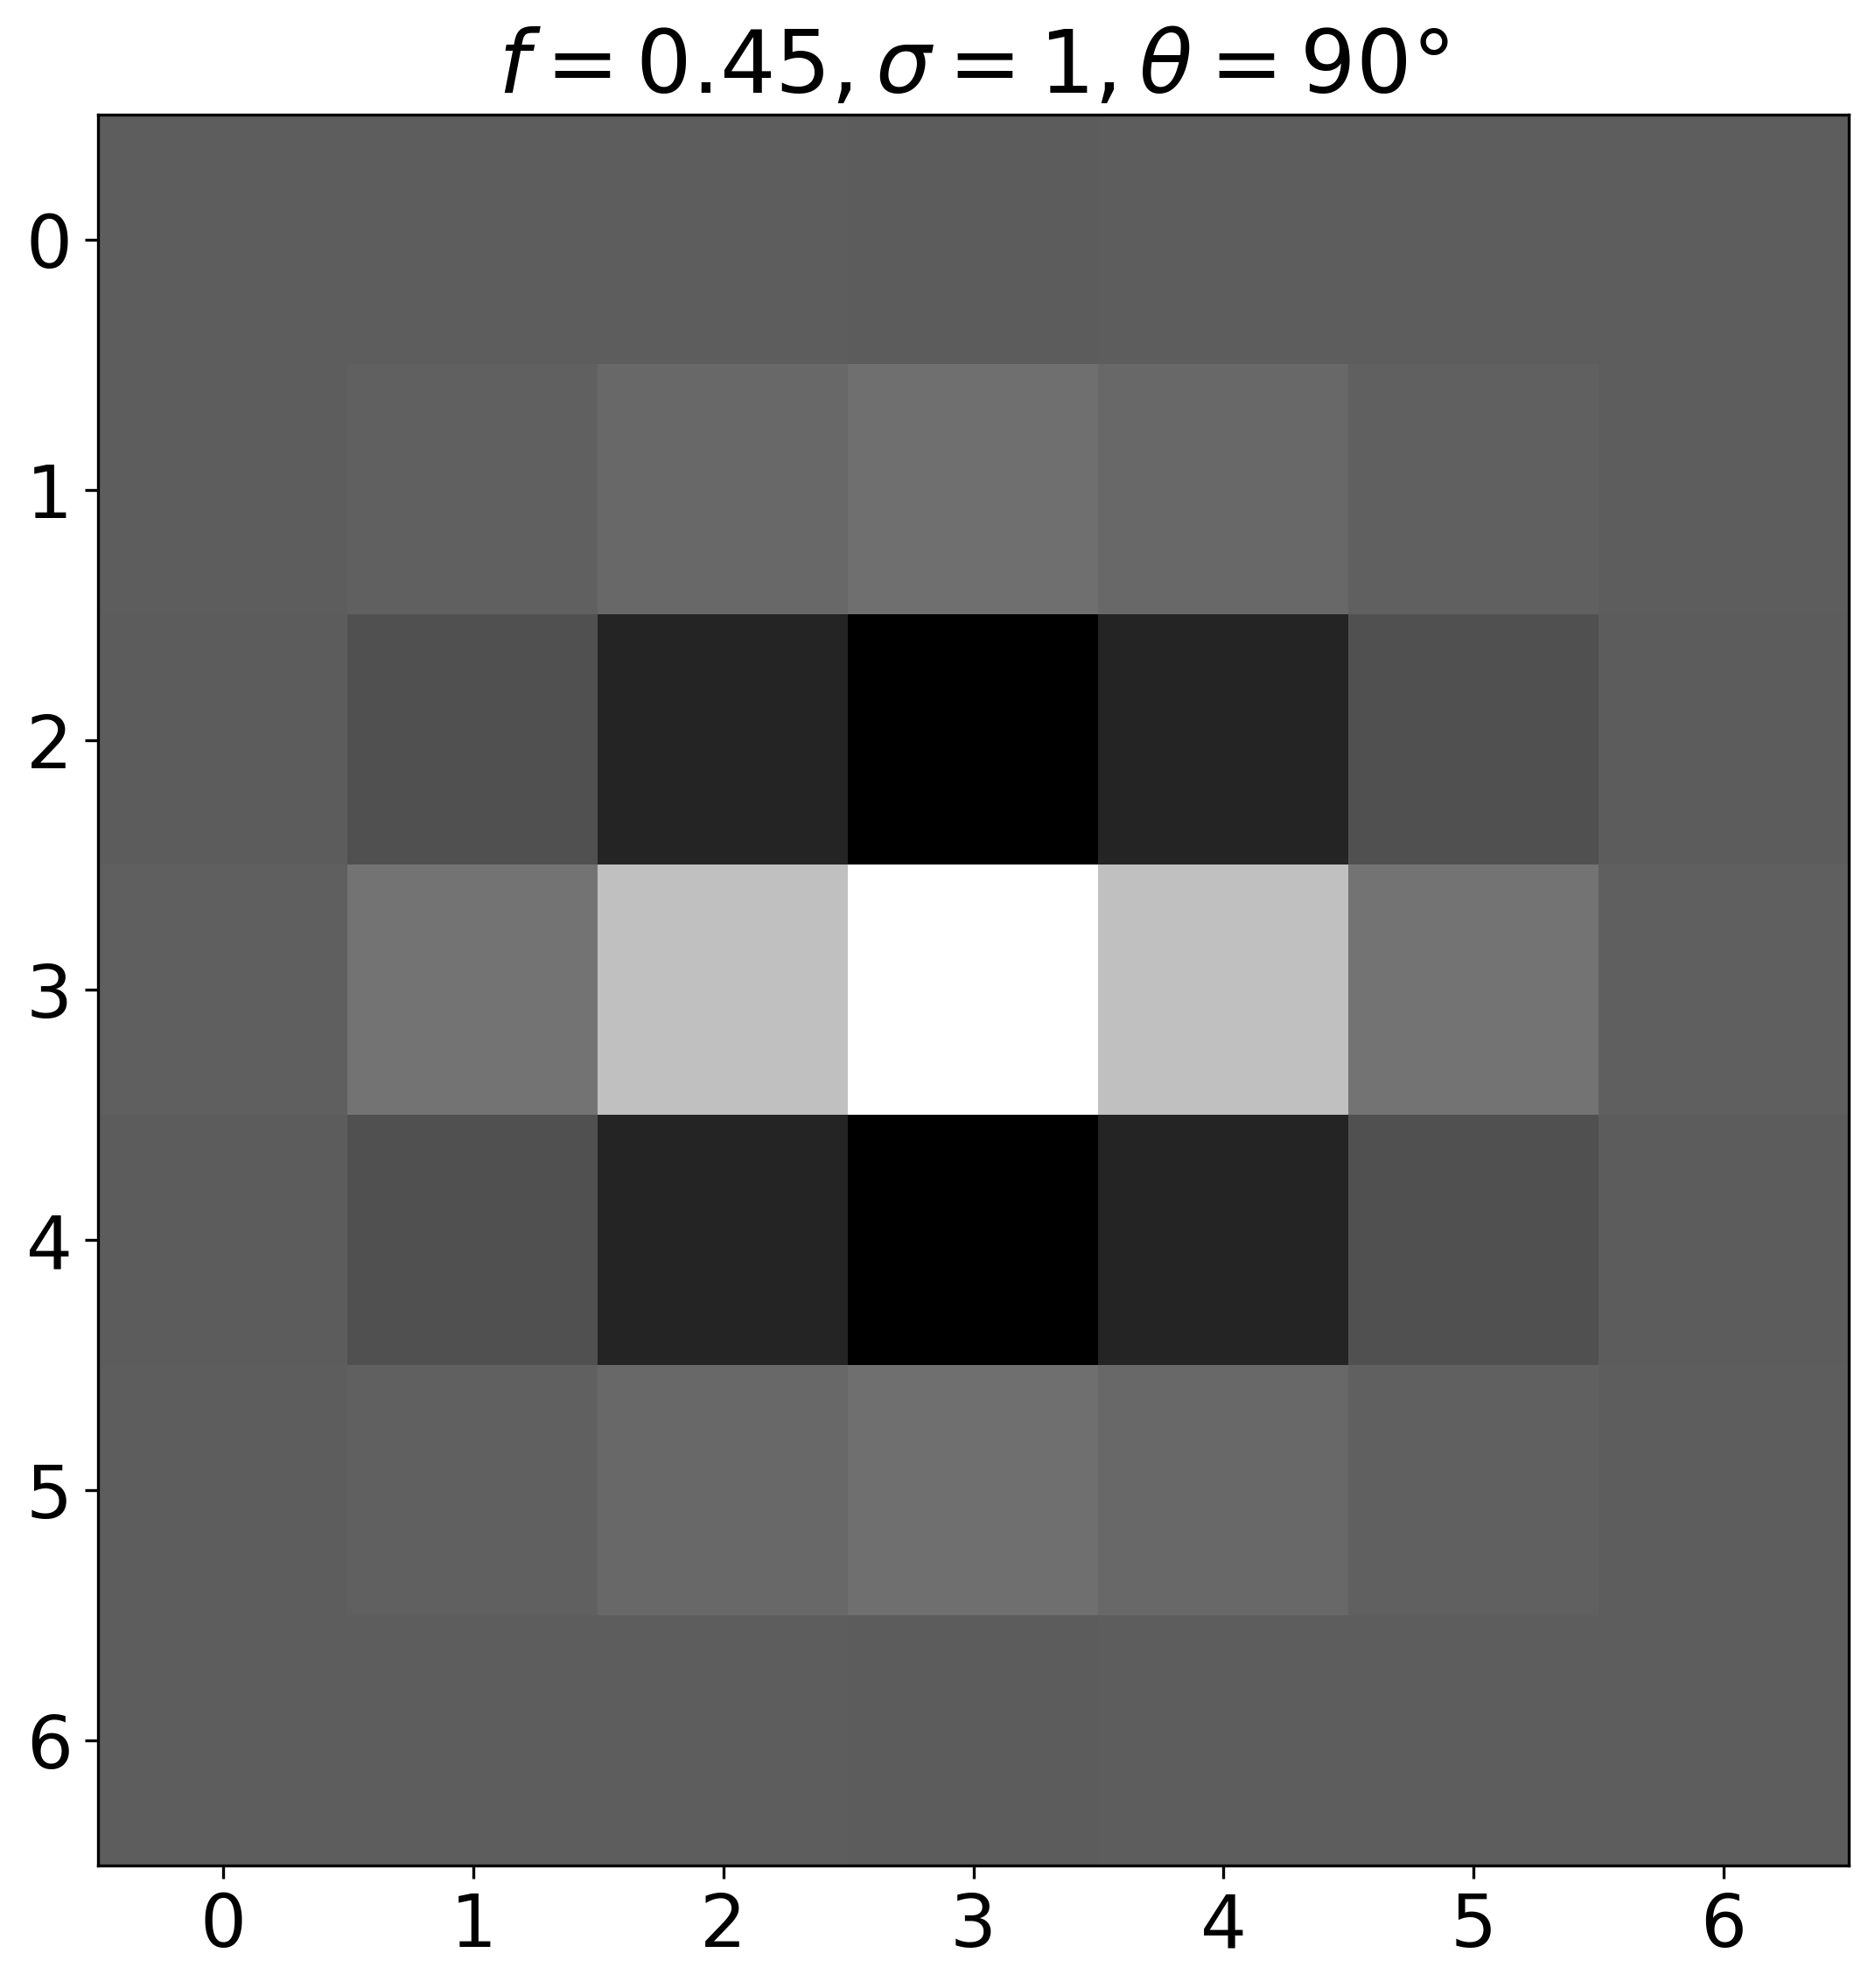
\includegraphics[width=\textwidth]{img/K8.png}
        \subcaption{Kernel 9}
      \end{subfigure}

      \begin{subfigure}[b]{0.3\textwidth}
        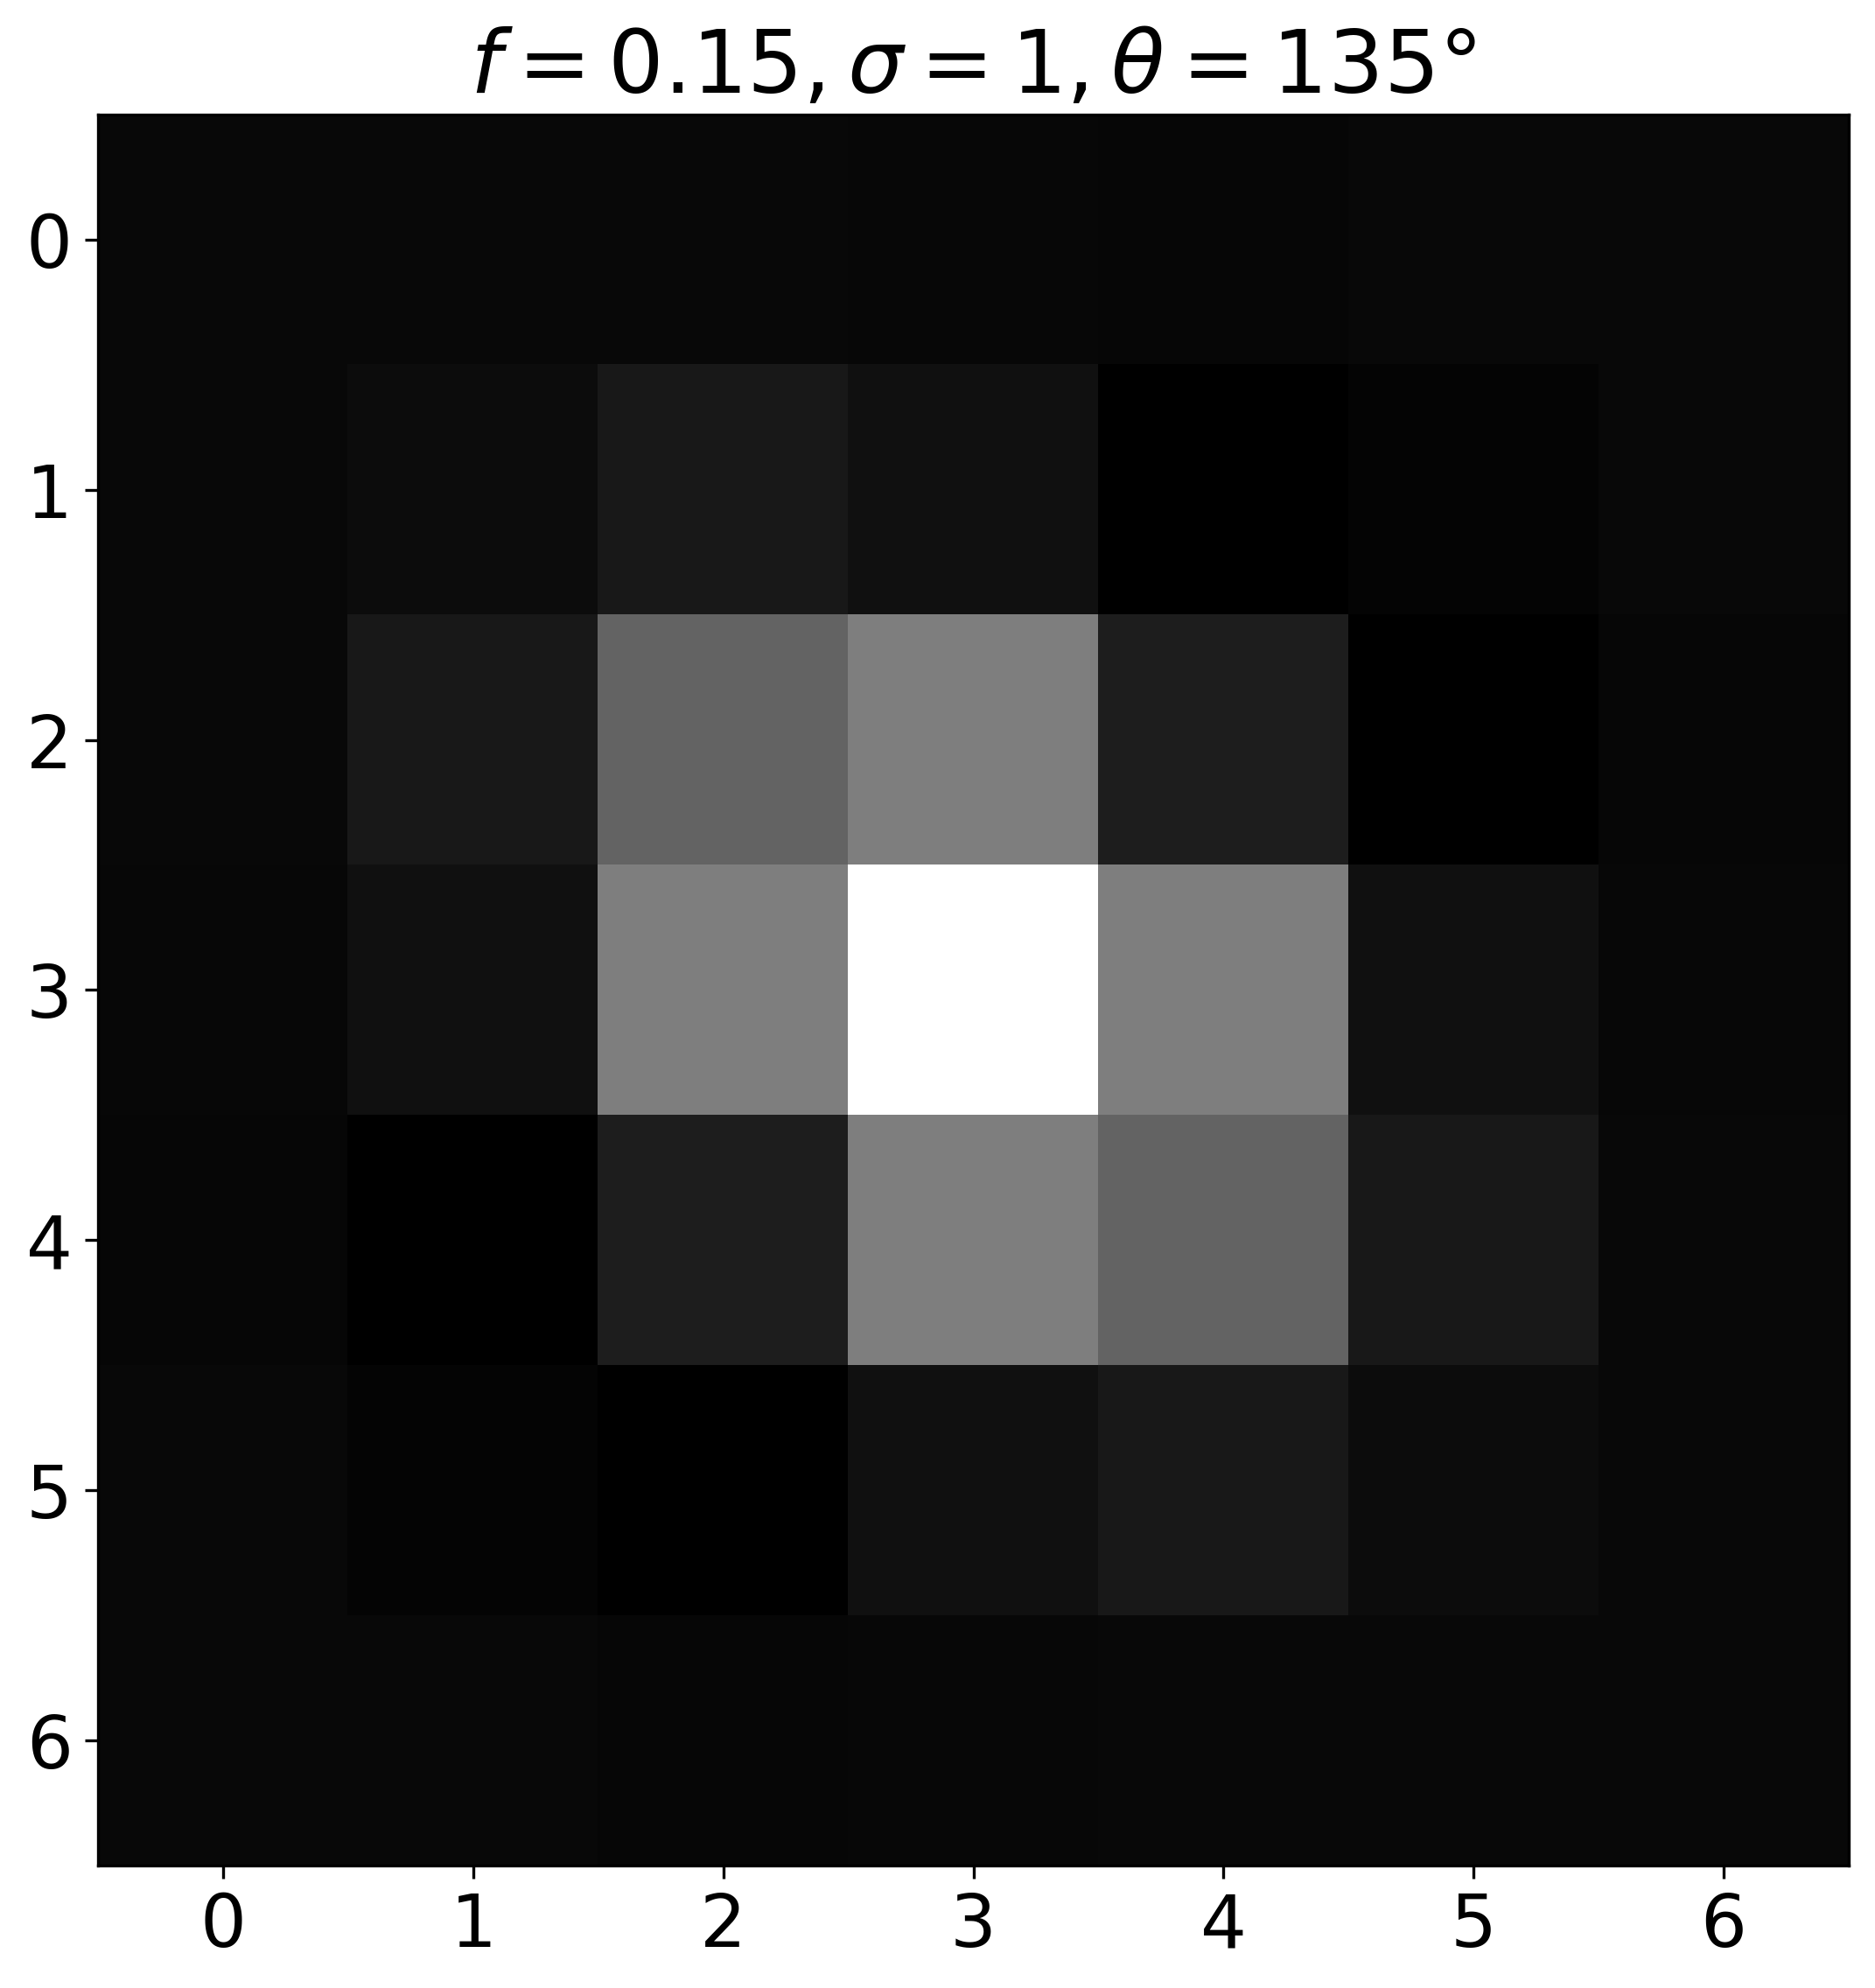
\includegraphics[width=\textwidth]{img/K9.png}
        \subcaption{Kernel 10}
      \end{subfigure}
      \begin{subfigure}[b]{0.3\textwidth}
        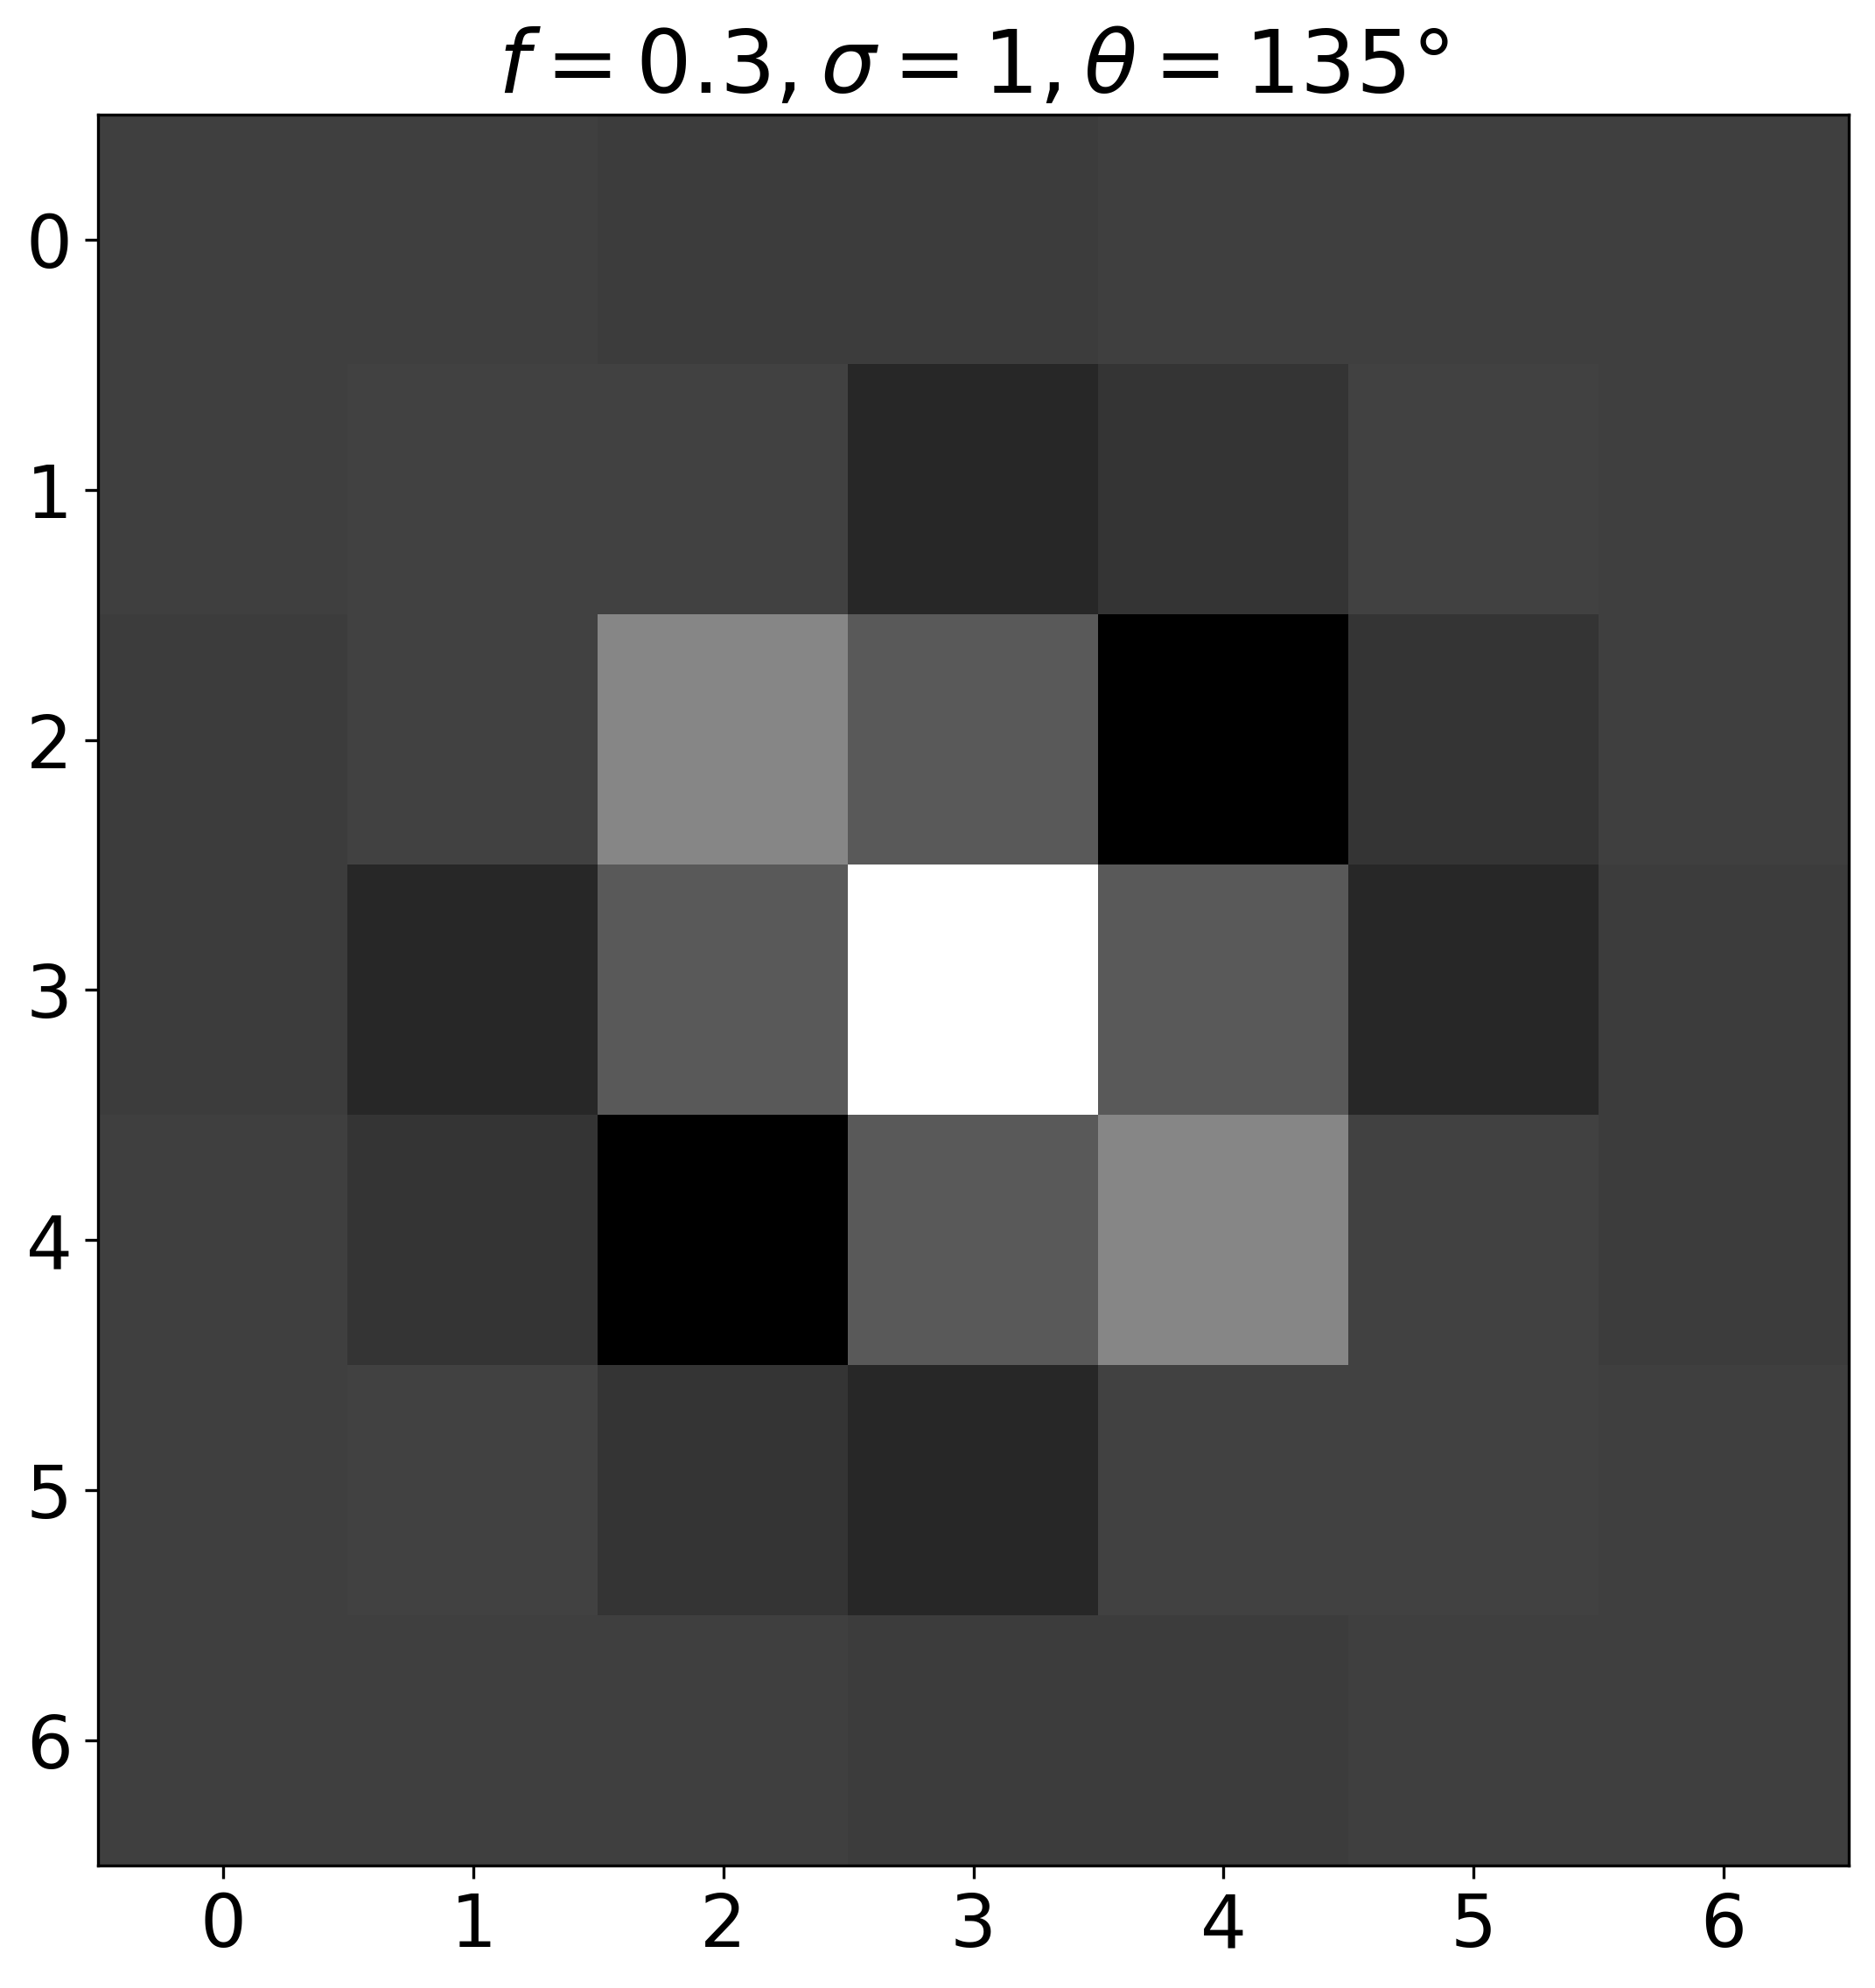
\includegraphics[width=\textwidth]{img/K10.png}
        \subcaption{Kernel 11}
      \end{subfigure}
      \begin{subfigure}[b]{0.3\textwidth}
        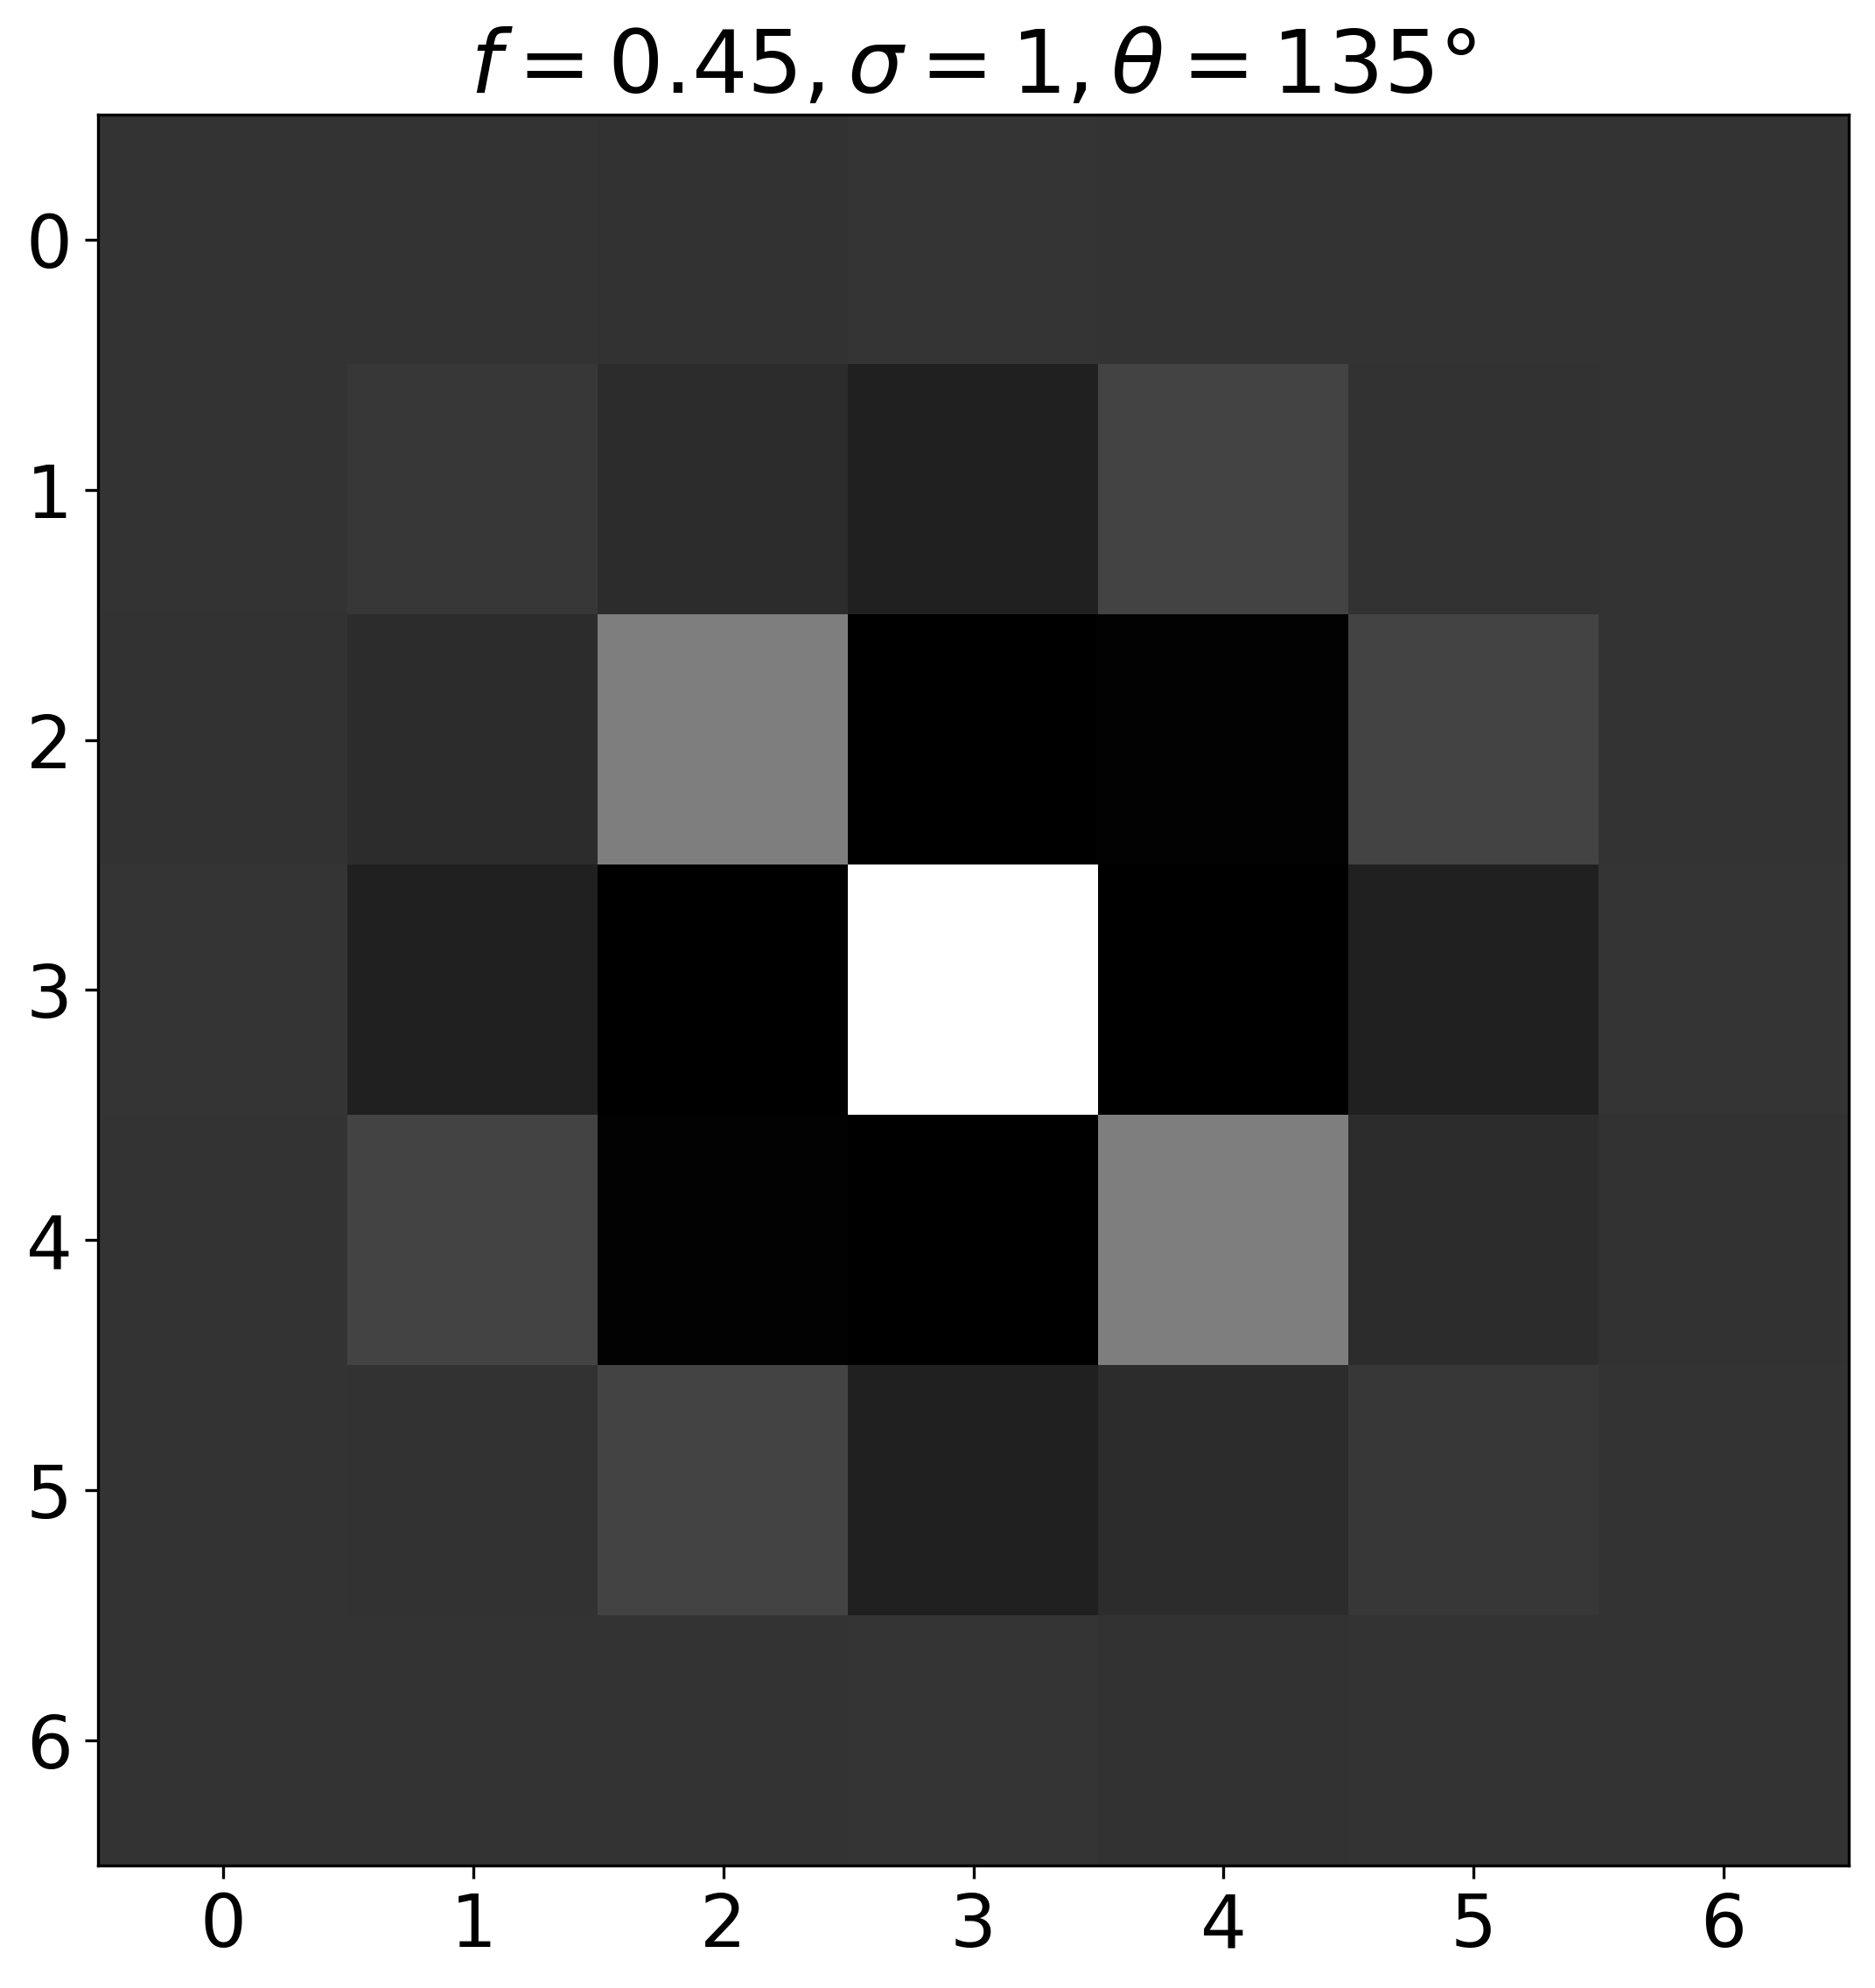
\includegraphics[width=\textwidth]{img/K11.png}
        \subcaption{Kernel 12}
      \end{subfigure}
      \caption{Filter bank of 12 gabor filters with 4 rotations and a $\sigma=1\ $ and $\ f = 0.15, 0,35 \text{ and } 0.4$\label{fig:gaborbank}}%
    \end{figure}
%  
    \noindent
    The kernels mainly act as a edge and structure detection algorithm in this case as shown in \cref{fig:gaborresults}, that shows extracted features of some example bands.
  \begin{figure}[!htbp]
      \centering
      \begin{subfigure}[b]{0.3\textwidth}
        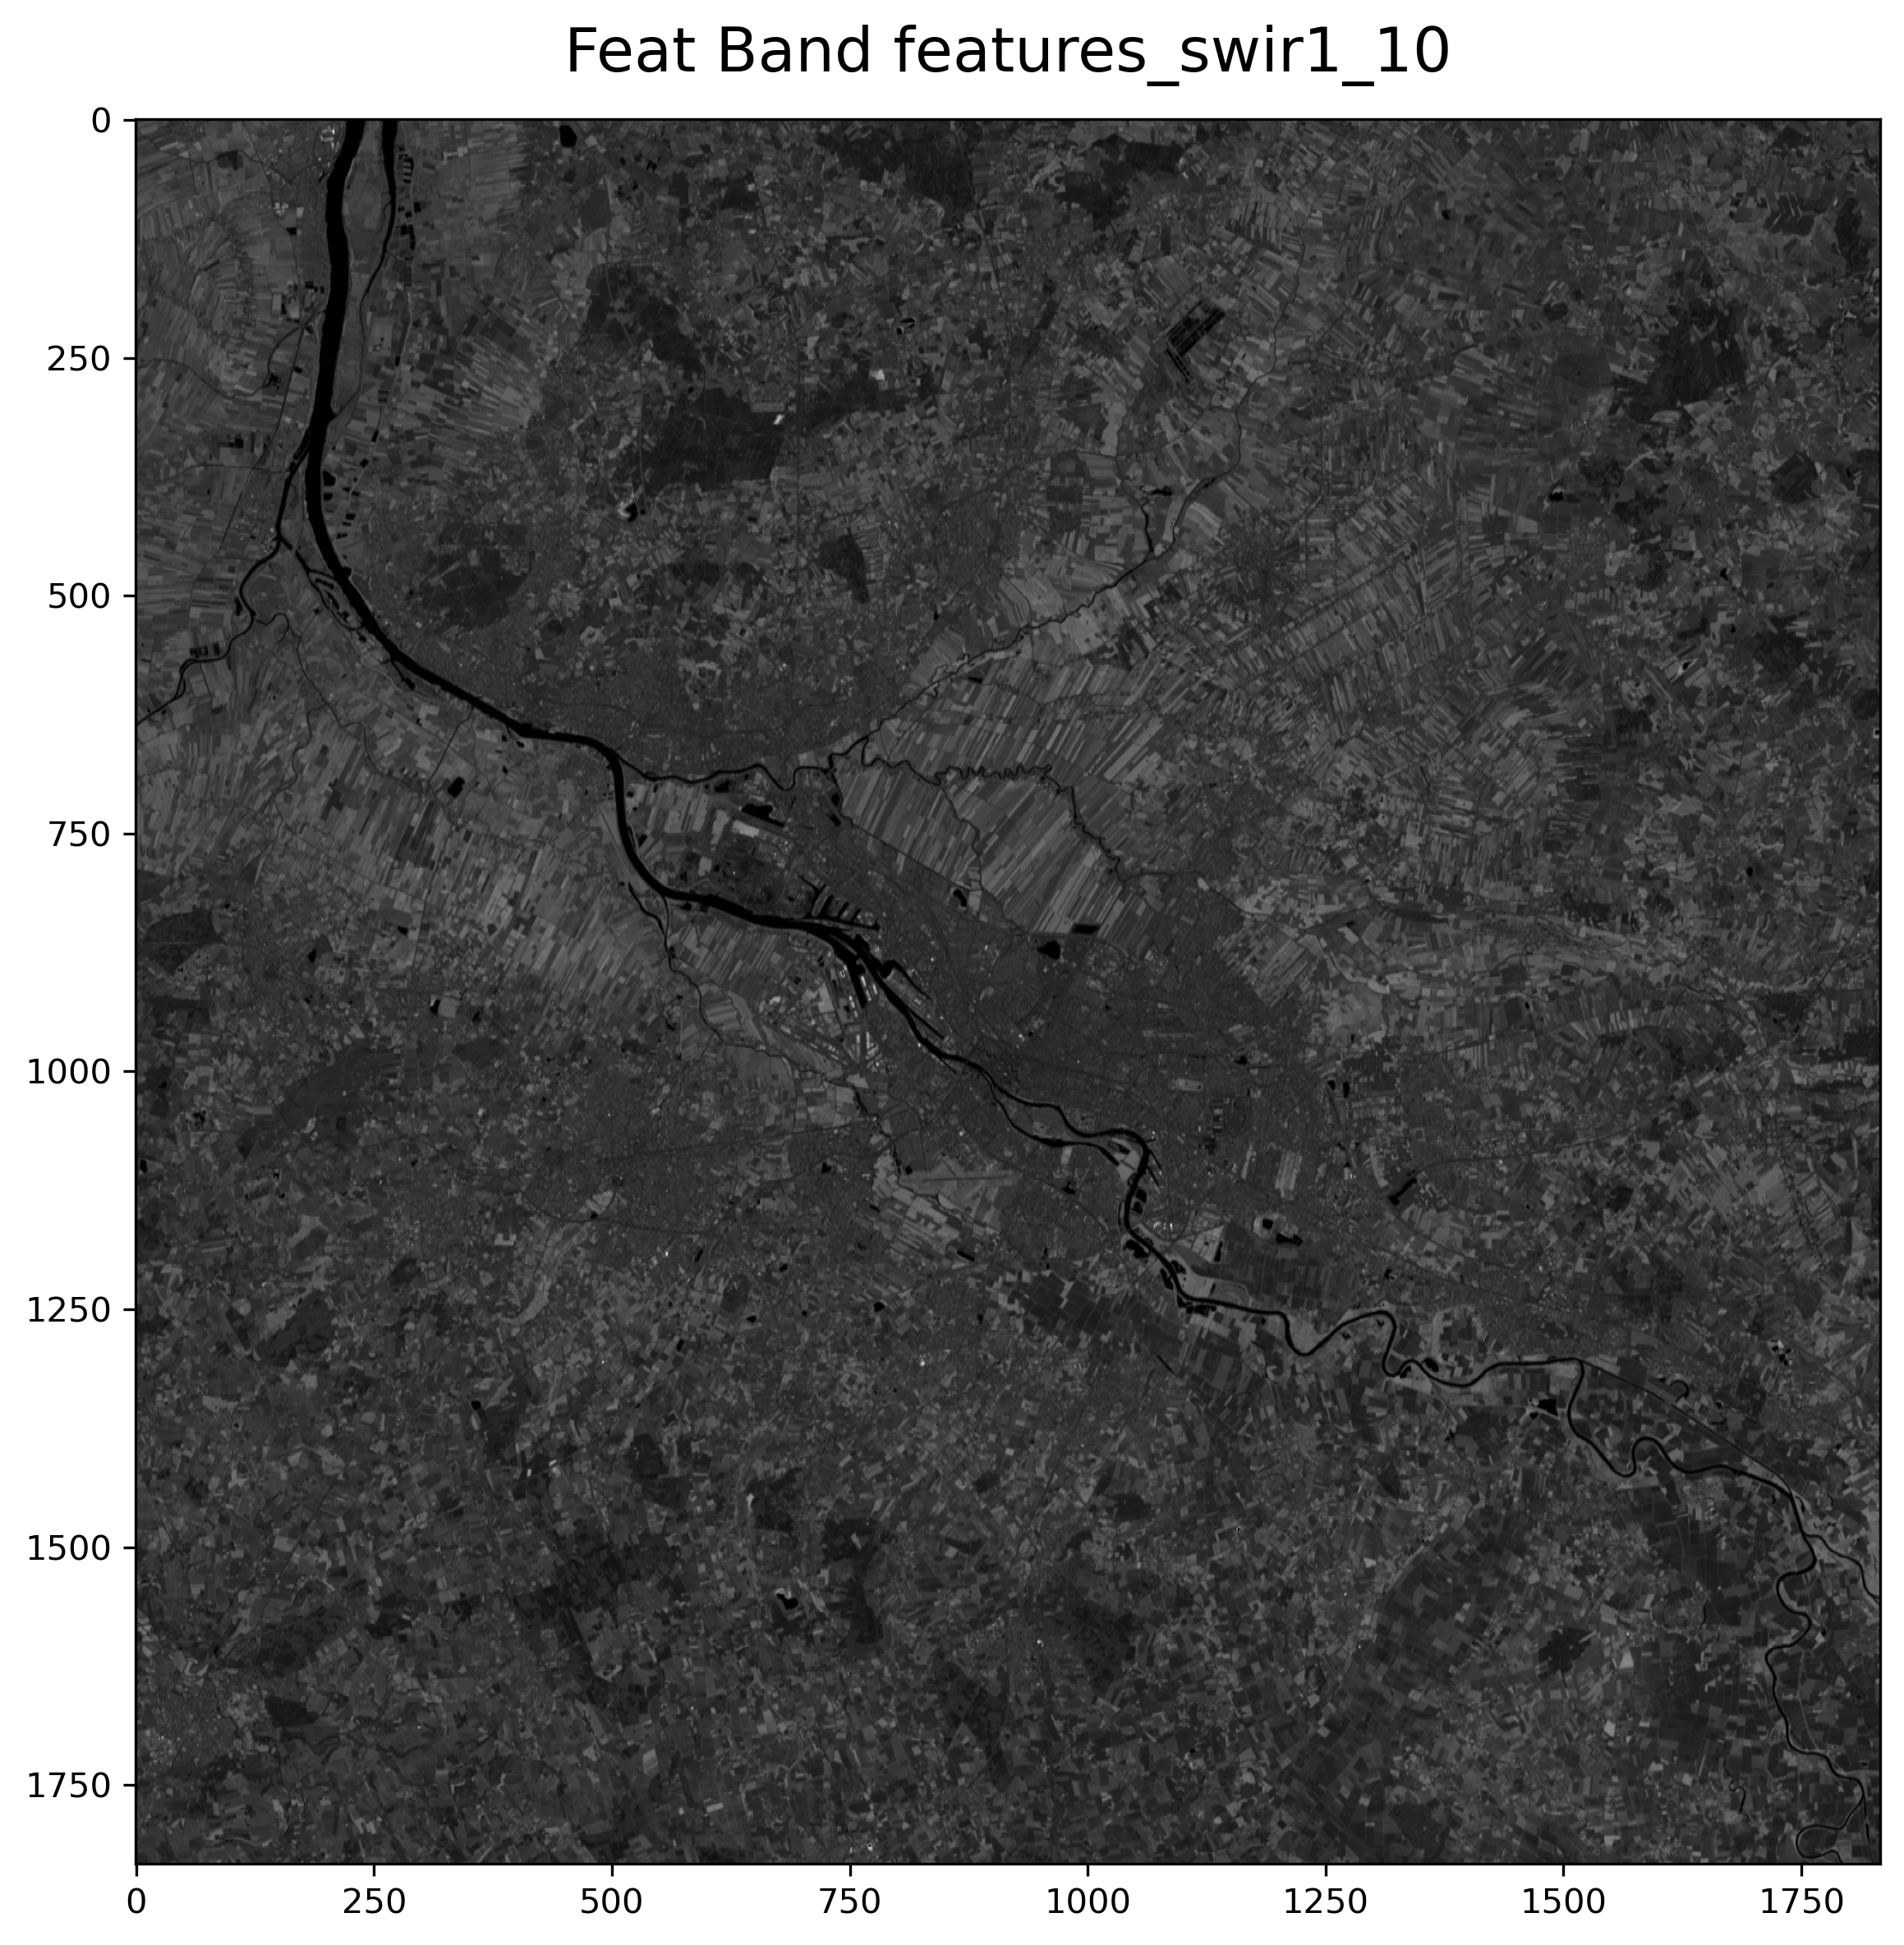
\includegraphics[width=\textwidth]{img/Features_swir10.png}
        \subcaption{Convolution of SWIR Band and kernel 10}
      \end{subfigure}
      \begin{subfigure}[b]{0.3\textwidth}
        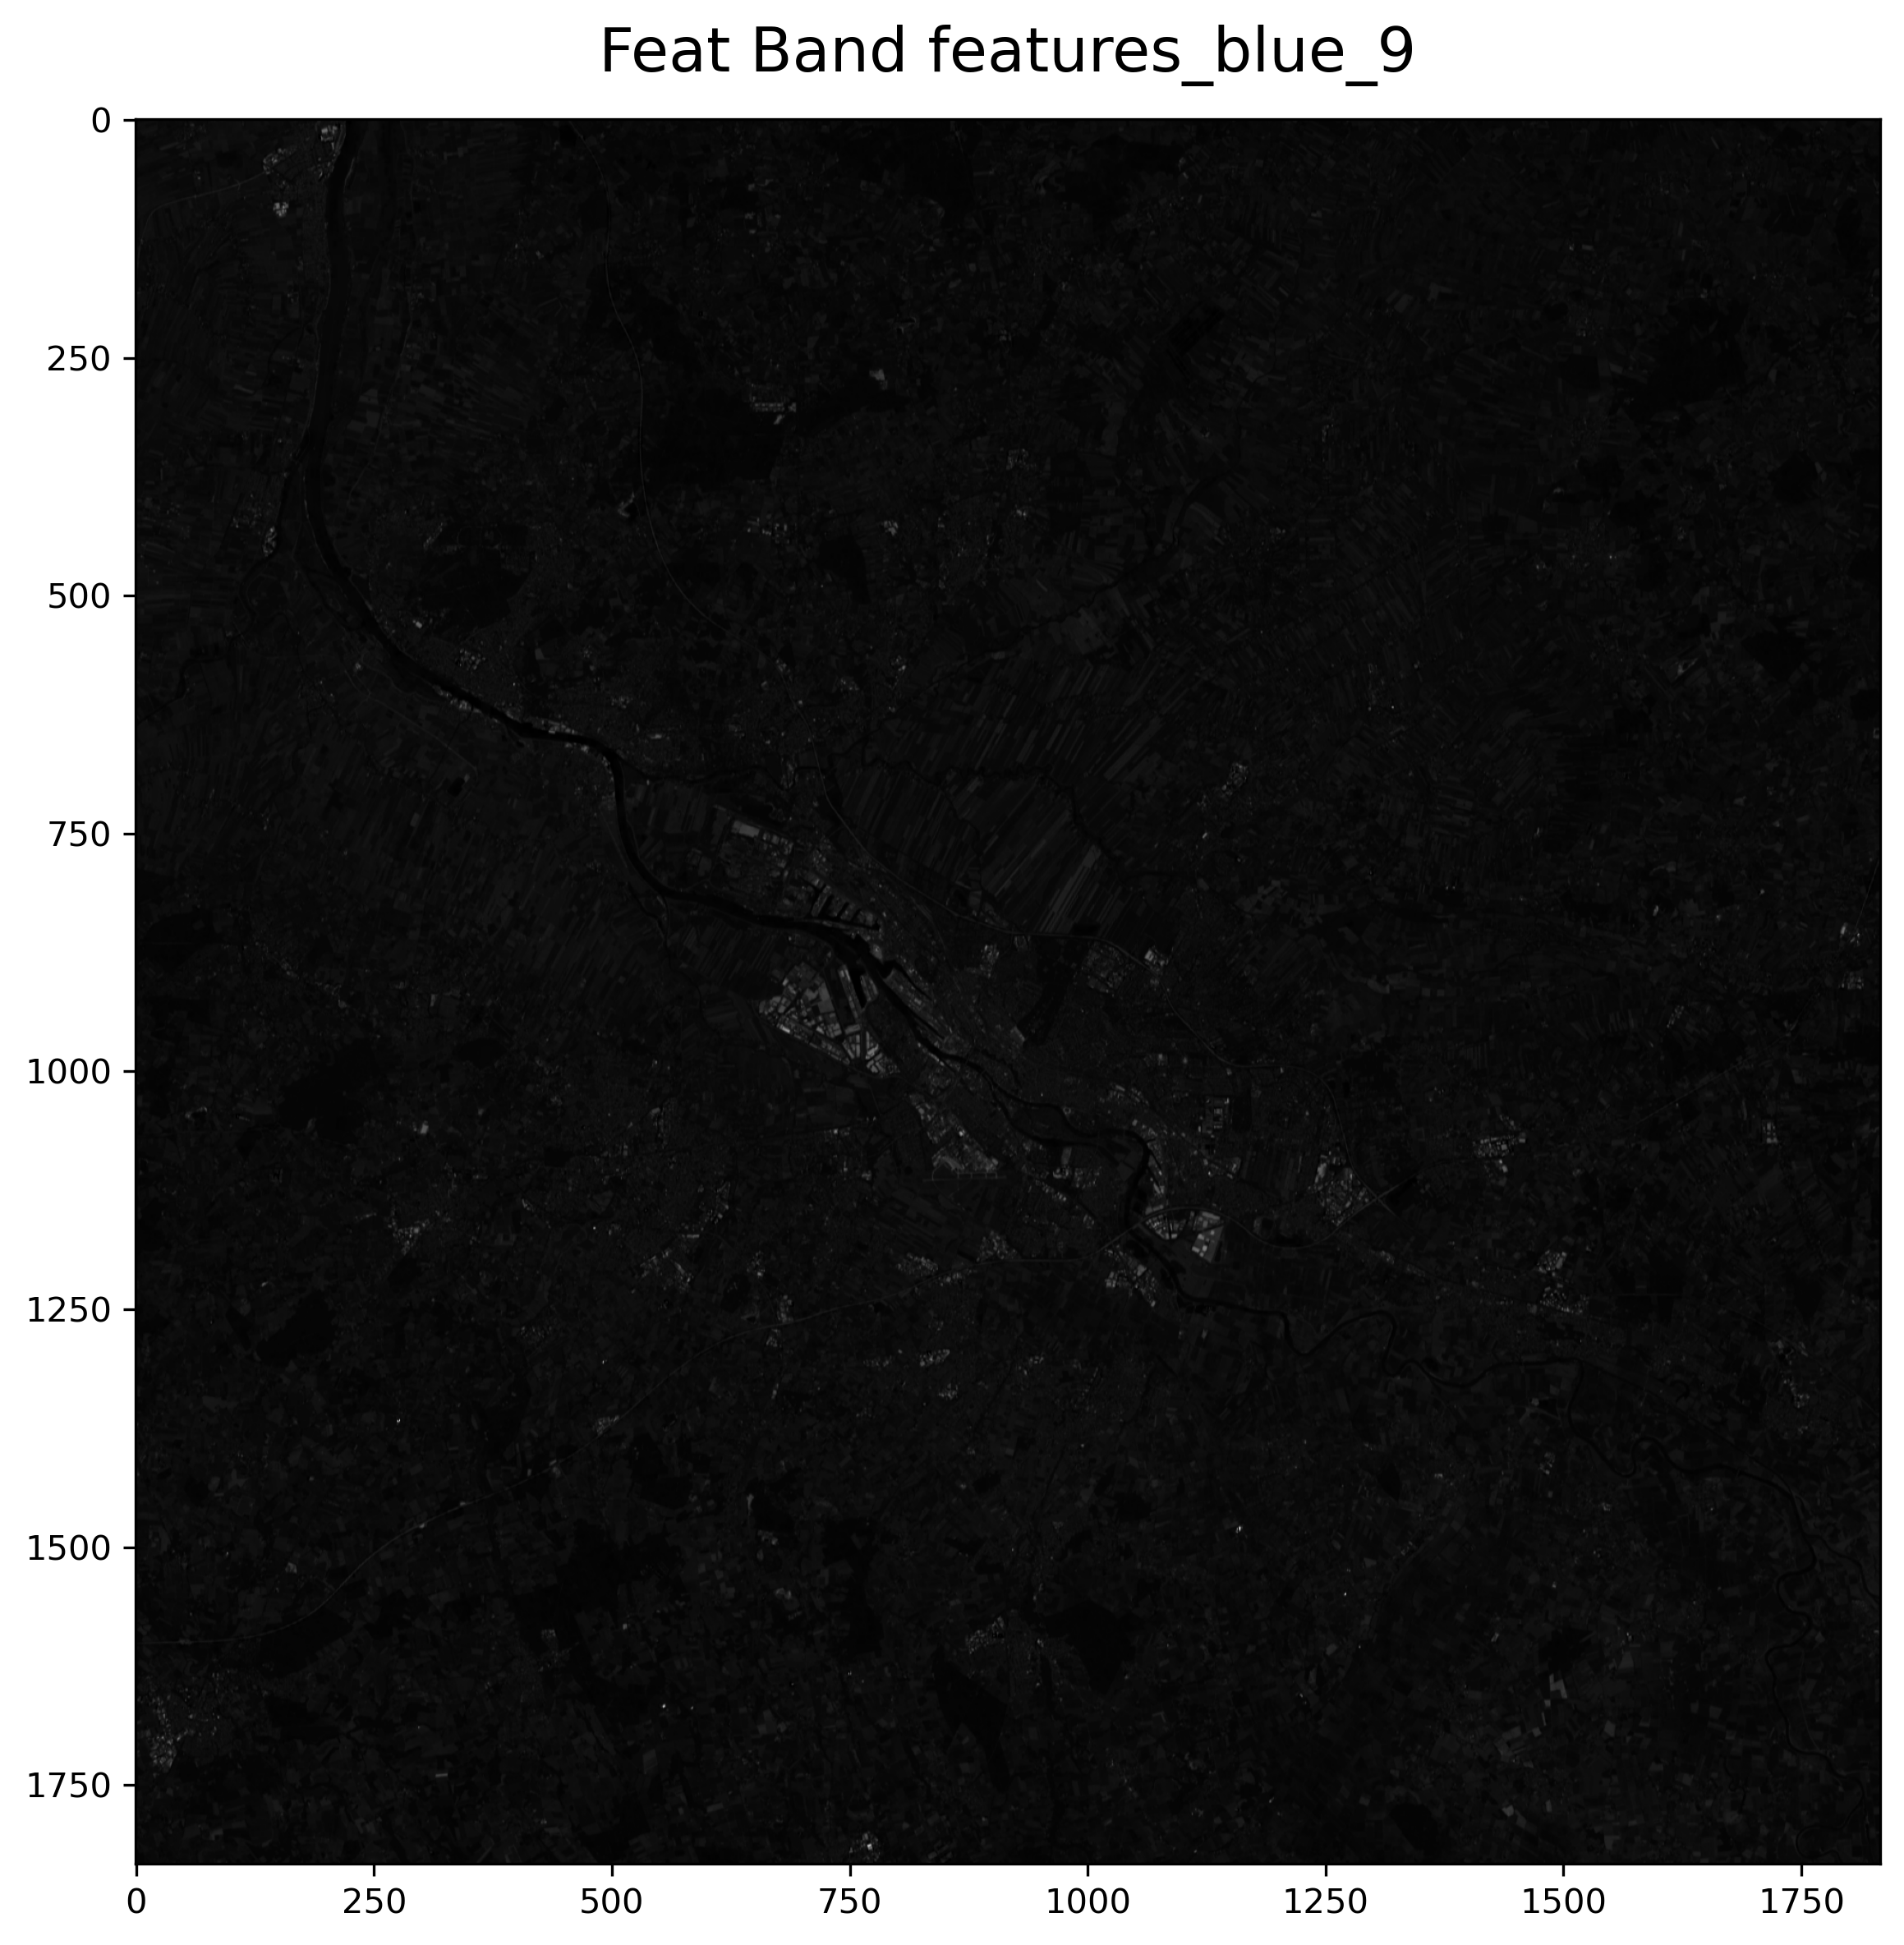
\includegraphics[width=\textwidth]{img/Features_blue3.png}
        \subcaption{Convolution of blue band and kernel 3}
      \end{subfigure}
      \begin{subfigure}[b]{0.3\textwidth}
        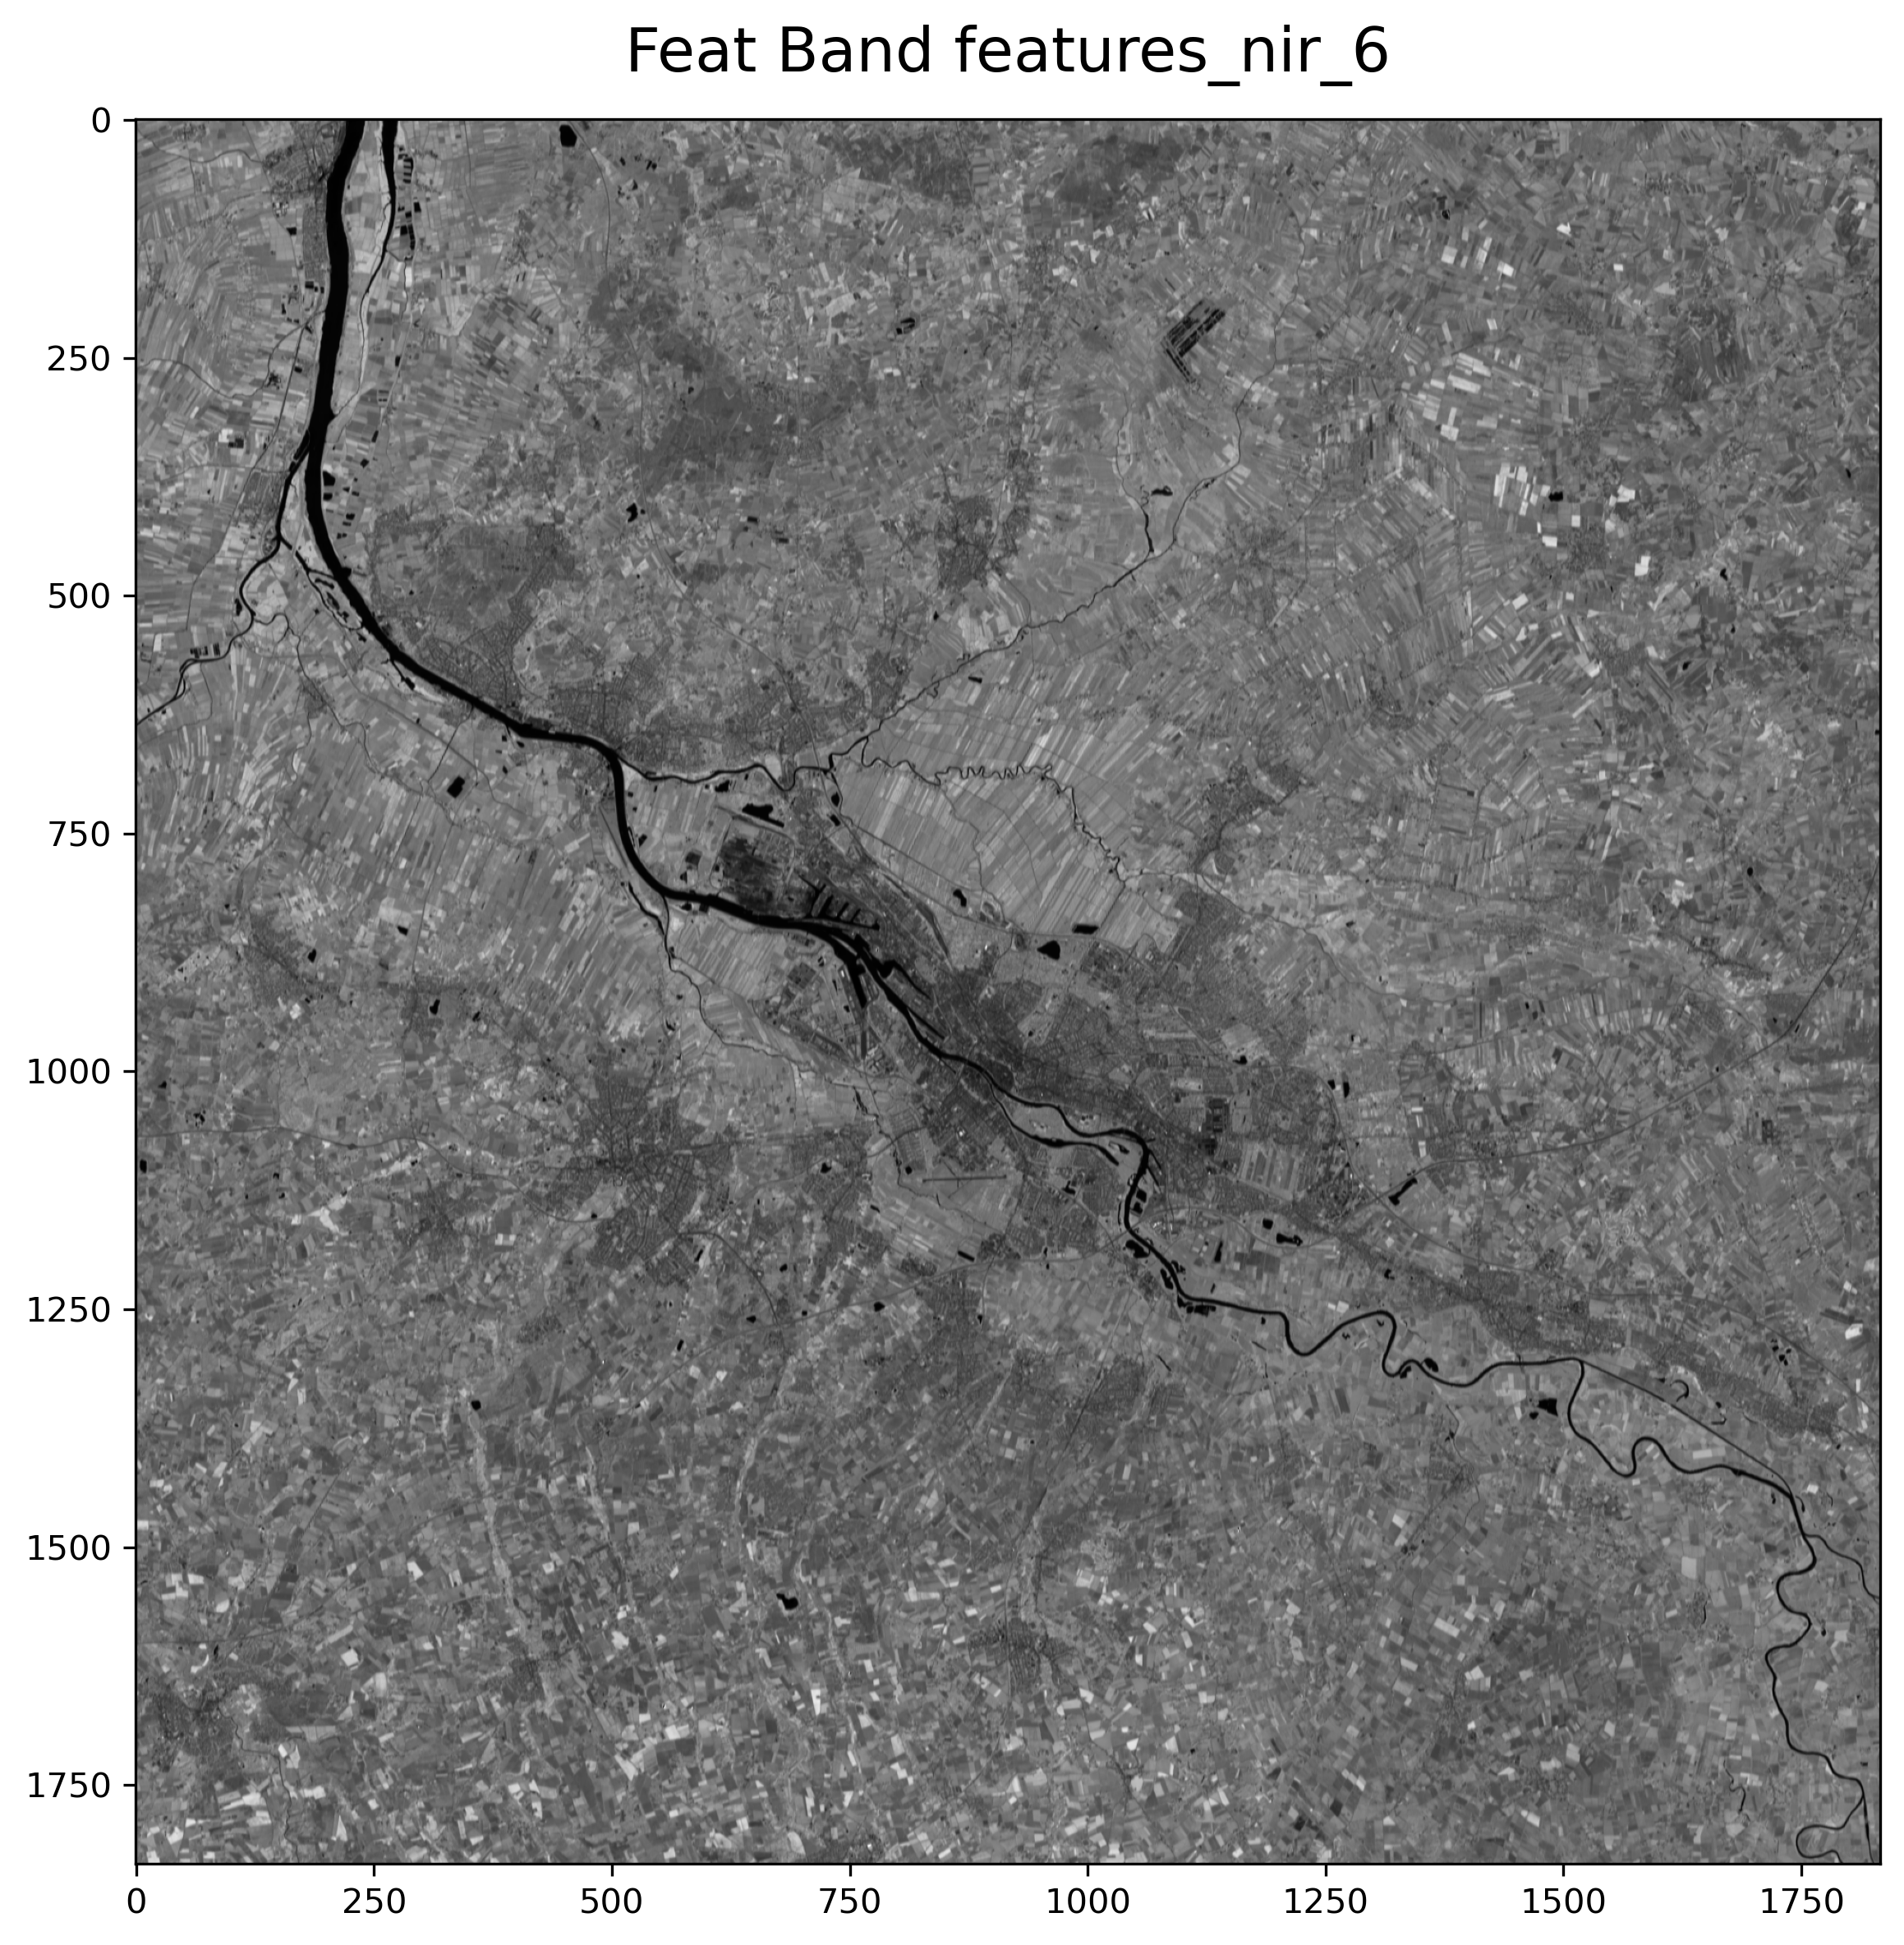
\includegraphics[width=\textwidth]{img/Features_nir_6.png}
        \subcaption{Convolution of NIR Band and kernel 6}
      \end{subfigure}
     \caption{Example feature images of the convolution of three bands and gabor filters \label{fig:gaborresults}}
    \end{figure}
 \noindent 
 %
      Each band of the image was then processed using a Gabor Feature Extraction algorithm with four rotations, parameter sets. 
      It was found, by variation of parameters, that the highest score was archived using 4 rotations of a symmetric kernel or 8 rotations of an asymmetric kernel with a 2:1 ratio.
      %TODO  verify
     % 
      %TOD TO find 
     % and (only circular kernel where used) with a $\lambda$ of 2 and 4. %TODO check 
      The optimal sigma was found using systematic variation to be between 1.0 and 1.5. 
      The frequencies of the sine wave where varied between 0.05 and 0.5. A trade-off between computation time and results was found using 3 frequencies shown in \cref{fig:gaborbank} \\ 
      This step was crucial in extracting and emphasizing spatial patterns and textures, thereby facilitating more distinct classification of land cover types. 
      %
      \begin{figure}
      \begin{subfigure}[b]{0.3\textwidth}
        \includegraphics[width=\textwidth]{img/red.png}
        \subcaption{Original Band}
      \end{subfigure}
      \begin{subfigure}[b]{0.3\textwidth}
        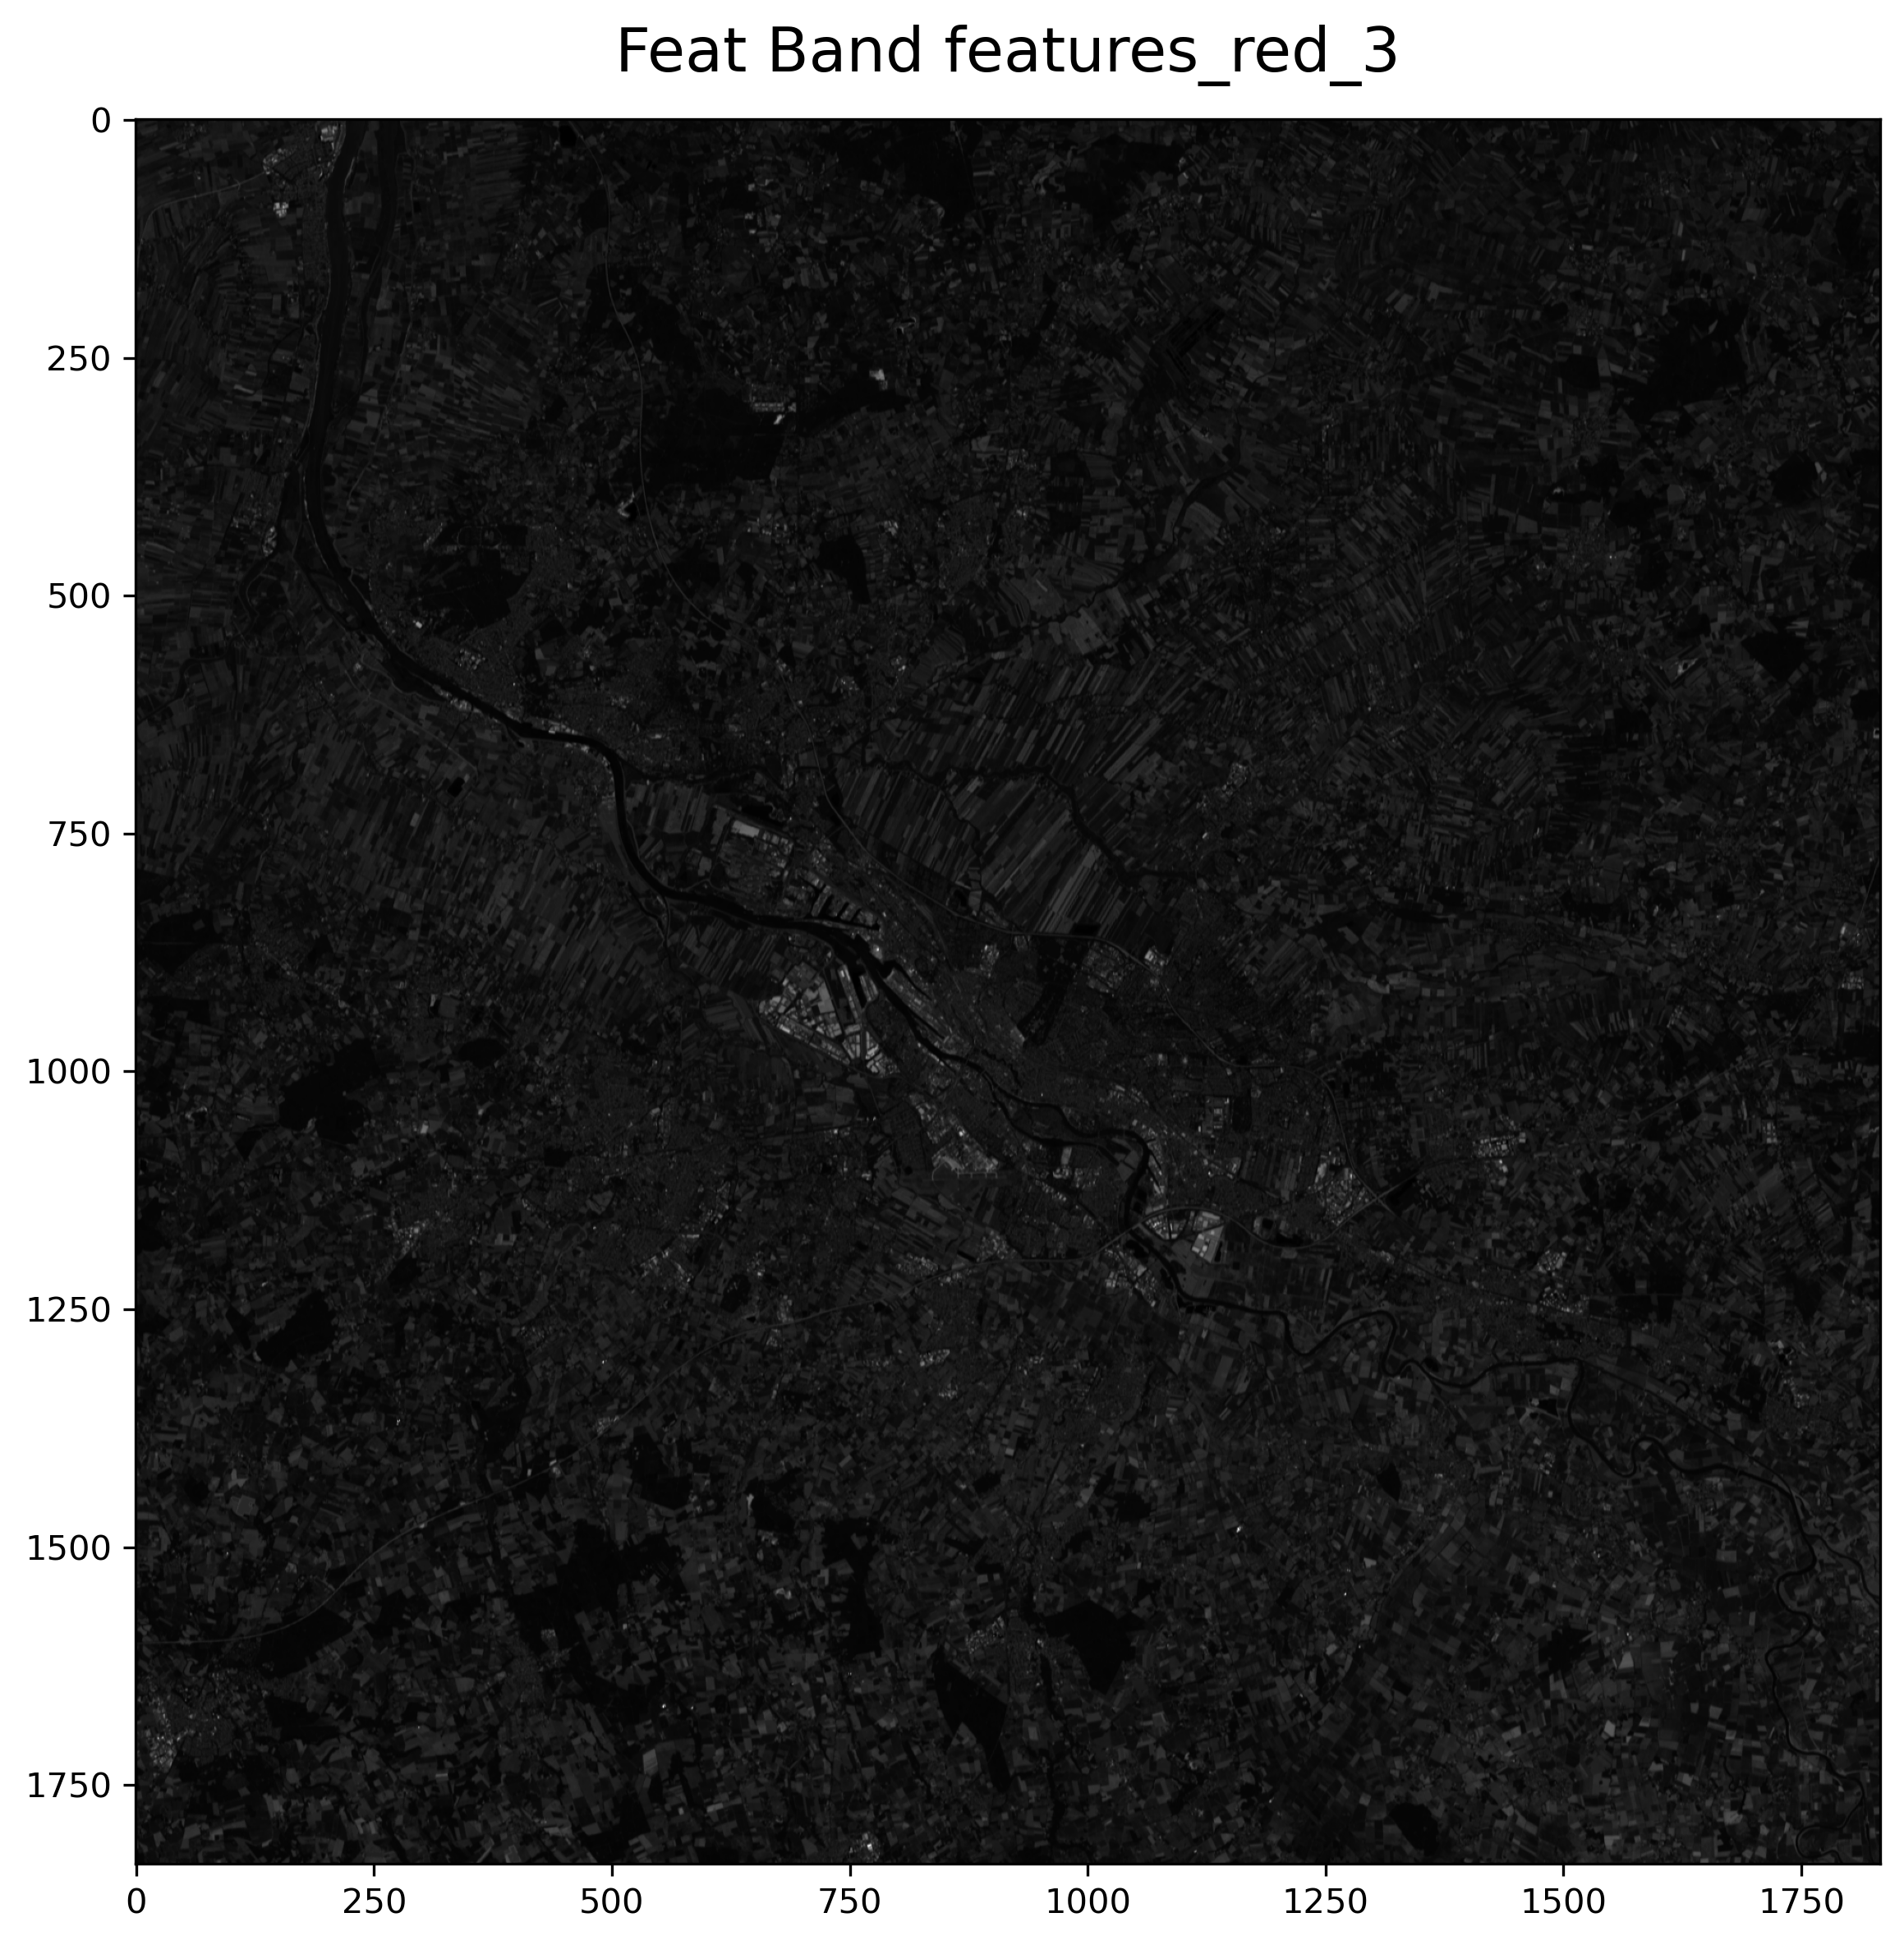
\includegraphics[width=\textwidth]{img/Features_red2.png}
        \subcaption{Convolution of NIR Band and kernel 6}
      \end{subfigure}
     \caption{Example feature images of the convolution of three bands and gabor filters \label{fig:gaborresults}}
    \end{figure}
      %TODO citation?
      For classifying surfaces an unsupervised machine learning was used. 
      %After the features were added the data was passed through the trained (random forest model \cref{sec:randomForrest}) for classification. \\
      The classified image has 11 classes that are shown in \cref{tab:land_cover_classes}
      \\
      The feature enhanced data of images of Bremen%, Valencia and TODO 
      were used of multiple years to create an unsupervised K-Means clustering model.%TODO add more 
      This initial clustering served as the foundation for the subsequent Random Forest machine learning model.
      The K-means algorithm was executed with varying numbers of classes – specifically 8, 10, and 11 – to determine the optimal classification schema.
      This model was validated using the Sentinel-2 10m Land Use/Land Cover map (\autocite{Zhang}).
      Since the data set only uses 8 classes, the used classes where mapped to the best fitting class (indicated in \cref{tab:land_cover_classes}). 
      clouds, cloud shadows and snow/ice where not used for verification and removed for the analysis.
      %TODO
      To judge results the output of the K-Means and the random forest was compared to the ESA CCI Land Use Dataset (~\autocite{landformclassicationusingfuzzykmeans2000}) that was scaled up to the used image resolution. %TODO check if correct reference
      \\
      TODO THE VALIDATION RESULTS STILL TBD~:/% 
      \\ 
      The Trained model was then used to classify other cities and datasets from different times. 
      Part of the training data as well as different time data from the same area was used and Feature enhanced using the same Gabor-Filter bank.
      Feeding the enhanced data into the random forests model was then used to determine the land cover classes for the next step of the analysis.
      \begin{table}[ht]
      \centering
      \renewcommand{\arraystretch}{1.4}
      \caption{Land Cover Classes Identified}\label{tab:land_cover_classes}
      \begin{tabular}{p{1cm}p{4cm}l}
      \toprule
      \textbf{Class Number} & \textbf{Land Cover Type} & \textbf{ESRI Class}\\
      \midrule
      1 &  Agricultural & Crops\\
      2 &  Bare Soil, Rock & Bare \\
      3 &  Vegetated Residential & Build Area\\
      4 &  Meadows & Crops\\
      5 &  Forest / Dense Vegetation & Trees \& Crops \\
      6 &  Residential & Build Area\\
      7 &  Fields & Crops\\
      8 &  Agricultural/ Fields & Crops\\
      %11 &  Residential/ Build-up& Build Area\\
      %8 &  Cloud Shadows & Clouds \& Any \\
      %9 &  Fields and meadows& Rangeland \&Crops \\
      %10 &  & Clouds \\
      9 &  Industry Halls & Build Area\\
      10 &  Agricultural (2) & Crops\\
      11 &  Water& Water / Flooded Vegetation\\
      \bottomrule
      \end{tabular}
      \end{table}

      %For the labelling of these land cover classes, the Normalized Difference Vegetation Index (NDVI) and the Normalized Difference Built-up Index (NDBI) bands were utilized.
      %These indices were instrumental in differentiating vegetated areas from built-up regions, thereby aiding in the accurate categorization of land cover types.
      The classification labels were assigned based on the proximity of the cluster centres of the trainings data to the cluster centres of the K-means fit.
      This approach ensured that each land cover class was consistently labelled independent of the study area.\\
    %
    \subsubsection{Urban Area Extraction}
      The resulting classified image was then processed to extract urban areas.
      The algorithm used the classes 1,2,6 and 11 from \cref{tab:land_cover_classes} to detect areas that can be considered urban.
      The areas were \gls{dilated} and \gls{eroded} to bridge small gaps between parts of the city and close holes as well cut small thin links such as highways between larger areas.
      After this preprocessing step the areas are enumerated and all areas that cover at least 1\% of the image area where used to create buffer zones. 
  
      Bufferzones where defined as described in \cref{sec:urbanBufferzone}.\\
      TODO add images or code snippet
 \subsection{Analysis}\label{sec:landcoverAnalysis} 
  The output of the land cover classes was compared with the CCI Sentinel-3 based land cover product. This product has a 300 m resolution but an upscaling and downscaling was done to get the data

 \subsection{Conclusions}
    In summary, the integration of enhanced Landsat imagery, Gabor filtering, K-means clustering, and Random Forest classification constituted a robust methodology for land cover classification.
    This process not only facilitated a detailed and accurate representation of the study area's land cover but also demonstrated the efficacy of combining various remote sensing and machine learning techniques for environmental analysis.
    The number of classes that are distinguishable for the algorithm highly varied so it a possible improvement would be the use of reducing machine learning algorithms, that identifies the principle components between c.
    %
  \newpage
  \section{Impact of Climate Change on Urban Heat Islands}\label{sec:UHITempImp}
    \subsection{Introduction}
       The interaction between global and local climate is a complicated process that has multiple parameters, that are not completely understood nor are they all easily measurable. 
       In central Europe the climate is governed by seasonality typical for the northern hemisphere.  
       According to multiple studies global rise of temperature due to climate change is also increasing temperatures in northern Europe~\autocite{Benestad2005}  %TODO this is not really what I want...

       %A climate tipping point (see~\autocite{Lenton2008}) that could cause severe cooling in northern Europe is the breakdown of the Atlantic Thermohaline circulation\cite{Rahmstorf1999}.
       %TODO add a sentence for why
       %But since the European climate is still under influence by the warm ocean currents, 
       The temperatures in major European cities have increased at a similar pace then the global mean temperatures. 
       The cities covered by this study observed an average increase from 1990 to 2020 of %TODO 
       \textdegree\ C. 
   
       The hypothesis is that the rising temperatures observed over the past 30 years have increased heat island severity and size. 
    \subsection{Methodology}
      Measurement of the impact on rising temperatures have to be done after correcting for other variables such as urban development, meteorological impact factors such as wind and rain. 
      To archive this a time series of land surface temperatures and \glspl{UHI} from 1990 to 2022 was created using Landsat 7 and Landsat 8 and 9 data.
      Data from weather stations in the areas where used to calculate the trend of mean temperature over the time. 
      The \glspl{UHI} data was then correlated with the air temperature data of the local measurement stations and corrected for size increases of \gls{UHI} impacted by land cover change in the previous step. 
      This way in the statistical analysis all \glspl{UHI} that would be impacted by urbanisation or change of surface type where excluded from the analysis.
    \subsubsection{Data Handling}
      One of the challenges that arised during the processing of multiple images where the large amount of data of the images (each fully loaded image with all 11 bands including classification is around 1.5 GB).
      To reduce the memory footprint of the processing chain, xarray (\autocite{hoyer2017xarray}) was used. 
      Xarray allows lazy loading from disk, this only loads parts of the complete data set. 
      Another feature of xarray that was used are labelled data. Each loaded image used latitude and longitude as coordinates allowing to accessing sub areas by reference coordinates. 
      Another axis was added for the time dimension, so that each area could be stored in a single data file, but access is done loading only the relevant data for a specific time or a selected time frame.
  
      For this step the following data was loaded from the previous dataset: 
      \begin{itemize}
        \item Band data from the area of interest (Band 1 to 10)
        \item Classification label, a layer with the numerical classifications assigned to each pixel 
        \item Urban mask, a layer with urban, suburban and peri-urban areas
        \item \glspl{UHI}, for each time step a layer, masking urban heat islands
      \end{itemize}
    \subsubsection{Land Surface Temperature Calculation}\label{sec:lstcalc}
      The \gls{LST} can not be measured directly by a satellite but must be calculated from the upwelling thermal infrared radiation and corrected for the atmospheric perturbation. 
      For Landsat 7 and Landsat 8 data is provided in different processing levels.
      For analysis of past data that has already be processed the level 2 data can be used, that provides land surface temperature and has been calculated from the level 1 data. 
      To derive the level 2 data from level 1 data, \gls{TOA} brightness is used, corrected for stray light (Landsat 8 specific, see~\autocite[p.~67]{Zanter2019}) and instrument distortion. Then geometric and geographic terrain-correction (\cite[p.~44]{Zanter2019}) is applied..
      The \gls{TOA} temperature data is calculated according to \cref{equ:toa} where $K_1$ and $K_2$ are band specific conversion factors from the meta data file and $L_\lambda$ is the spectral radiance at the TOA in $\frac{W}{m^2\cdot srad \cdot \mu m}$ e.g.\ the Band 10 Channel. 
      \begin{equation}\label{equ:toa}
  	    T = \frac{K_2}{\ln\left(\frac{K_1}{L_{\lambda}}+1\right)}
      \end{equation}
      To get the level two data from these \glspl{TOA} measurements the value is corrected for emissivity of the ground using measurements from the \textit{ASTER GED} database (see~\autocite{USGSWebsite}).\\
      The temperature is also corrected for atmospheric interference using local reference stations. 
      The USGS uses reference stations, atmospheric models and independent reference measurements from other satellites to calculate the Surface temperature, the surface temperature product has an accuracy of $\pm 1 K$ overall and other uncertainties are marked in a quality assurance file provided for each image.\\
      To convert the image file containing 16 bit unsigned integers into a temperature \cref{equ:tiftolst} is used, where DN is the integer value. The scaling and offset factors are specific to the product and where taken from~\autocite{EROASC2013}.
  
      \begin{equation}\label{equ:tiftolst}
        T_C = T_K -273.15 = \frac{DN}*0.00341802 + 149.0 - 273.15 
      \end{equation}
  
      The Temperature was then converted back into an integer to reduce storage requirements, this is not degrading calculations, since the accuracy of the temperature product is lower then $\pm 1$°C.
  \newpage
    \subsubsection{Calculating temperature rise within the city}
      For the city in question the next ground based measurement stations where used to calculate a fitted temperature regression. 
      This data % TODO add image 
      was correlated with the \gls{SUHI} intensity as well as the measured temperature data from the times of the satellite data acquisitions. 
      For German cities the stations of the \gls{DWD} where used.
      %#Using the~\autocite{wetterdienst2024} library, that allows locating the nearest weather station having sufficiently high resolution weather data. 
      One indicator interesting in the research on \glspl{UHI} is the number of days with high temperature.
      There are multiple threshold days that are used to classify seasons in comparison to the average.
      Hot days (defined by the \gls{DWD} as days with a maximum temperature over 30 °C), summer days (maximum temperature over 25 °C) and tropical nights (days with daily minimal temperature over 20 °C), are tracked by metrological organisations~\autocite{dwdklimalexikon}.
      Another measurement to visualize a rise in average temperature is the amount of frost days (where the minimal temperature is below 0 °C). 
      \subsection{Analysis}\label{sec:tempanalysis}
  
  \subsubsection{Bremen}
  Bremen was selected as the base area of the study, to be able to verify classification results and due to personal local knowledge. 
  The study area covers the city centre of Bremen and an area of 27 km in all directions covering an area of approximately $3000\ km^2$. 
  The study area is at sea level elevation and has a temperate-oceanic climate according to the~\autocite{koppen1930handbuch} classification.% and it's location is shown in .
    \begin{figure}[!htbp]
     \centering
        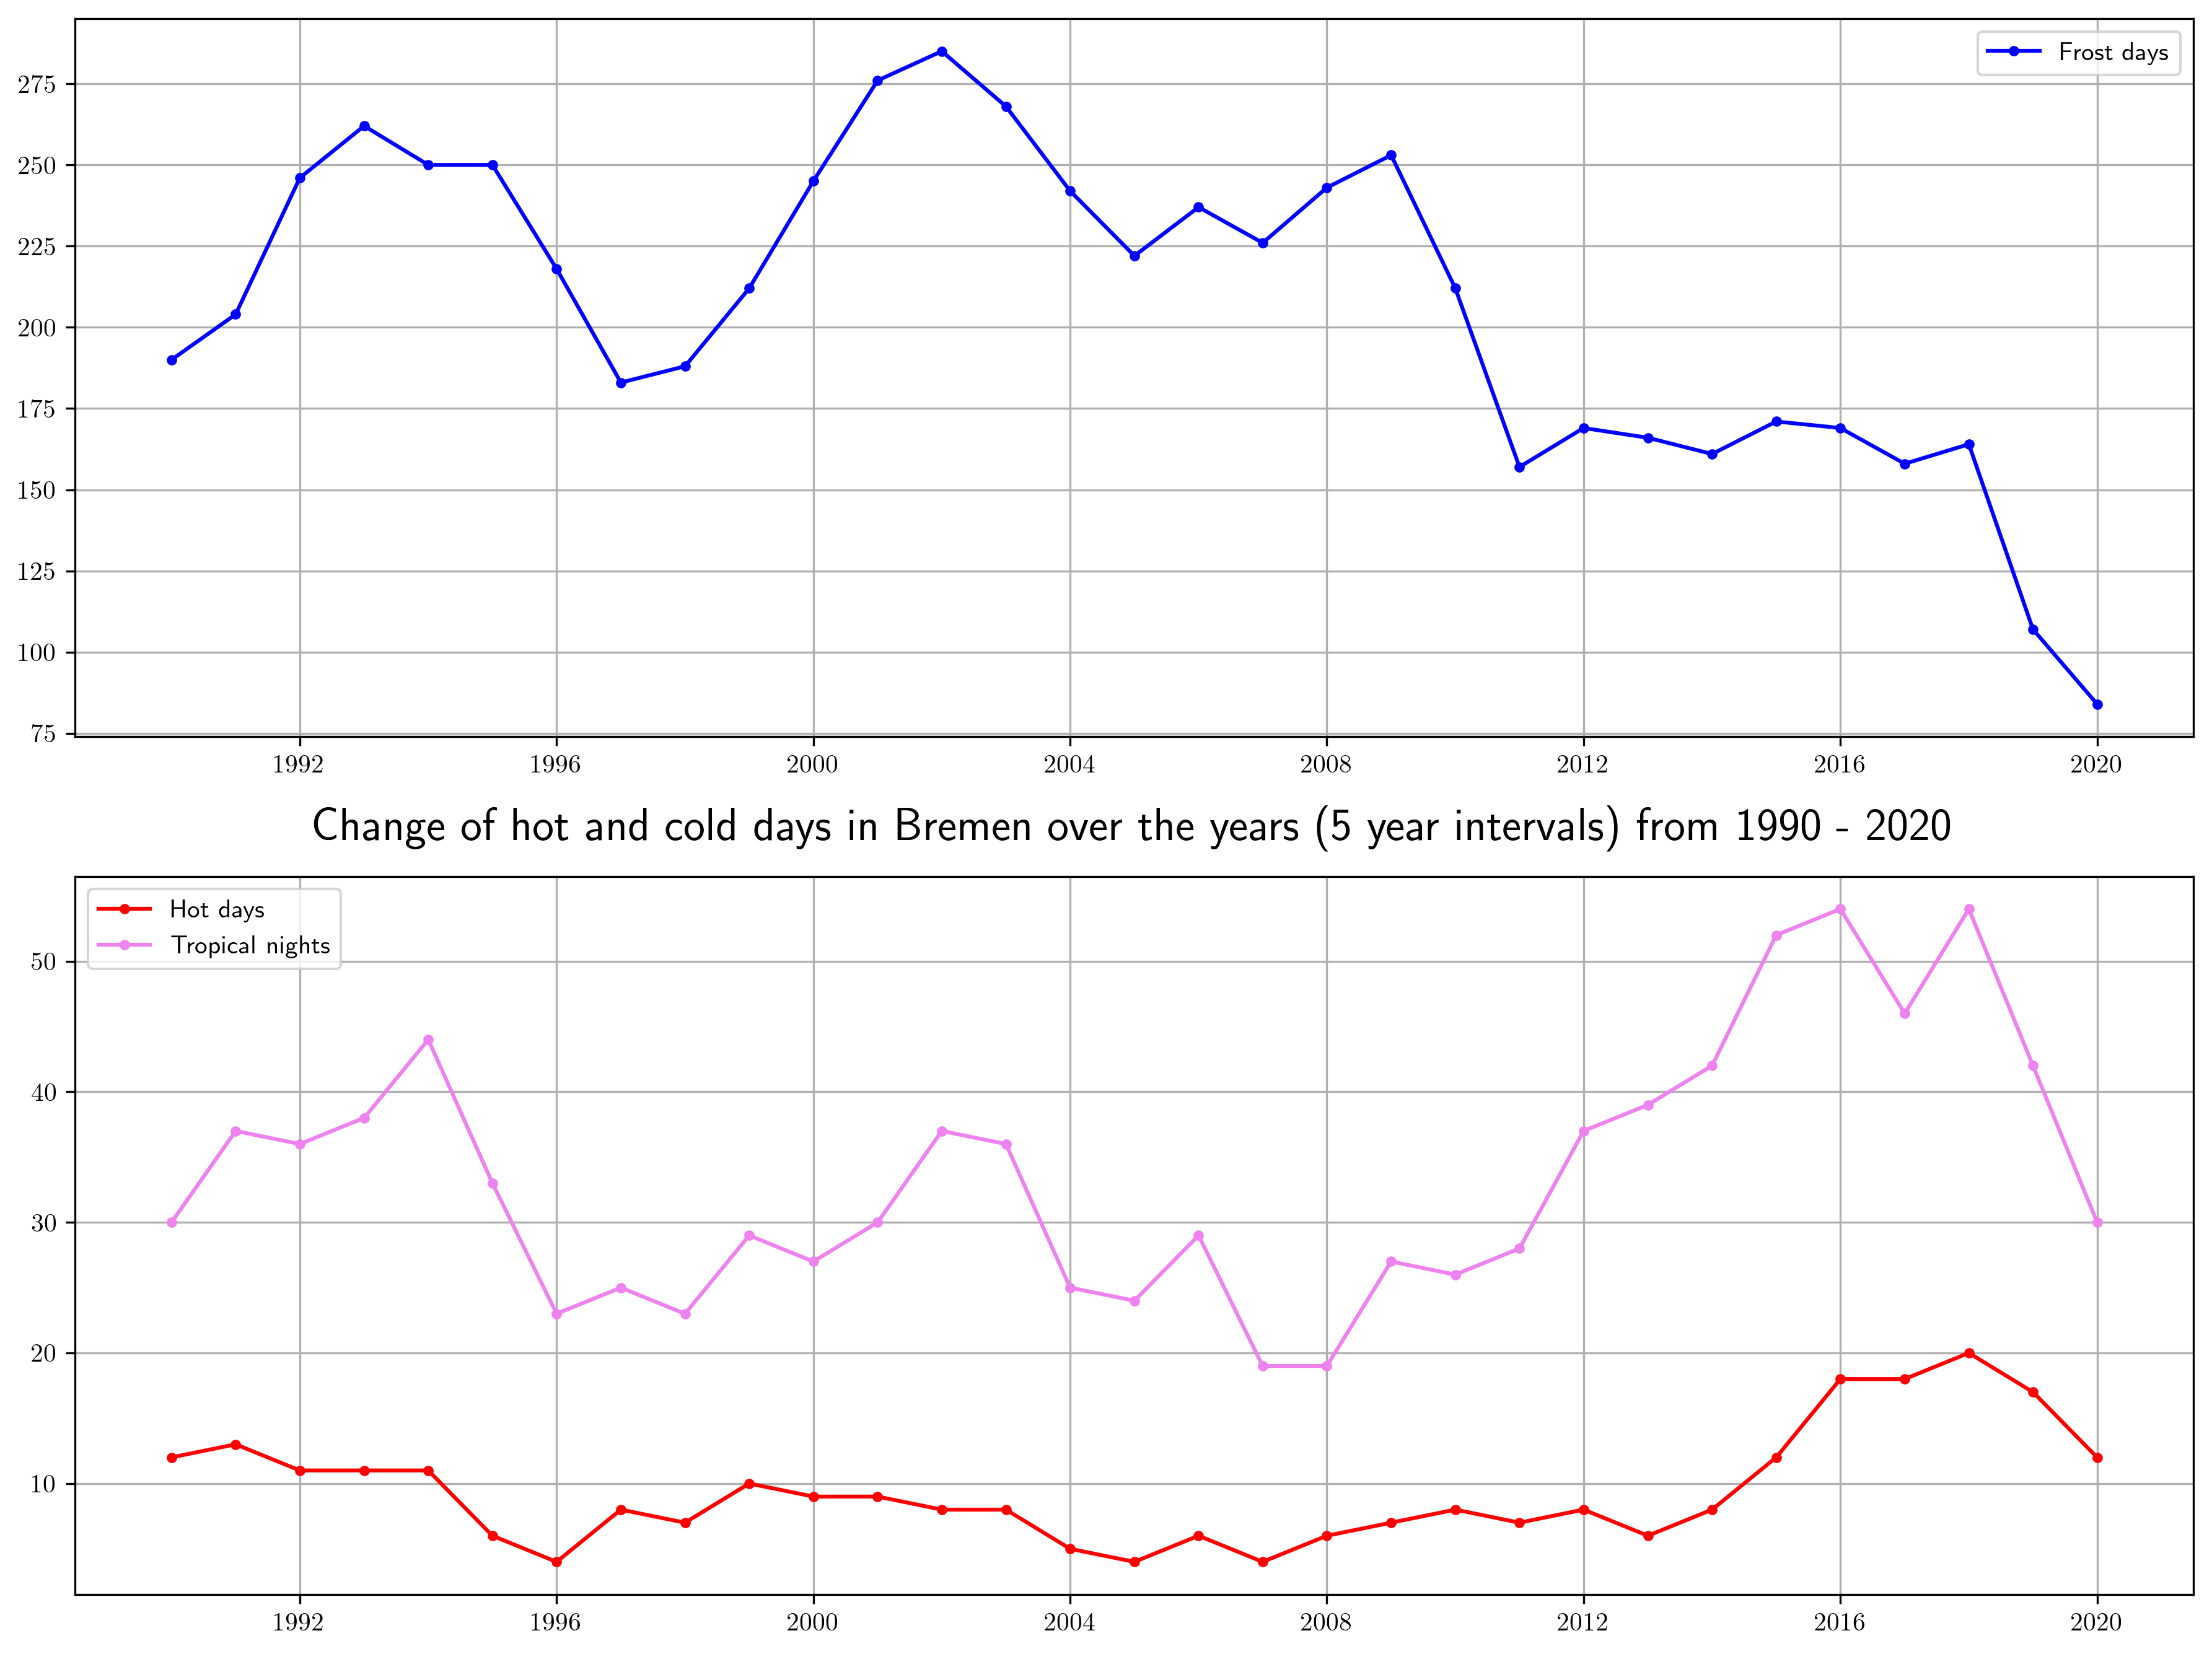
\includegraphics[width=\textwidth]{img/BremenKIChanges}
        \caption{Development of threshold days over time\label{fig:climateovertimeBremen}}
   \end{figure}
   An overview of the climate of Bremen is shown in \cref{tab:statsBremen}.
  \begin{table}[ht]
    \centering
    \caption{Bremen weather data using~\autocite{DWD2024a} data\label{tab:statsBremen}}
  \renewcommand{\arraystretch}{1.4}
    \begin{tabular}{p{3.5cm}p{2.5cm}lp{2.5cm}}
      \toprule
      & \textbf{Extremly Cold} & \textbf{Average} & \textbf{Extremly Warm} \\
      & min & mean & max \\
      \midrule
      Annual average °C \newline (Jahr)     &   7.2 \newline(1940)       & 9.4    & 11.1\newline (2020)      \\
      Abs. T °C \newline (Jahr)             & -23.6 \newline(Feb. 1940)  &        & 37.6 \newline(Aug. 1992) \\
      Summer days \newline($T_{\max}~\ge$  25 °C) & 4                    & 27.7   & 78 \\
      Hot days \newline($T_{\max}~\ge$  30 °C)    & 0                    & 4.9    & 22 \\
      \midrule
      & max & mean & min \\
      \midrule
      Frost days \newline($T_{\min}~<$  0 °C)     & 105         & 70.8   & 24 \\
      Ice days \newline($T_{\max}~<$  0 °C)       & 54          & 14.9   & 0  \\
      \bottomrule
    \end{tabular}
  \end{table}
%
   The threshold days over time are shown in \cref{fig:climateovertimeBremen},
   The weather station in Bremen is located at the airport on the edge of the city area. %TOOD image? 
   For comparison of air temperature with a more rural area the \gls{DWD} weather station ``Worpswede-Hüttenbusch'' located roughly 30 km north-north-east of the weather station and is located in a rural area. 
   To verify that the measurements of the urban and rural stations are correlated the absolute temperature difference for daily values is shown in \cref{fig:diff2015Bre} and \cref{fig:diff20222Bre}, it can be seen that the atmospheric \gls{UHI} over Bremen is affecting the Bremen airport station. 
   In the period from April to October in 2015 the daily mean temperature was 0.6 °C lower at the rural station. 
%
   In the same period in 2022 the daily mean temperature was 0.85 °C lower at the rural station. 
   %TODO add min and max and reason for why it is like that 
%
%  
%
   %TODO for the days show a plot with both measurements (rural/ urban) 
    \begin{figure}[!p]
     \centering
       \begin{subfigure}[b]{\textwidth}
         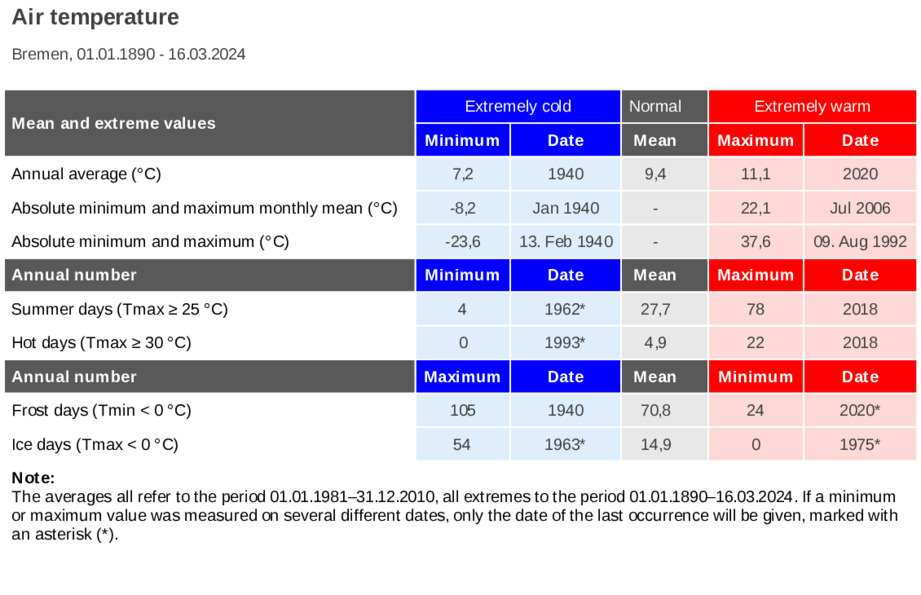
\includegraphics[width=\textwidth]{img/DWDBremenWeather.jpg}
         \subcaption{Weather in Bremen with key threshold days~\autocite{DWD2024a}\label{fig:bremenclimateoverview}}
       \end{subfigure}

       \begin{subfigure}[b]{\textwidth}
        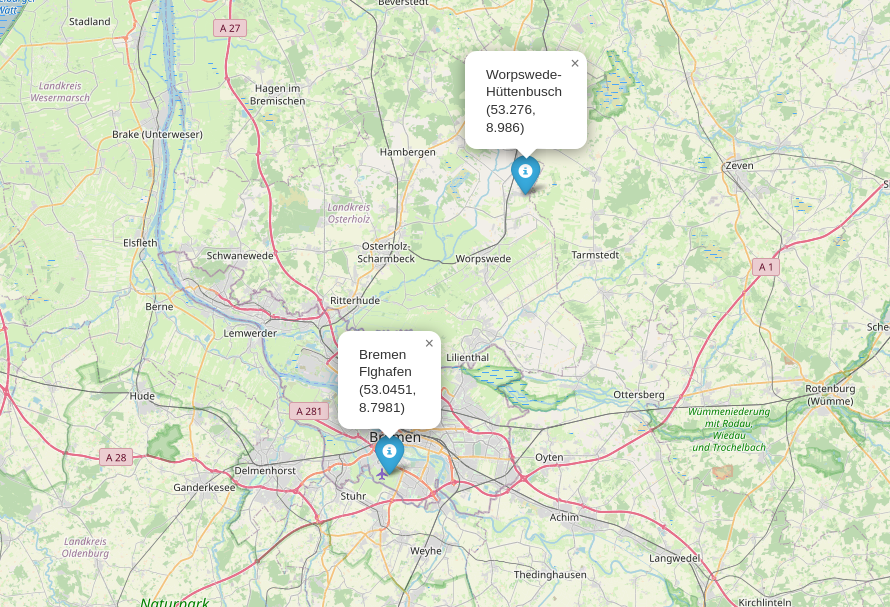
\includegraphics[width=\textwidth]{img/MapWetterstationenBremen.jpeg}
         \subcaption{Location of the weather stations in Bremen and the rural reference station in Worpswede-Hüttenbusch}\label{fig:mapWeatherstationsBremen}
       \end{subfigure}
         \caption{Overview of the data used for the analysis of the Bremen \glspl{UHI}}\label{fig:AnalysisBre}
   \end{figure}
%
    \begin{figure}[!p]
     \centering
       \begin{subfigure}[b]{\textwidth}
        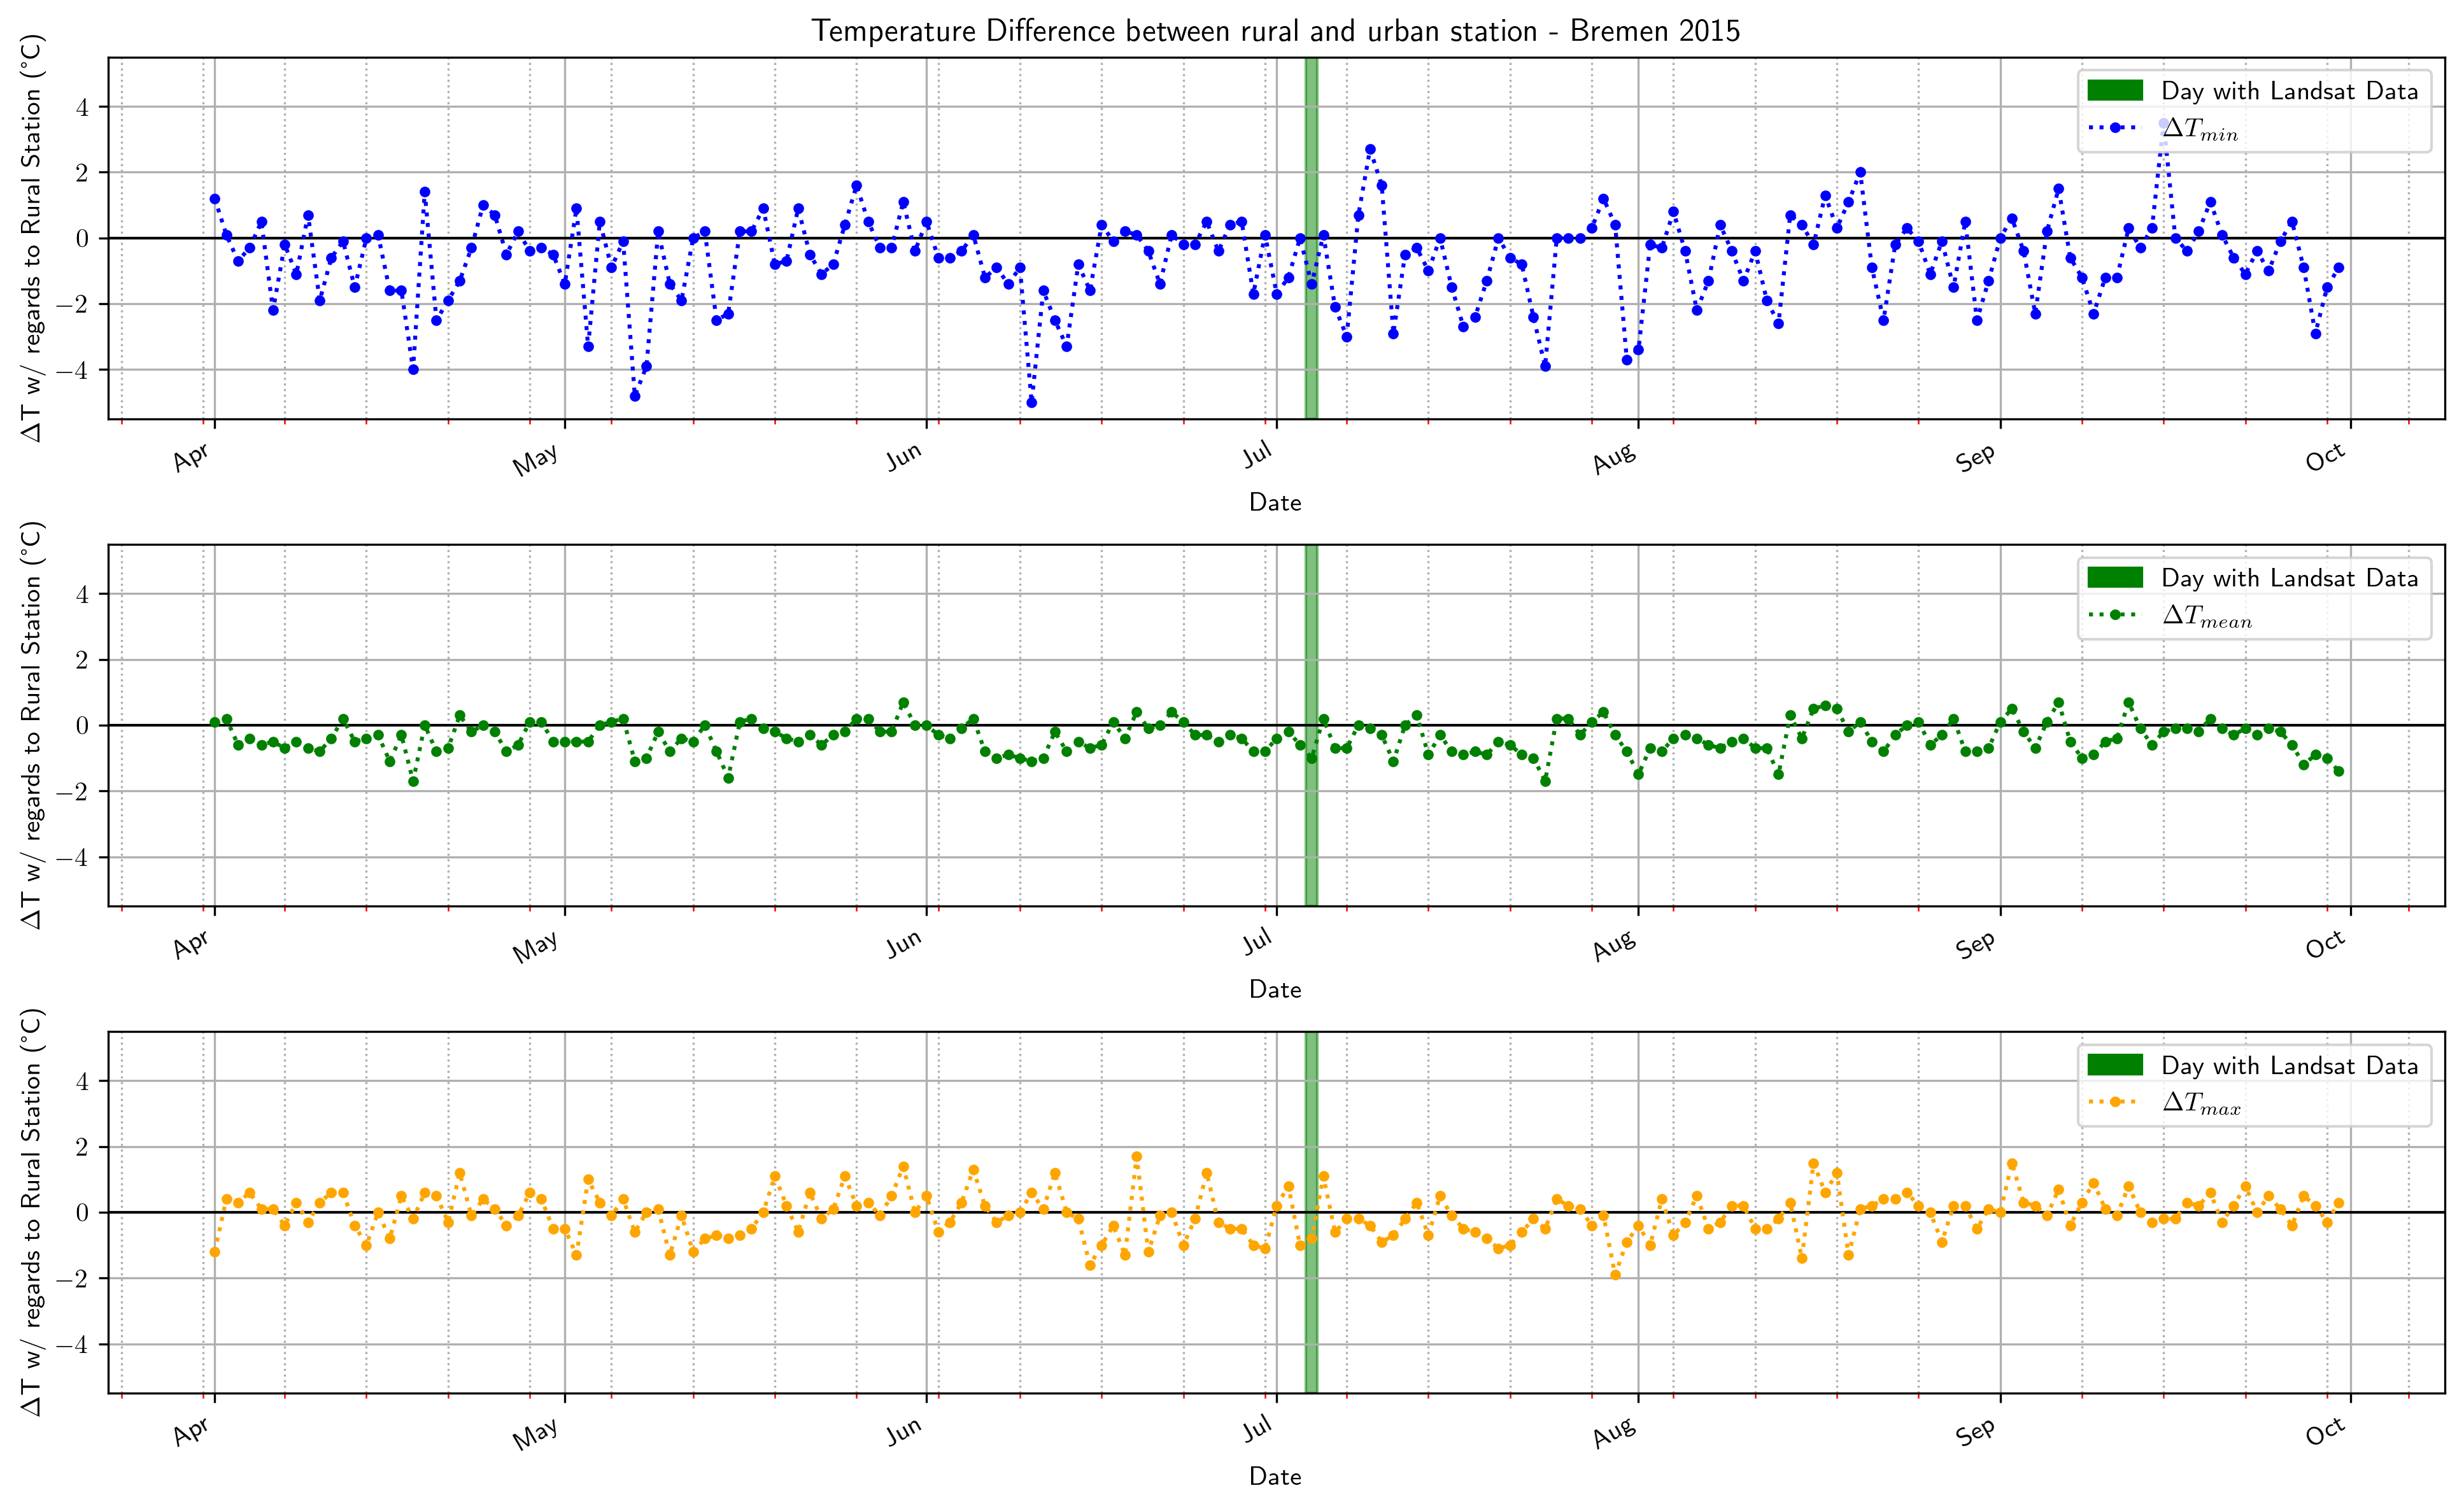
\includegraphics[width=\textwidth]{img/BremenDifferences2015.png}
        \subcaption{Absolute Differences between measurement stations [°C] and days with satellite coverage (green) in 2015}\label{fig:diff2015Bre}
       \end{subfigure}
       \begin{subfigure}[b]{\textwidth}
        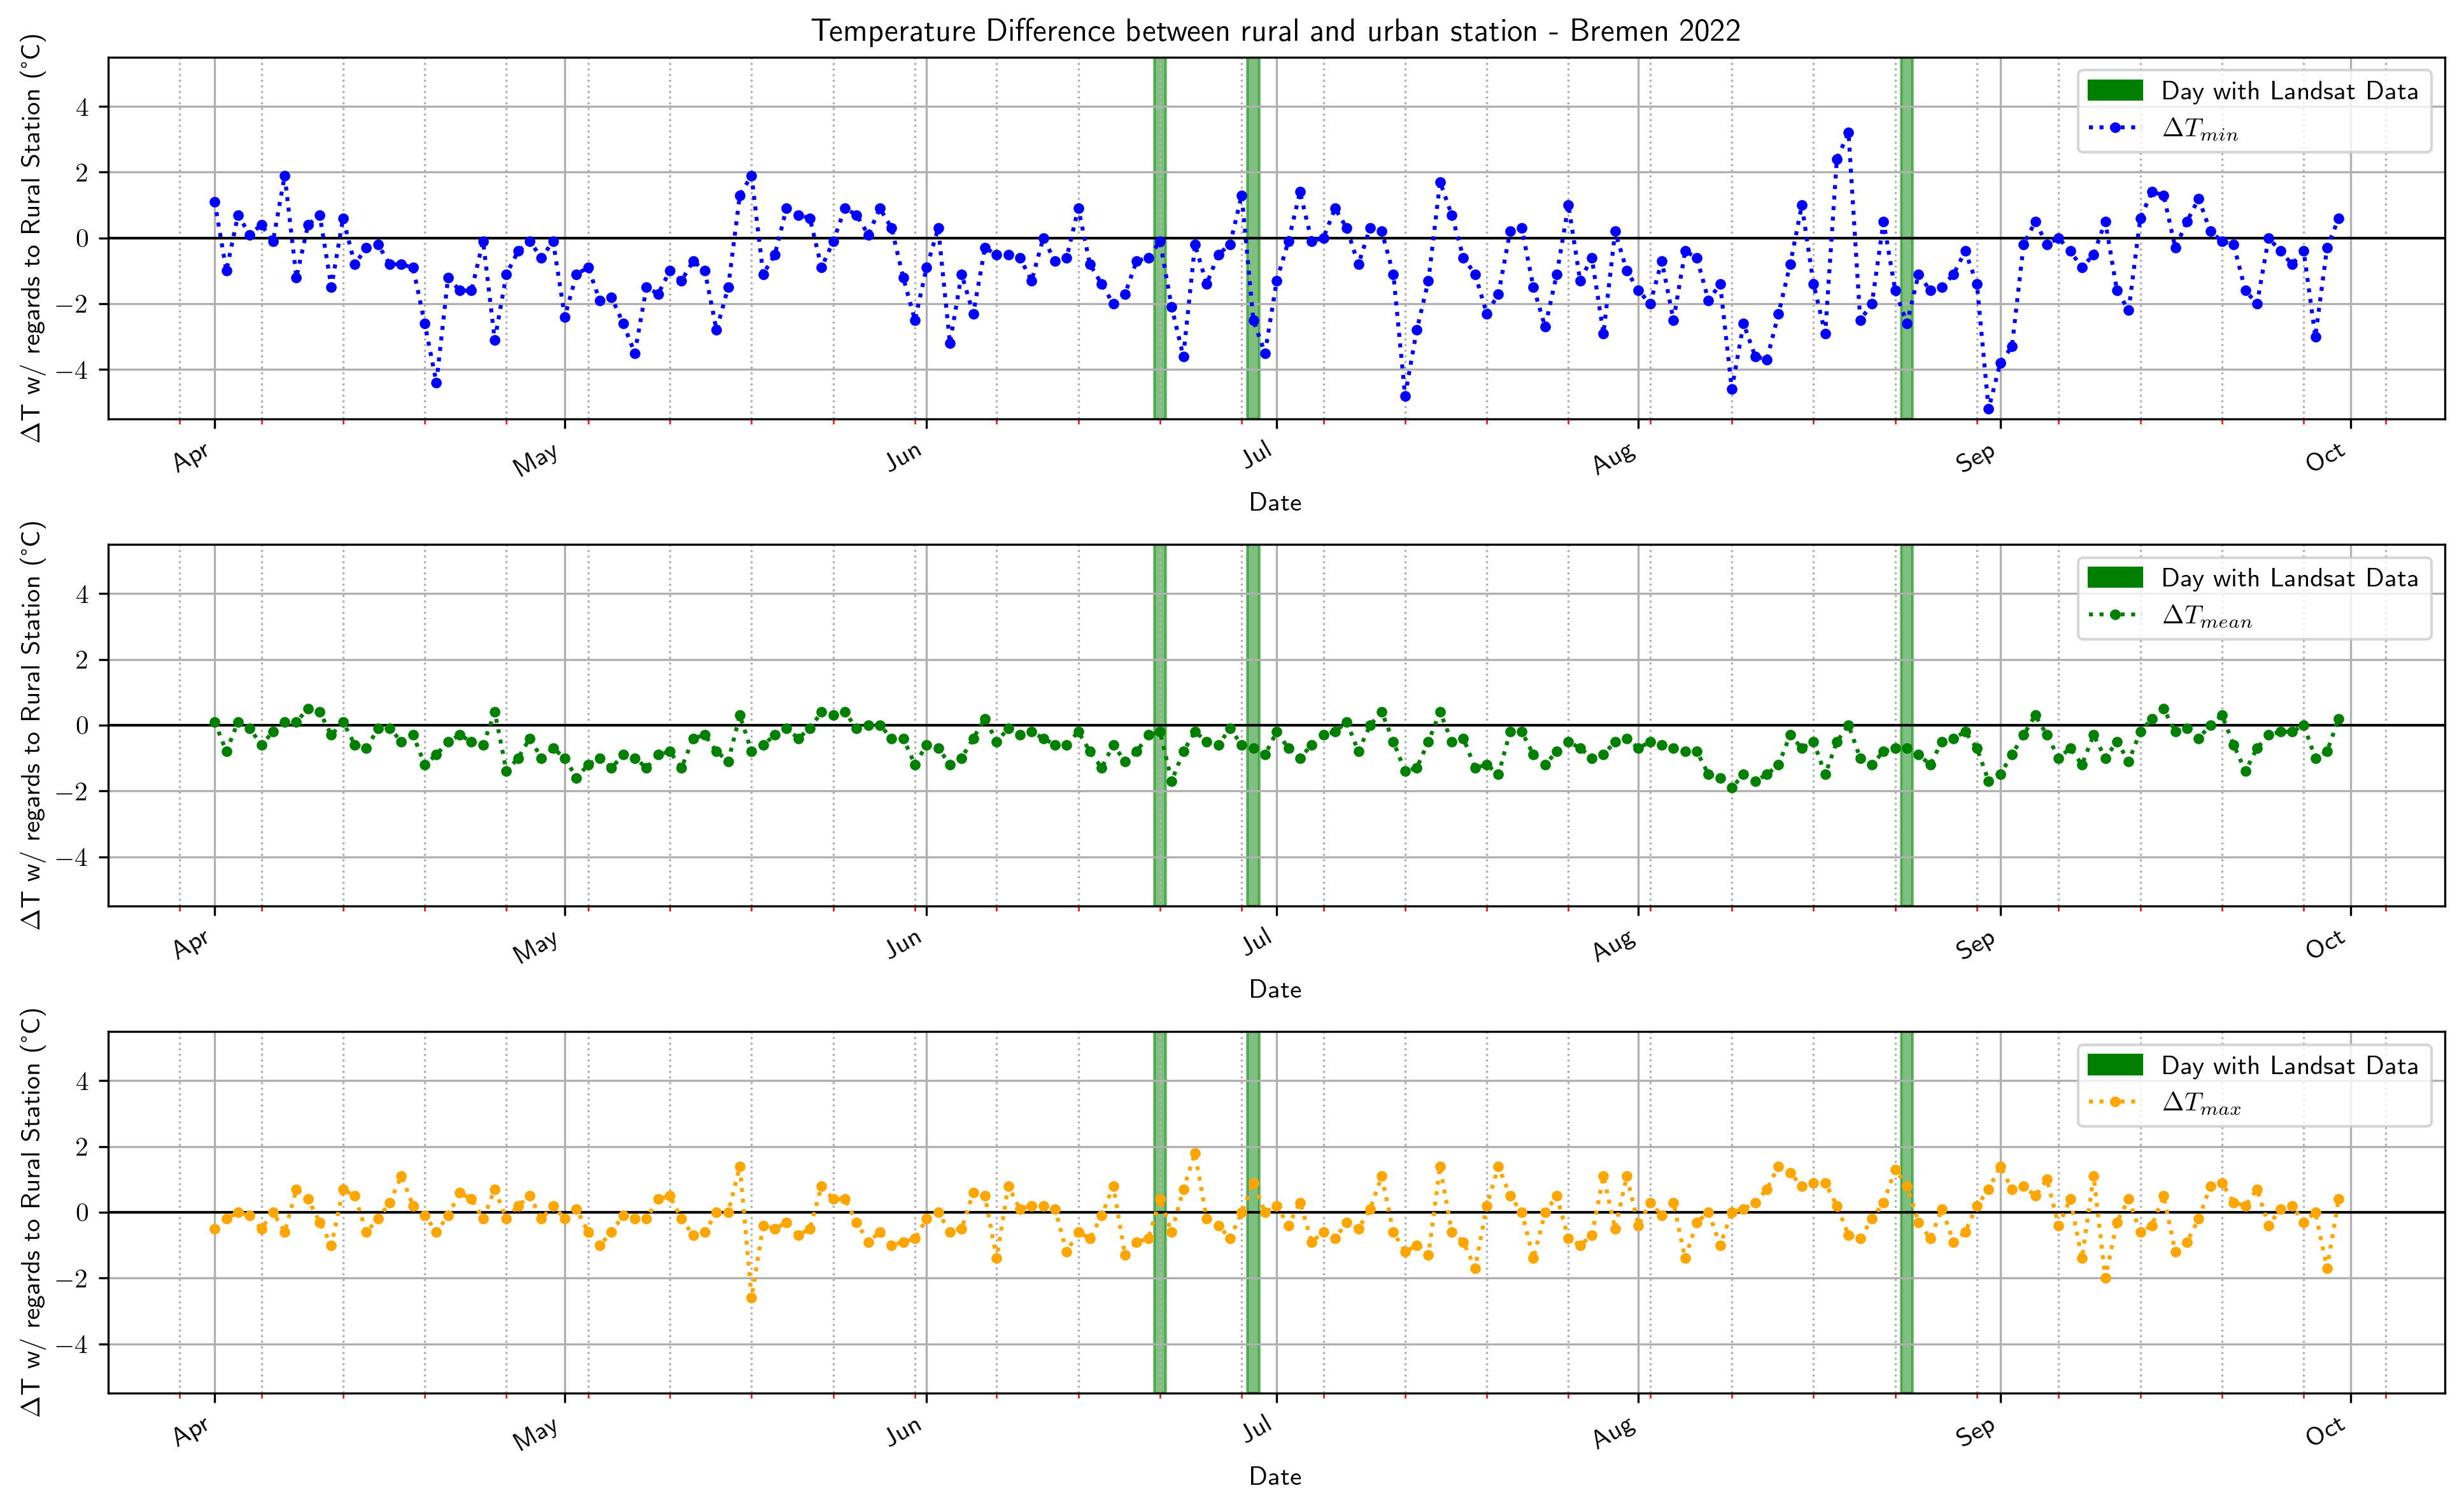
\includegraphics[width=\textwidth]{img/BremenDifferences2022.png}
        \subcaption{Absolute Differences between measurement stations [°C] and days with satellite coverage (green) in 2022}\label{fig:diff20222Bre}
       \end{subfigure}
         \caption{Differences of weather station measurements in urban and rural areas near Bremen}\label{fig:diffBre}
   \end{figure}
   %To test if the temperature in the weather stations was significantly offset a \gls{WilMannWhitTe} was performed on the datasets.
   %The test showed a significant offset for the minimum and mean temperature.



\begin{figure}[!p]
     \centering
       \begin{subfigure}[b]{\textwidth}
          \includesvg[width=\textwidth]{img/UHIs_Bremen_2019-06-29_s:3.svg}
         \subcaption{Map of the detected UHIs in June 2019}\label{fig:uhis2019}
       \end{subfigure}

       \begin{subfigure}[b]{\textwidth}
          \includesvg[width=\textwidth]{img/UHIs_Bremen_2022-06-21_s:3.svg}
         \subcaption{Map of the detected UHIs in June 2022}\label{fig:uhis2022}
       \end{subfigure}
         \caption{Overview of Bremen UHIs at different times \glspl{UHI}}\label{fig:AnalysisBre}
   \end{figure}
%

%
 % \subsubsection{Essen}
 % Essen is a city located in the centre of the Ruhr in Germany, with a population of 583000.  \\
%%
 % The weather station ``Essen-Brederney'' is located at the edge of the ``Brederney'' suburb to the north of the city located 6.8 km from the city centre (nearly double the distance compared to Bremen). 
 % The overall climate in Essen is a mixture between ``warm-summer-humid-continental'' (Dfb) and ``temperate-oceanic'' (Cfb) climate according to the Köppen-Geiger climate classification scheme.
 % The average and extrem values from the ``Essen-Brederney'' station are shown in \cref{tbl:essenweather}.
 % The reference station is the station ``Duisburg-Bearl'' located 30 km to the south west next to the river Rhine.\\
 % \begin{table}[ht]
 %   \centering
 %   \renewcommand{\arraystretch}{1.4}
 %   \caption{Essen weather data using~\autocite{DWD2024b} data\label{tab:essenweather}}
 %   \begin{tabular}{p{3.5cm}p{2.5cm}lp{2.5cm}}
 %     \toprule
 %     & \textbf{Extremly Cold} & \textbf{Average} & \textbf{Extremly Warm} \\
 %     & min & mean & max \\
 %     \midrule
 %     Annual average °C \newline (Jahr)     &   8.2 \newline(1956)     & 10.1   & 12.0 \newline (2022)      \\
 %     Abs. T °C \newline (Jahr)             & -24 \newline(Feb. 1940)  &        & 40   \newline (Aug. 1992) \\
 %     Summer days \newline($T_{\max}~\ge$  25 °C) & 5                  & 28.5   & 78 \\
 %     Hot days \newline($T_{\max}~\ge$  30 °C)    & 0                  & 4.9    & 17 \\
 %     \midrule
 %     & max & mean & min \\
 %     \midrule
 %     Frost days \newline($T_{\min}~<$  0 °C)     & 95   & 50     & 11 \\
 %     Ice days \newline($T_{\max}~<$  0 °C)       & 48   & 11.4   & 0  \\
 %     \bottomrule
 %   \end{tabular}
 % \end{table}
%%
%%
 % Essen is located on a stripe of overlapping Landsat paths and is covered completely by path 196 and 197, providing a much denser satellite data cover of that area.
 % In total there where 77 Images with no cloud cover over Essen between 2015--01--01 and 2023--12--31.
%
%   
\begin{landscape}
    \begin{table}[ht]
    \renewcommand{\arraystretch}{1.4}
    \centering
    \caption{Comparison of Air Temperature, \gls{LST} and \gls{UHI} size for Bremen\label{tab:statsBremen}}
    \begin{tabular}{l lll lll l lll c lll}
      \toprule
        &\multicolumn{7}{c}{\makecell{\textbf{Air Temperature}}} & \multicolumn{3}{c}{\makecell{\textbf{LST}}}\\
      \textbf{Date}&\multicolumn{3}{c}{\makecell{\textbf{Urban}}} &\multicolumn{3}{c}{\makecell{\textbf{Rural}}} & \textbf{$\Delta T$} &
      \multicolumn{3}{c}{\makecell{\textbf{Urban}}}& \multicolumn{3}{c}{\makecell{\textbf{Rural}}}\\

        & $T_{\min}$ & $T_{mean}$ & $T_{\max}$ & $T_{\min}$ & $T_{mean}$ & $T_{\max}$ & & 
       $T_{\min}$ & $T_{mean}$ (std) & $T_{\max}$ & Num. UHIs & $T_{\min}$ & $T_{mean} (std)$ & $T_{\max}$ \\
           \midrule
      2022--06--21 & 6.9 & 15.7 & 22.3 & 7.6 & 15.6 & 23.0 & -1.0 & 4.4 & 29.0 (4.4) & 56.7 & 39 & 4.7& 29.7 (4.4)& 56.7 \\
      2019--06--29 & 15.9 & 24.7 & 31.9 & 17.7 & 25.4 & 30.7 & -0.7 & 22.9 & 34.2 (3.5) & 61.4 & 120 & 22.92 & 35.2(3.77) & 61.4 \\
      .... TBC & & & & & & & & & &&&&&\\
      \bottomrule
    \end{tabular}
  \end{table}

  \begin{table}[ht]
    \renewcommand{\arraystretch}{1.4}
    \centering
    \caption{Comparison of Urban Heat Islands in Bremen over time \label{tab:statsBremen}}
    \begin{tabular}{l lll ll}
      \toprule
      \textbf{Date}& Number UHIs & min area & mean area & max area & min UHI mean T & max UHI \\
           \midrule
       2022--06--21 & 120 &  \\ 
      2019--06--29 & \\
      .... TBC & & & & & & & & & &&&&&\\
      \bottomrule
    \end{tabular}
  \end{table}


 % \begin{table}[ht]
 %   \centering
 %   \renewcommand{\arraystretch}{1.4}
 %   \caption{Comparison of Air Temperature, LST and Urban Heat Island size for Essen\label{tab:statsEssen}}
 %   \begin{tabular}{l lll lll l llll lll}
 %     \toprule
 %       &\multicolumn{7}{c}{\makecell{\textbf{Air Temperature}}} & \multicolumn{3}{c}{\makecell{\textbf{LST}}}\\
 %     \textbf{Date}&\multicolumn{3}{c}{\makecell{\textbf{Urban}}} &\multicolumn{3}{c}{\makecell{\textbf{Rural}}} & \textbf{$\Delta T$} &
 %     \multicolumn{3}{c}{\makecell{\textbf{Urban}}}& \multicolumn{3}{c}{\makecell{\textbf{Rural}}}\\

 %       & $T_{\min}$ & $T_{mean}$ & $T_{\max}$ & $T_{\min}$ & $T_{mean}$ & $T_{\max}$ & & 
 %      $T_{\min}$ & $T_{mean}$ & $T_{\max}$ & Num. UHI & $T_{\min}$ & $T_{mean}$ & $T_{\max}$ \\
 %          \midrule
 %     2015--07--04 & 18.3 & 26.3 & 36.0 & 19.7 & 27.3 & 36.8 & -1.0 & & & & & & & \\
 %     2021--06--18 & 15.9 & 24.7 & 31.9 & 17.7 & 25.4 & 30.7 & -0.7 & & & & & & & \\
 %     2021--06--02 & 8.3  & 18.1 & 25.7 & 10.6 & 18.3 & 24.4 & -0.2 & & & & & & & \\
 %     2022--06--21 & 6.3  & 15.6 & 23.4 & 6.4  & 15.8 & 23.0 & -0.2 & & & & & & & \\
 %     2022--08--24 & 15.8 & 24.2 & 32.0 & 18.4 & 24.9 & 31.2 & -0.7 & & & & & & & \\
 %     2022--06--29 & 10.7 & 20.8 & 29.0 & 13.2 & 21.5 & 28.1 & -0.7 & & & & & & & \\
 %     \bottomrule
 %   \end{tabular}
 % \end{table}
\end{landscape}
%\subsection{Analysis}
%\subsection{Conclusions}{sec:conclusion}

%    \newpage
%    \section{Simulation and Modeling of \texorpdfstring{\glsxtrlongpl{UHI}}{Urban Heat Islands}}\label{sec:modelling}
%    \subsection{Introduction}
%
%    \subsection{Analysis}
%    \subsection{Conclusions}
%\newpage
%\section{Discussion}\label{sec:discussion}
%    \subsection{Synthesis of Findings}
%    \subsection{Implications}
%
\newpage
\section{Conclusion}\label{sec:conclusion}
\subsection{Summary}
% Summary of the findings 
% contributions to research

\subsection{Limitations and Challenges}
% Why was something not possible
While the connection of ground based sensor stations with remote imagery works well, a direct reliable conversion from land surface temperatures to air temperature, since there is a temporal and seasonally different energy transport between surfaces and surrounding air. 
Another limiting factor was the availability of suitable cloud free satellite footage of the area of study.
While with the introduction of Landsat 9, the amount of footage doubled, in regions 

\subsubsection{Data}
\subsubsection{Software}

% 
\subsection{Future Work}
The classification part should be improved by using a widely available product that has a suitable resolution. 
During development the 300 m reference product \cref{sec:references} was used but was not considered precise enough for these measurements.

\newpage
\section{Appendix}
\subsection{Additional Figures}
%TODO 
\subsection{Content of the Data Storage device}
All data and the software used to create the figures and images for this document are available on the storage device.
The software is also available online in the linked GitHub repository.
The software version last used for this document is tagged with the name: \texttt{master-submission}
The following artefacts can be found in these locations:
\subsubsection{Data}
The data is stored in multiple subfolders. 
The \texttt{Data} folder contains the different cities as subfolders, within each of these folders, there is a \texttt{dataset} folder, containing a \texttt{xarray} dataset named \texttt{dataXarrayCITY_NAME.nc} of the used area of interest, including all bands and the classifiction at all times analysed during this project. 
The \texttt{dataXarrayCITY_NAME_feat.nc} contains the extracted feature bands from the gabor feature extraction.
The \texttt{ML_Model} folder contains a ``pickeled'' K-Means model, a file containing a numpy array with cluster centres for the label assignment and the random forest model. %TODO CHECK for rf
\subsubsection{Code}
The folder app contains the python code used for generating the data, the documentation of the code is located within the doc folder.
%
%
\newpage
\printbibliography%
\newpage
\section*{Eigenständigkeitserklärung}

\includepdf[pages=-]{res/eigenstaendigkeitserklaerung.pdf}
  % TODO insert Eigenständigkeitserklärung
\end{document}

%The surface classes where correlated with the %TODO check 
%Kataster data from Bremen as well as with OSM data. % todo do 
%
%Ziel Projekt teil: 
%- detection and error margins in UHI detection using remote sensing data 
%- data pipeline to create maps of UHI in areas 
%- surface classification based on remote sensing data correlated with 2nd and 3rd sources (kataster/ OSM) 
%- UHI "cores" identification 
%
%Master Fragestellungen: 
%- Correlation zw. UHI} und Pollutants? 
%https://pubs.acs.org/doi/epdf/10.1021/cr5006815 
%- Real time UHI size/occurrence prediction based on ground temperature stations (Bremen Airport) and pollutant levels? 
%- UHI classification in different environments, causes and effects, mitigation stategies? (e.g. Classification of Surface types, vegetation etc. within different climate zones (Phoenix, Bremen, Karlruhe, Essen, Something meditareiean, Afrika (coastal, arid, etc) /paper with adis abbeba)
%
%\subsection{}

%Of the different bands available from the used satellite data (Landsat7 and Landsat8), 
%the visible and near infrared bands where used for clustering. 
%The clustering was done using the simple k-means algorithm. 
%Different configuration where used %todo add pictures? 
%These where compared and referenced with ground truth data %todo add error and limitations refgerenec here 


